\documentclass{notes}
\usepackage[french]{babel}
\usepackage{pdfpages}
\usepackage{minitoc}

\usepackage{eurosym}

\usepackage{subfig}

% for bullet point in french
\AtBeginDocument{\def\labelitemi{$\bullet$}}

\usepackage[
type={CC},
modifier={by-nc-sa},
version={3.0},
]{doclicense}

\newcommand{\py}{\lstinline{Python} }


\begin{document}





\begin{titlepage}
\begin{center}
\fbox{
\begin{minipage}{16cm}
\begin{center}
 \vspace{12pt}
\scalebox{0.88}{{\Huge \textbf{	Introduction à l'informatique}
}}

%\vspace{12pt}
%
%\scalebox{1}{{\Huge \textbf{Polycopi\'e}
%}}

\vspace{18pt}
{\Large Collège Sismondi }
\vspace{12pt}
\end{center}

\end{minipage}
}\\
\vspace{30pt}
{\huge Mathieu Schiess}\\
\vspace{80pt}
\begin{center}


	  
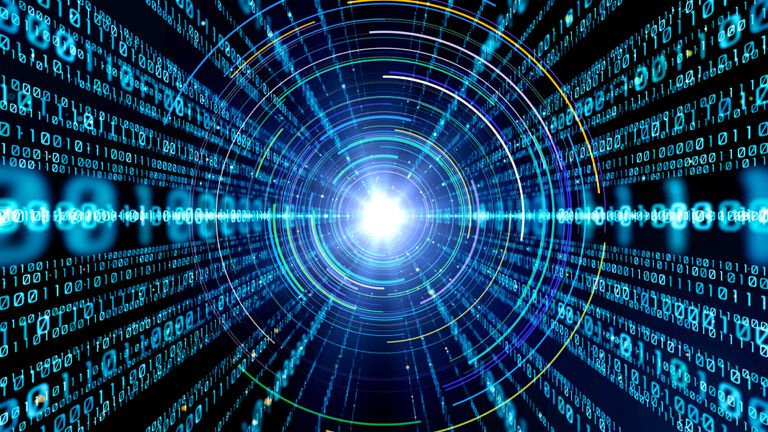
\includegraphics[width=\textwidth]{Images/computerlight.jpg}
\end{center}
%\hspace{8.5cm} {\scriptsize Sources: \url{http://www.josleys.com}}


\end{center}
%%%%%%%%%%%%%%%%%%%%%%%%%%%%%%%%%%%%%%
%%%%%%%%%%%%%%%%%%%%%%%%%%%%%%%%%%%%%%
\end{titlepage}





\clearpage
\doclicenseThis
\clearpage
\renewcommand{\thepage}{\roman{page}}
\setcounter{page}{1}

\dominitoc
\tableofcontents
%\listoffigures
%\listofmyequations

\clearpage
\renewcommand{\thepage}{\arabic{page}}
\setcounter{page}{1}


%\mainsection{1}{Lecture Title}{dd/mm/yyyy}

\section{Title 1}

\subsection{Title 1.1}
	You can use the custom putfigure command to add figures to the document. the command takes 6 arguments - how much horizontal size to create a bounding box, width, height, path to image, caption, label.
	
\verb!\putfigure{1.0}{0.7}{0.3}{Images/rl1}{Many Faces of RL}{fig1_1}! \\

\putfigure{1.0}{0.7}{0.3}{Images/rl1}{Many Faces of RL}{fig1_1}

\subsection{Title 1.2}

\section{Title 2}
	Adding multiple images using putfigure with minipage \\
\verb!\begin{minipage}{\textwidth}! \\
\verb!    \centering! \\
\verb!        \putfigure{0.49}{1.0}{0.2}{Images/rl2}{A generic RL schematic diagram}{fig1_2}! \\
\verb!        \putfigure{0.49}{1.0}{0.2}{Images/rl3}{An RL agent with environment loop}{fig1_3}! \\
\verb!\end{minipage}! \\

\begin{minipage}{\textwidth}
	\centering
		\putfigure{0.49}{1.0}{0.2}{Images/rl2}{A generic RL schematic diagram}{fig1_2}
		\putfigure{0.49}{1.0}{0.2}{Images/rl3}{An RL agent with environment loop}{fig1_3}
\end{minipage}

	You can use the myequations command to add any equation to the list of equations in contents. Just pass the name for that equation with the command \\


\verb!\begin{align}! \\
\verb!    \S_t = \f(\H_t)! \\
\verb!\end{align}! \\
\verb!\myequations{Generic state RL system}! \\

\begin{align}
	\S_t = \f(\H_t)	
\end{align}
\myequations{Generic state RL system}

% Thème Informations et données
\mainsection{\the\numexpr \thechapter + 1 \relax}{Introduction}{02/09/2021}

%Théorie :
%Comprendre la différence entre donnée et information. Introduire la notion d’encodage de l’information.
%Pratique :
%Savoir encoder en binaire un entier positif. Savoir écrire en base 10 un nombre écrit en binaire. Savoir encoder un caractère en ASCII étendu à l’aide d’une table. Être capable de décoder un texte bref écrit en ASCII étendu à l’aide d’une table.

\section{C'est quoi l'informatique?}
\begin{mydefinition}
	L'\textbf{informatique} est la science du traitement automatique de l’information.
\end{mydefinition}
Le traitement automatique de l’information est accompli par un système (dans la pratique une machine) appelé \textbf{ordinateur} qui est capable de stocker et traiter (modifier, lire et écrire) de l'information. On peut aussi dire que le but de l'informatique est d'étudier comment les ordinateurs peuvent résoudre des problèmes.

Schématiquement, un ordinateur est une machine qui transforme des données en entrée, qui sont les données bruts du problème, afin de produire le résultat attendu (données de sortie).
\begin{center}
	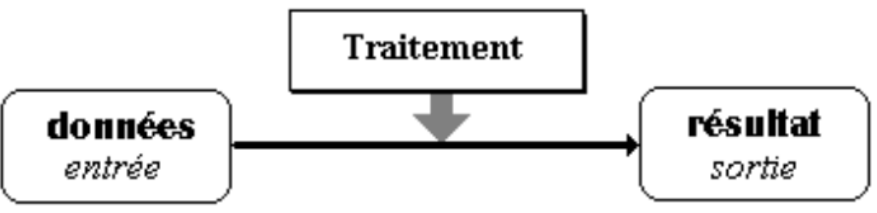
\includegraphics[trim=0 0 0 20,width=0.5\textwidth]{Images/shema_science_info}
\end{center}
Dans ce cours, on considérera toujours qu'un ordinateur est une machine électronique. A ce stade, si l'on souhaite automatiser le traitement d'informations, il y a plusieurs problèmes à résoudre:
\begin{enumerate}
	\item Comment un ordinateur, qui sait seulement lire des signaux électriques, est-il capable de lire et stocker de l'information? Ce sujet s'appelle la \textbf{représentation numérique de l'information}.
	\item Comment décrire et trouver un processus automatique qui permette de résoudre notre problème?
	Ce processus s'appelle un \textbf{algorithme} et l'étude de ce sujet s'appelle l'\textbf{algorithmique}.
	\item Comment \textit{indiquer} à un ordinateur la manière dont il doit appliquer un algorithme? Cette question sera abordée lorsque nous étudierons les \textbf{langages de programmation}.
\end{enumerate}

\begin{myexamples}

	\itemb{Jeu vidéo}

	\begin{itemize}
		\item Entrée: Boutons et touches pressés sur une manette de jeu
		\item sortie: Déplacement du personnage.
	\end{itemize}

	\begin{center}
		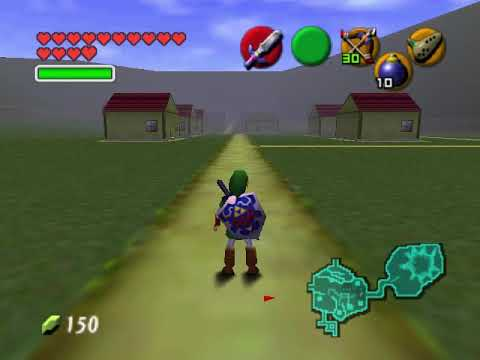
\includegraphics[trim=0 0 0 0,width=0.25\textwidth]{Images/intro/zelda2.jpg}
	\end{center}
	
	\itemb{chirurgie assistée par ordinateur}
	\begin{itemize}
		\item Entrée: Mouvements d'un chirurgien (avec tremblements).
		\item sortie: Mouvements de bras de robots  (sans tremblement).
	\end{itemize}
	\begin{center}
		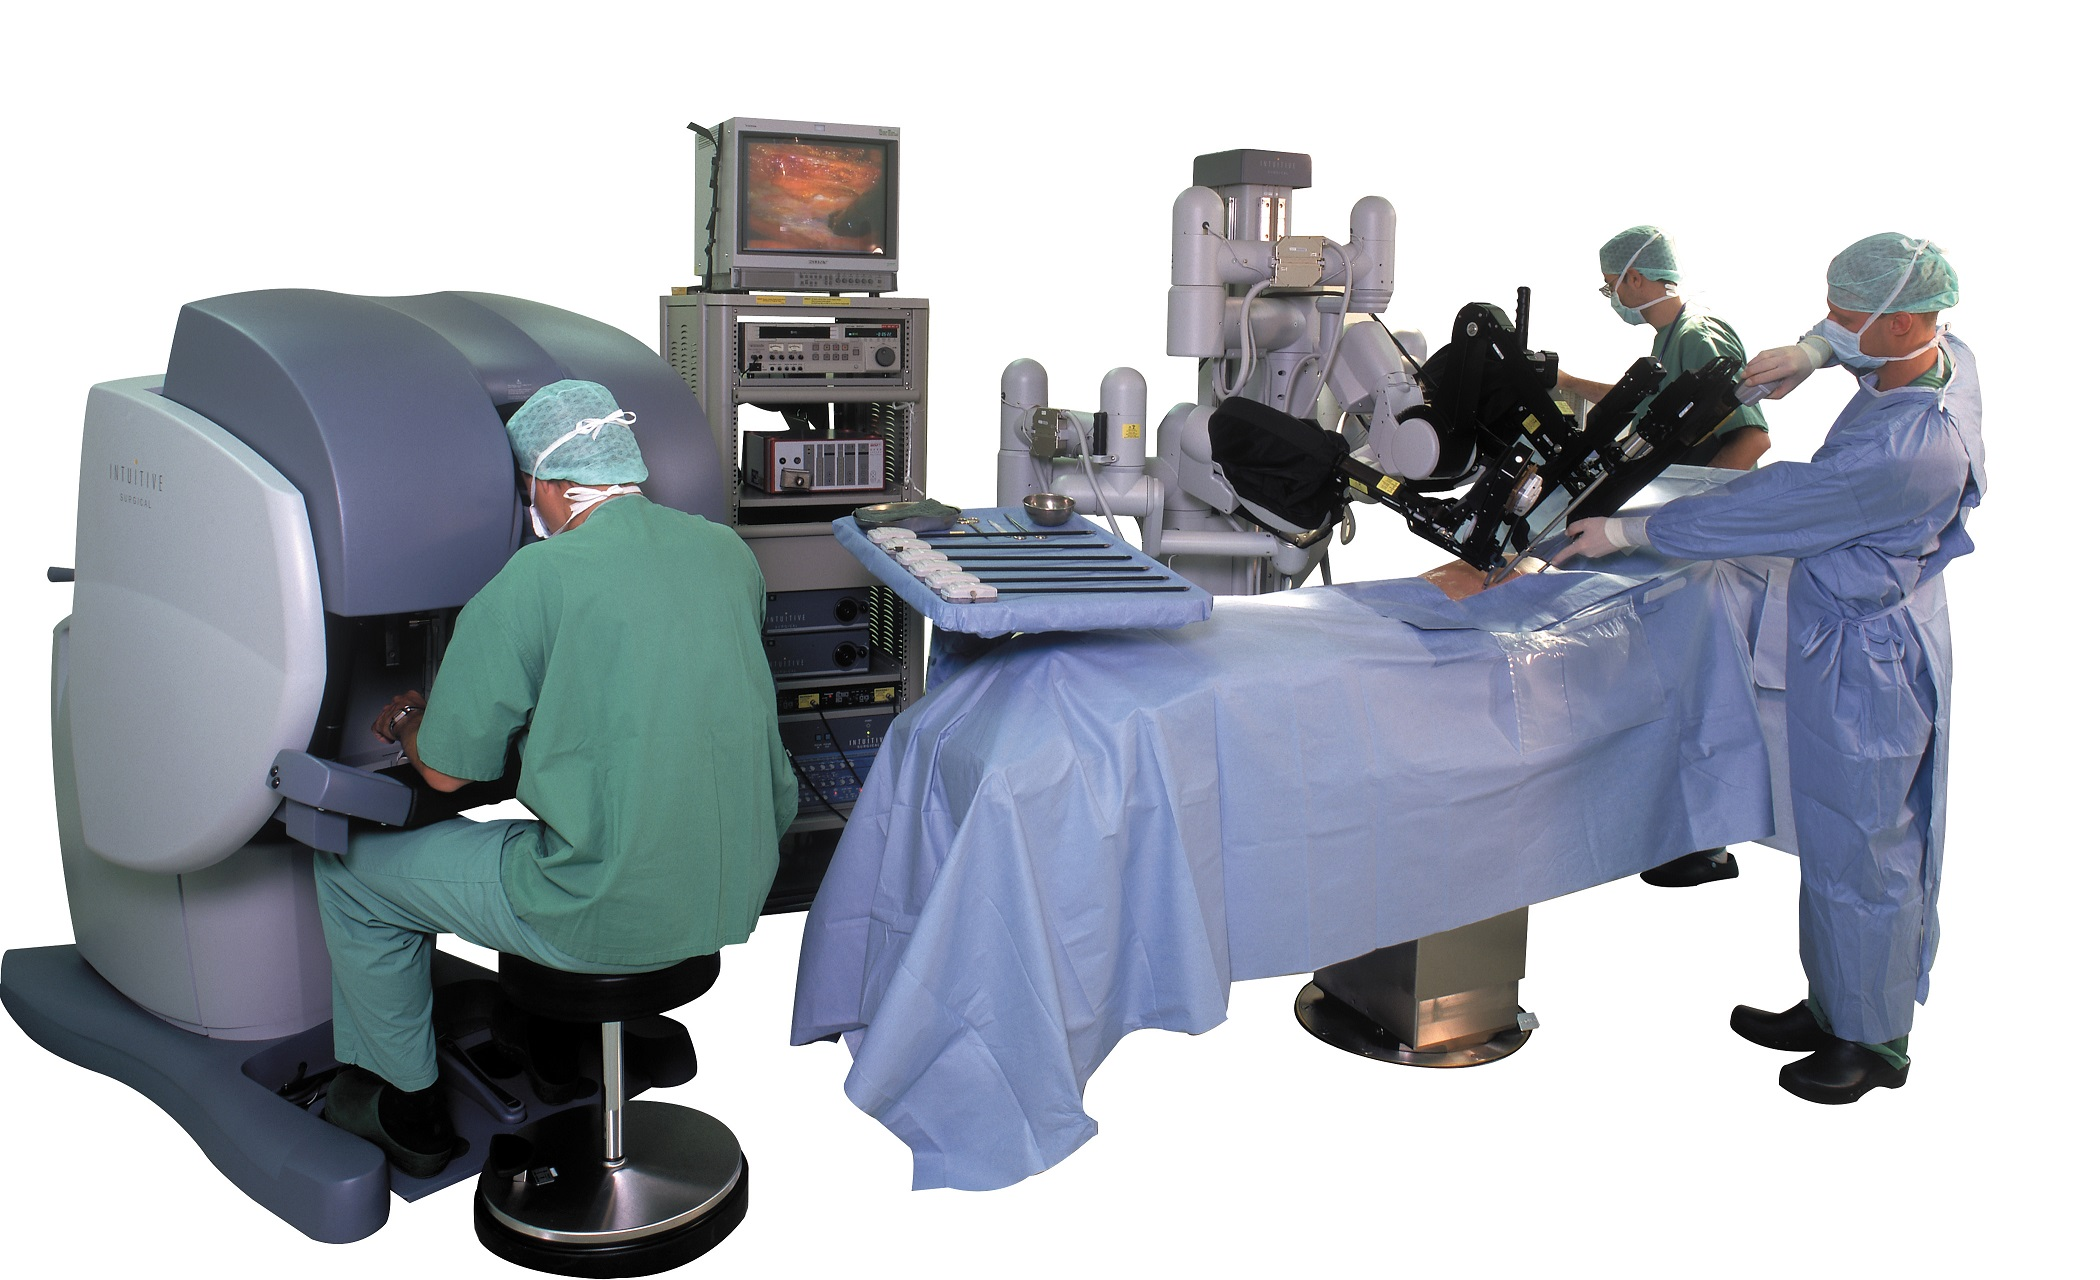
\includegraphics[trim=0 0 0 20,width=0.4\textwidth]{Images/intro/da-vinci-robot-chirurgien.jpg}
	\end{center}

	\itemb{Détection de cancer}
		\begin{itemize}
			\item Entrée: images médicales (radios, IRM, ...)
			\item sortie: Détermine si il y a une tumeur et dans ce cas où elle se situe
		\end{itemize}	
	\begin{center}
		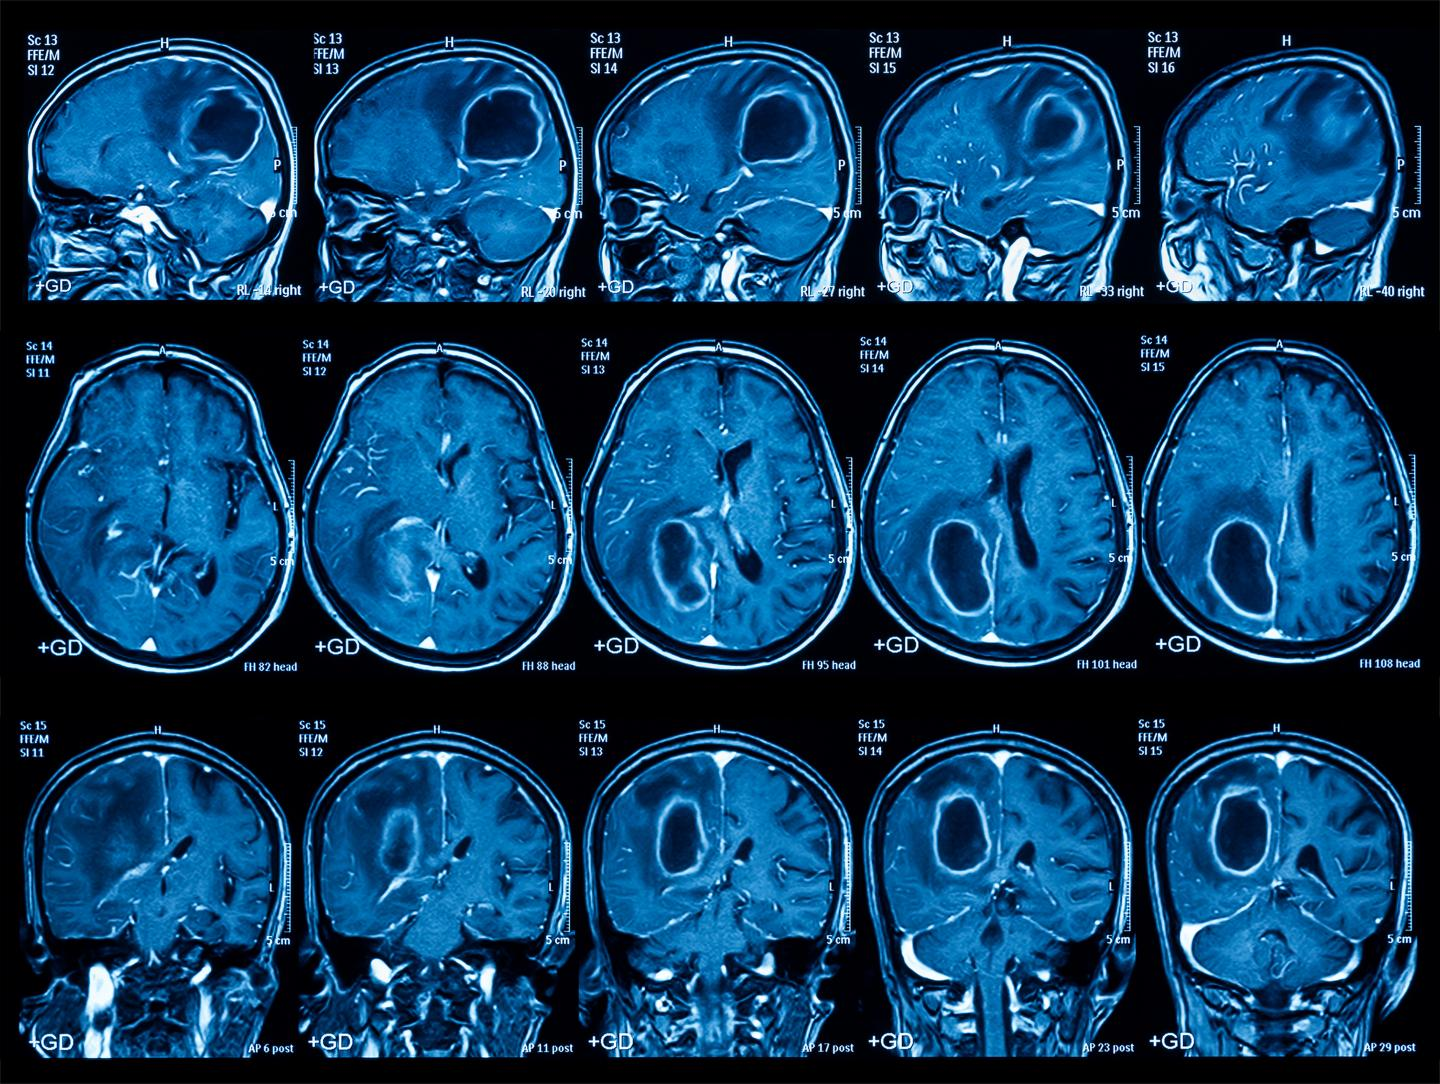
\includegraphics[trim=0 0 0 0,width=0.25\textwidth]{Images/intro/MRI_SCAN.jpg}
	\end{center}
\newpage
	\itemb{Médias sociaux, par exemple youtube}
	\begin{itemize}
		\item Entrée: les vidéos que j'ai regardé + les données de visionnage.
		\item sortie: Un liste de vidéos que je devrais apprécier.
	\end{itemize}
	\begin{center}
		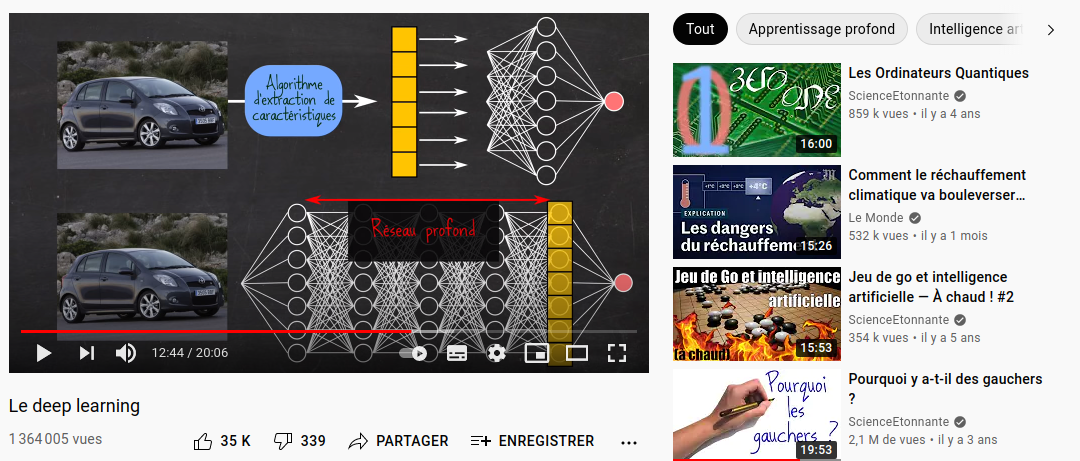
\includegraphics[trim=0 0 0 0,width=0.4\textwidth]{Images/intro/ex_youtube.png}
	\end{center}

\end{myexamples}


\begin{eclairage}
	Dans le chapitre précédent nous avons parlé tantôt d'information tantôt de données. Ce sont deux concepts assez proche 
	\begin{itemize}
		\item En informatique, l’\textbf{information} est un élément de connaissance (texte, image, son, etc.) susceptible d’être numérisé, stocké et/ou transmis à l’aide d’un support et d’un mode de codification normalisé
		\item Une \textbf{donnée} est la représentation d’une information sous une forme
		conventionnelle (codée) destinée à faciliter son traitement.
	\end{itemize}
	Sans rentrer dans les détails, une information est un concept abstrait qui s'apparente plutôt à une idée, tandis que la donnée est une représentation. Par exemple l'information "arbre" peut être représentée, par exemple, avec un pictogramme ou avec un mot écrit avec des lettres:
	\begin{center}
		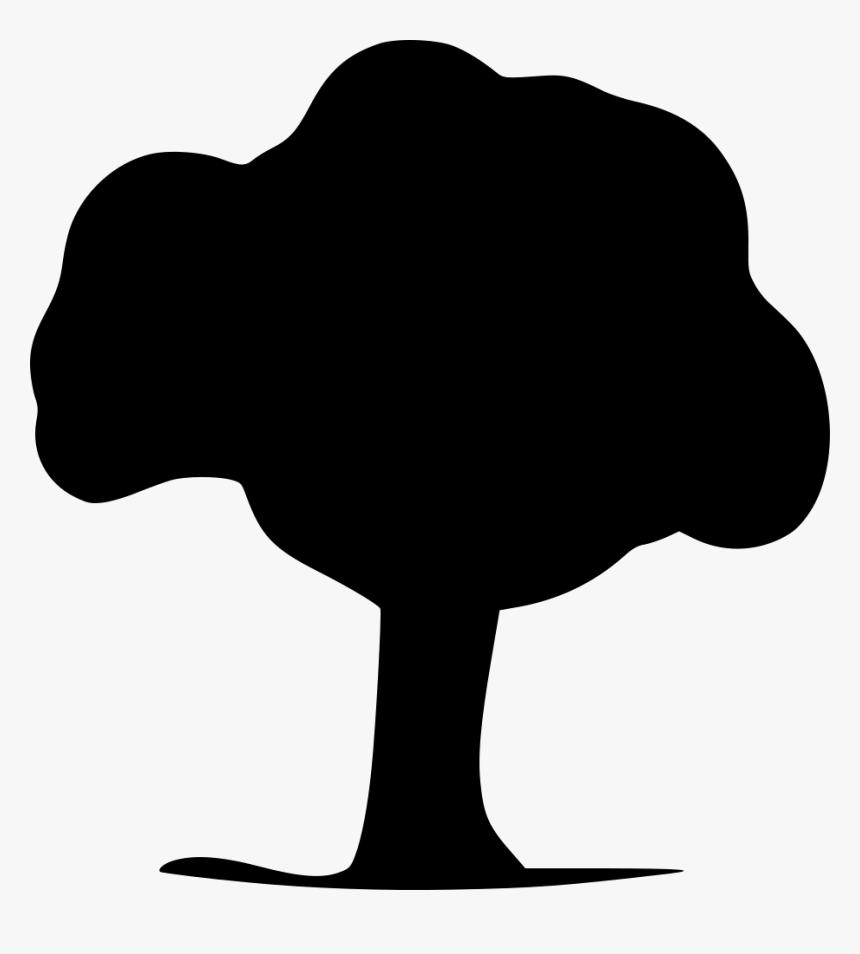
\includegraphics[trim=0 0 0 20,width=0.2\textwidth]{Images/intro/arbre.png} 
		\hspace{2cm}
		\fbox{\Huge ARBRE }
	\end{center}
\end{eclairage}	

\section{Représentation de l'information}
\label{codageNombre} 
A tout moment, tout fil de l’ordinateur se trouve à un voltage haut (1) ou bas (0) (la valeur exacte du voltage n’a pas d’importance).
\begin{figure}[!h]
	\centering
	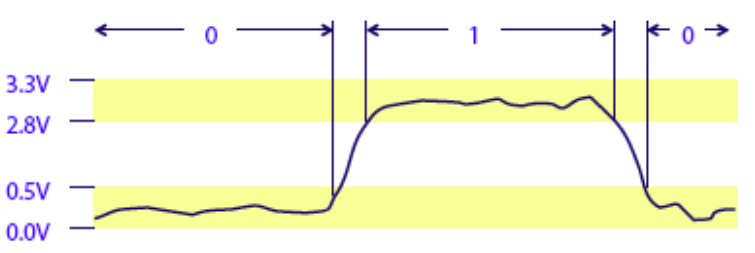
\includegraphics[trim=0 0 0 20,width=0.6\textwidth]{Images/intro/signaux.png} 
	\caption{Signal électrique mesuré dans un ordinateur}
\end{figure}
	
Donc tous les types d’informations possibles devront être représentées à partir d’une alternative entre deux états : courant ou pas courant ; allumé ou éteint ; vrai ou faux ; 1 ou 0. Cette quantité minimal d'information, qui ne prend que deux états 0 ou 1, est appelée \textbf{bit}.

\begin{mydefinition}
	Le terme {\bf bit} (b minuscule dans les notations) signifie {\it binary digit }, c'est-à-dire 0 ou 1 en numérotation binaire. Il s'agit de la plus petite unité d'information manipulable par une machine numérique. 
	\vspace{0.2cm}
	
	L'{\bf octet} (en anglais {\bf byte} ou B majuscule dans les notations) est une unité d'information composée de 8 bits. Il permet par exemple de stocker un caractère comme une lettre ou un chiffre.
\end{mydefinition}


\begin{question}
	Comment représenter n'importe quel type d'information, qui est susceptible d'être traitée (images, sons, textes, vidéos, ...) par un ordinateur, à l'aide seulement d'une suite de 0 et de 1? Autrement dit, comment représenter l'information avec un alphabet de deux symboles?
\end{question}


\section{Représentation des nombres entiers}
\subsection{Rappel : la représentation décimal des nombres}
Depuis le moyen âge, en occident, on représente les nombres entiers naturels en utilisant le \textit{système  décimale à position}. Pour ce faire, on dispose de dix symboles (comme nos dix doigts)
\begin{center}
	0, 1, 2 ,3 ,4 ,5 ,6, 7, 8 et 9.
\end{center}
Dans le \textit{système  décimale à position}, la position de chaque chiffre représente combien il y a de paquet de  10 de paquets de rang inférieur. Par exemple, un dizaine représente dix paquets d'unité, une centaine représente dix paquets de dizaines, etc... 
\begin{center}
	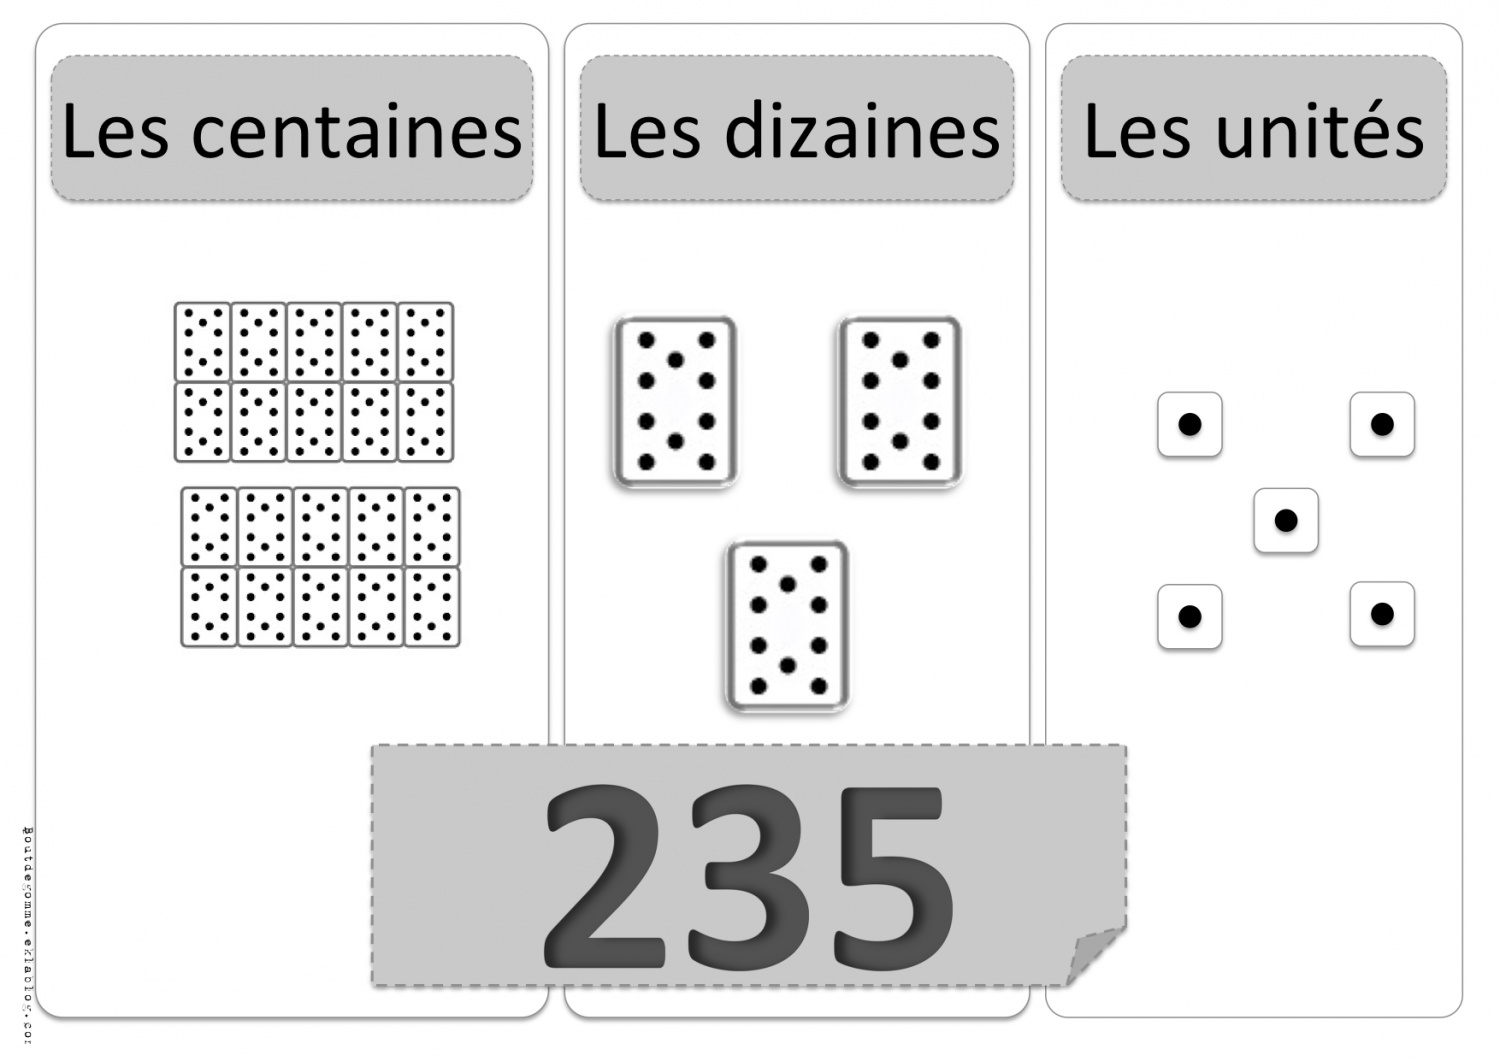
\includegraphics[trim=0 0 0 20,width=0.7\textwidth]{Images/intro/systeme_decimal.jpg}
\end{center}
Par exemple, l'écriture 235 indique qu'il y a 2 paquet de cent (cent représente dix paquets de dix), 3 paquets de dix et 5 paquets de un. Autrement dit on peut écrire
\begin{eqnarray*}
	235 &=&2 \cdot 100 + 3\cdot 10 +5 \cdot 1\\
	&=& 2 \cdot 10^2 + 3\cdot 10^1 +5 \cdot 10^0.
\end{eqnarray*}

\begin{eclairage}
Le choix de faire des paquets de dix est peut-être dû au fait que l’on a dix doigts,
mais on aurait pu tout aussi bien décider de faire des paquets de deux, de cinq, de
douze, de vingt, de soixante...
\end{eclairage}
\newpage

\subsection{Représentation binaire des nombres}
\act On considère les cartes suivantes 
\begin{center}
	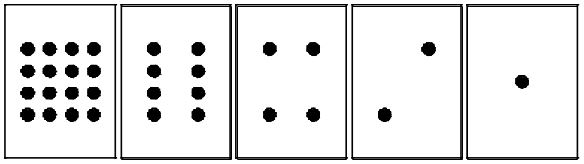
\includegraphics[trim=0 10 0 10,width=0.6\textwidth]{Images/intro/carte.jpg}
\end{center}
Chaque carte peut être dans deux états : 
\begin{itemize}
	\itemb{face visible} : les points sont visibles, c'est l'état 1.
	\itemb{face cachée} : la carte est retournée, c'est l'état 0.
\end{itemize}
\textbf{Questions}
\begin{enumerate}
	\item Quelles cartes faut-il retourner pour obtenir les nombres  3, 12 et 19.
	\item Existe-il plusieurs moyens de représenter un nombre avec ces cartes(par exemple pour les nombres 3, 12 et 19) ?
	\item Quels sont les plus petit et  grand nombres représentables avec ces cartes.
	\item Quel est le lien entre deux cartes successives?
	\item Utiliser les cartes pour représenter avec des bits (des 0 et des 1) les nombres 3, 12 et 19.
\end{enumerate}
\eexo \eexo
Pour représenter des nombres naturels en binaire, on s'inspire du \textit{système  décimale à position} mais avec seulement 2 symboles :	0 et 1. Un nombre entier est décomposé comme une somme de puissance de 2. 

Par exemple, $1011_{(2)}=1 \cdot 2^3 + 0 \cdot 2^2 +1 \cdot 2^1 + 1\cdot 2^0=11_{(10)}$ 

\begin{important}
	Dans ce cours, quand une suite de chiffres exprime un nombre dans une base différente de dix, on indique la
	base en index, par exemple : $1101_{(2)}$ (en base deux). Enfin, on rassemble parfois les bits par groupe de quatre ou de huit dans les mots très longs pour qu’ils soient plus faciles à lire : $1111111101$ est écrit $11 \,1111\, 1101_{(2)}$. Comme en base dix, ces groupes sont formés de droite à gauche.
\end{important}	

\subsubsection{Conversion binaire décimale}

Une autre façon d'obtenir le nombre en base 10, connaissant son écriture en base 2, est d'établir la valeur de chaque chiffre du nombre: celui le plus à droite représente 1, le deuxième représente 2, le troisième représente $2^2=4$, le quatrième représente $2^3=8$...  Par exemple si nous voulons connaître la valeur décimale du nombre 10 110, nous établissons d'abord une grille avec les différentes puissances de 2:

\begin{center}
	\begin{tikzpicture}
		\draw (-1,1) rectangle (0,0) rectangle (1,1) rectangle (2,0) rectangle (3,1) rectangle (4,0) rectangle (5,1) rectangle (6,0);
		\draw (5.5,0.5) node {$1$};
		\draw (4.5,0.5) node {$2$};
		\draw (3.5,0.5) node {$4$};
		\draw (2.5,0.5) node {$8$};
		\draw (1.5,0.5) node {$16$};
		\draw (0.5,0.5) node {$32$};
		\draw (-.5,0.5) node {$64$};
		
	\end{tikzpicture}
\end{center}

Ensuite, nous plaçons le nombre en binaire sous cette grille en mettant bien le chiffre des unités sous le carré le plus à droite et nous barrons les cases dont le chiffre associé est 0:

\begin{center}
	\begin{tikzpicture}
		\draw (-1,1) rectangle (0,0) rectangle (1,1) rectangle (2,0) rectangle (3,1) rectangle (4,0) rectangle (5,1) rectangle (6,0);
		\draw (5.5,0.5) node {$1$};
		\draw (4.5,0.5) node {$2$};
		\draw (3.5,0.5) node {$4$};
		\draw (2.5,0.5) node {$8$};
		\draw (1.5,0.5) node {$16$};
		\draw (0.5,0.5) node {$32$};
		\draw (-.5,0.5) node {$64$};
		
		\draw (5.5,-0.5) node {$0$};
		\draw (4.5,-0.5) node {$1$};
		\draw (3.5,-0.5) node {$1$};
		\draw (2.5,-0.5) node {$0$};
		\draw (1.5,-0.5) node {$1$};
		\draw (0.5,-0.5) node {$ $};
		\draw (-.5,-0.5) node {$ $};
		
		\draw (-1,0) -- (0,1)
		(0,0) -- (1,1)
		(2,0) -- (3,1)
		(5,0) -- (6,1);
		
	\end{tikzpicture}
\end{center}

Il ne reste plus qu'à additionner les nombres qui restent: $16 + 4 + 2=22$


\begin{myexamples}
	\item En décimal le nombre binaire $1100_{2}$ s'écrit
		  \vspace{1.5cm}
    \item En décimal le nombre binaire $10111_{2}$ s'écrit
    \vspace{1.5cm}
\end{myexamples}

\subsubsection{Conversion décimale binaire}

Pour trouver l'écriture binaire d'un nombre écrit en base 10, il existe principalement deux méthodes. 


\; 

La première méthode consiste à décomposer le nombre en somme de puissance de 2 et à utiliser la grille précédente. 

Plus concrètement, si nous voulons écrite 99 en binaire. La plus grande puissance de 2 que nous pouvons prendre dans 99 est 64 (128, la suivante, est trop grande). Il reste ensuite: 99-64=35. Dans 35 on peut mettre 32, et il restera 35-33=3. Dans 3 on ne peut ni mettre 16, ni mettre 8, ni mettre 4. On peut mettre 2. Il reste 1. Dans 1 on peut mettre 1. 

Cela signifie que 99=64+32+2+1. Sur notre grille cela donne:

\begin{center}
	\begin{tikzpicture}
		\draw (-1,1) rectangle (0,0) rectangle (1,1) rectangle (2,0) rectangle (3,1) rectangle (4,0) rectangle (5,1) rectangle (6,0);
		\draw (5.5,0.5) node {$1$};
		\draw (4.5,0.5) node {$2$};
		\draw (3.5,0.5) node {$4$};
		\draw (2.5,0.5) node {$8$};
		\draw (1.5,0.5) node {$16$};
		\draw (0.5,0.5) node {$32$};
		\draw (-.5,0.5) node {$64$};
		
		\draw (5.5,-0.5) node {$1$};
		\draw (4.5,-0.5) node {$1$};
		\draw (3.5,-0.5) node {$0$};
		\draw (2.5,-0.5) node {$0$};
		\draw (1.5,-0.5) node {$0$};
		\draw (0.5,-0.5) node {$1$};
		\draw (-.5,-0.5) node {$1$};
		
		\draw (1,0) -- +(1,1)
		(2,0) -- +(1,1)
		(3,0) -- +(1,1)
		;
		
	\end{tikzpicture}
\end{center}

Donc $99_{(10)}=1100011_{(2)}$.


\;

La deuxième méthode consiste  effectuer des divisions successives par 2. Le nombre en binaire se lira à l'aide des restes des différentes divisions:

\begin{figure}[h]
	\begin{center}
		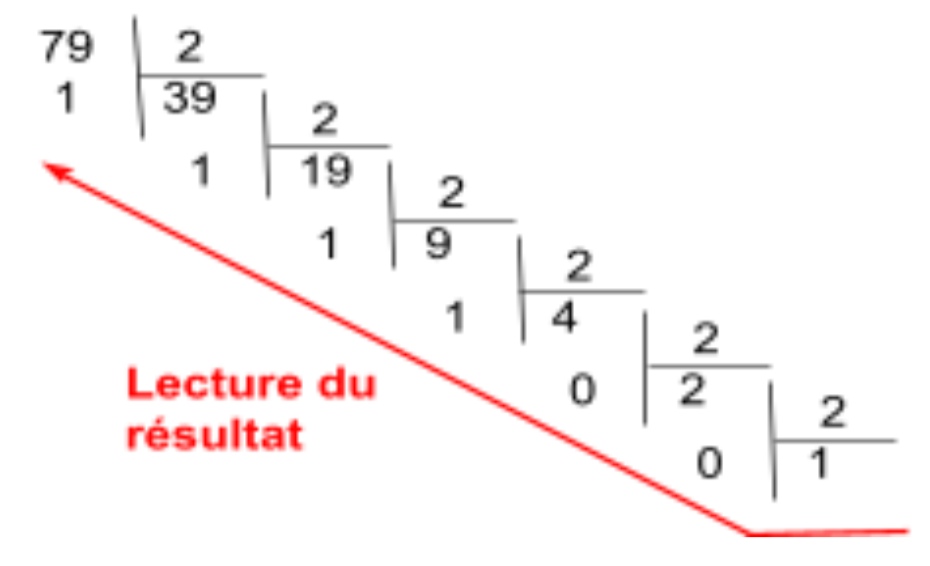
\includegraphics[scale=.5]{Images/intro/divisionbinaire}
	\end{center}
\end{figure}

Ainsi, $79_{(10)}=1001111_{(2)}$

\begin{myexamples}
	\item En binaire, le nombre décimal 10 s'écrit
	\vspace{3cm}
	\item En binaire, le nombre décimal 58 s'écrit
	\vspace{3cm}	
\end{myexamples}

\subsection{La base hexadécimal}
Il 
C'est le code utilisé dans la programmation de certains automates et microprocesseurs. Il est composé de : 10 chiffres de 0 à 9, et 6 lettres de A à F. Les adresse MAC (adresses unique associée à chaque carte réseau dans le monde) sont aussi écrite en base hexadécimal.

La manipulation des nombres écrits en binaire est difficile pour l'être humain et la conversion en décimal n'est pas simple. C'est pourquoi nous utilisons de préférence le système hexadécimal (base 16). 

Le tableau ci-dessous montre la représentation des nombres de 0 à 15 dans les bases 10, 2 et 16.

\begin{figure}[h]
	\begin{center}
		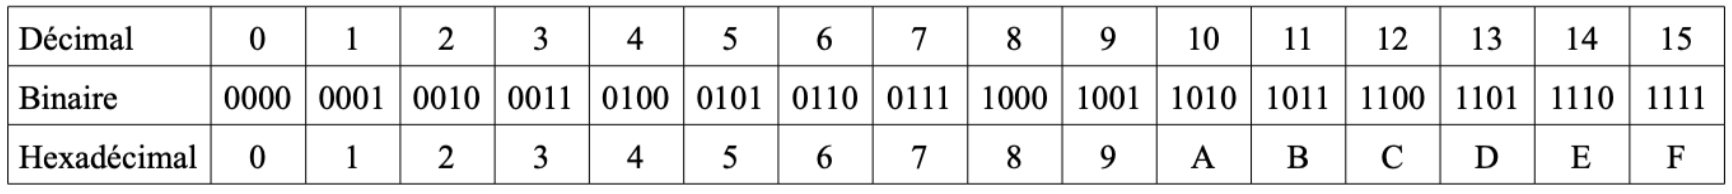
\includegraphics[scale=.5]{Images/intro/tableaubase}
	\end{center}
\end{figure}


Par exemple, $B4F_{(16)}= B \cdot 16^2 + 4 \cdot 16^1 + F\cdot 16^0= 11 \cdot 16^2 + 4 \cdot 16^1 + 15\cdot 16^0=2 895_{(16)}$

\subsubsection{Conversion en binaire}

Pour convertir un nombre binaire en hexadécimal il suffit de remarquer que chaque groupe de 4 bits représentes un chiffre en hexadécimal:

\begin{figure}[h]
	\begin{center}
		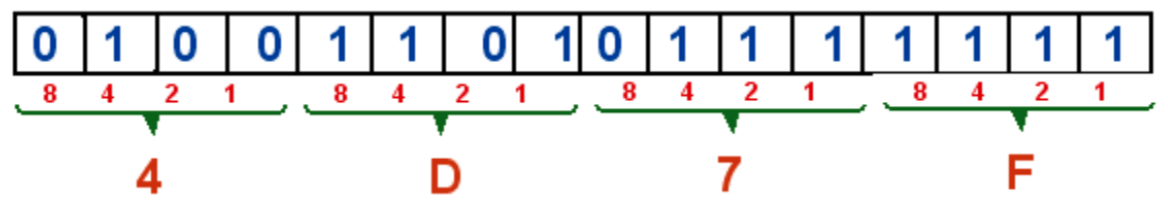
\includegraphics[scale=.5]{Images/intro/hexadecimal}
	\end{center}
\end{figure}

\begin{myexample}
	Le  nombre binaire $101000111100_{(2)}$ s'écrit en base hexadécimal :
	\vspace{2cm}

\end{myexample}

\subsubsection{Conversion en décimal}

La méthodes par divisions (par 16) s'applique comme en binaire (par 2).


\mainsection{\the\numexpr \thechapter + 1 \relax}{Information et donnée}{13/09/2021}


\vspace{-1cm}
\section{Rappel}
\vspace{-0.5cm}
\begin{mydefinition}
	L'{\bf octet} est une unité d'information composée de 8 bits. Il permet par exemple de stocker un caractère comme une lettre ou un chiffre.
\end{mydefinition}
Dans le monde des ordinateurs, les bits sont en général regroupé en \textbf{octet}, c'est-à-dire par paquet de 8. En général, pour faciliter la lecture, on écrit la valeur des octets en hexadécimal plutôt qu'en binaire.
\begin{myexample}
	L'octet  $0011\,1100_{(2)}$ s'écrit en base hexadécimal :
	\vspace{1cm}
	
\end{myexample}


\section{Codage du texte}
La première opération que j'effectue après avoir allumé mon ordinateur est de rentrer mon identifiant avec le bon mon mot de passe. Donc, l'ordinateur doit être capable de traiter du texte et avoir un moyen de représenter ce type de donnée en binaire!

Le binaire nous permet de représenter n'importe quel nombre. Donc, pour représenter du texte, il suffit d'associer à chaque caractère (lettres, symboles de ponctuation, caractère de contrôle) un nombre. 
\subsection{La table ASCII}
  Le premier système de représentation de texte avait été développé dans le but de transmettre des messages vers l'ordinateur. Les données étaient codées sur le système de base, à savoir l'octet. Pour des raisons de fiabilités, seulement 7 des 8 bits de l'octet était utilisé pour codé l'information : 
  \begin{itemize}
  	\item Les 7 premier bits (bits de poids les plus faible) servent à représenter la donnée, ce qui permet de représenter $2^7=128$ nombre, donc 128 caractères possibles. 
  	\item Le dernier bit (bit de poids le plus fort, le plus à gauche) sert à vérifier si la donnée n'a pas été altérée durant la transmission (bit de parité).
  \end{itemize}
  Ces contraintes ont donné lieu à la codification ASCII (American Standard Code for Information Interchange), dans laquelle les caractères les plus usuels sont associés à un nombre en 0 et 127).
   
\newpage

\begin{figure}[h!]
{\scriptsize
\begin{multicols}{2}
		\begin{tabular}{|c|c|c|c|}
			\hline
			Décimal     &Hex  &Binaire   &Caractère\\
			\hline
			0       &00   &00000000      &NUL  \\  
			1       &01   &00000001      &SOH   \\ 
			2       &02   &00000010      &STX    \\
			3       &03   &00000011      &ETX    \\
			4       &04   &00000100      &EOT    \\
			5       &05   &00000101      &ENQ    \\
			6       &06   &00000110      &ACK    \\
			7       &07   &00000111      &BEL    \\
			8       &08   &00001000       &BS    \\
			9       &09   &00001001       &HT    \\
			10      &0A   &00001010       &LF   \\
			11      &0B   &00001011       &VT   \\
			12      &0C   &00001100       &FF   \\
			13      &0D   &00001101       &CR   \\
			14      &0E   &00001110       &SO   \\
			15      &0F   &00001111       &SI   \\
			16      &10   &00010000      &DLE   \\
			17      &11   &00010001      &DC1   \\
			18      &12   &00010010      &DC2   \\
			19      &13   &00010011      &DC3   \\
			20      &14   &00010100      &DC4   \\
			21      &15   &00010101      &NAK   \\
			22      &16   &00010110      &SYN   \\
			23      &17   &00010111      &ETB   \\
			24      &18   &00011000      &CAN   \\
			25      &19   &00011001      &EM   \\
			26      &1A   &00011010      &SUB   \\
			27      &1B   &00011011      &ESC   \\
			28      &1C   &00011100      &FS   \\
			29      &1D   &00011101      &GS   \\
			30      &1E   &00011110      &RS   \\
			31      &1F   &00011111      &US   \\
			32      &20   &00100000      &SP [space]\\
			33      &21   &00100001      &!\\
			34      &22   &00100010      &"\\
			35      &23   &00100011      &\#\\
			36      &24   &00100100      & \$ \\
			37      &25   &00100101      &  \%  \\
			38      &26   &00100110      &  \&  \\
			39      &27   &00100111     &' \\
			40      &28   &00101000     &   ( \\
			41      &29   &00101001      &  ) \\
			42      &2A   &00101010       & * \\
			43      &2B   &00101011        &+ \\
			44      &2C   &00101100        &, \\
			45      &2D   &00101101        &- \\
			46      &2E   &00101110        &. \\
			47      &2F   &00101111        &/ \\
			48      &30   &00110000        &0\\
			49      &31   &00110001        &1\\
			50      &32   &00110010        &2\\
			51      &33   &00110011        &3\\
			52      &34   &00110100        &4\\
			53      &35   &00110101        &5\\
			54      &36   &00110110        &6\\
			55      &37   &00110111        &7\\
			56      &38   &00111000        &8\\
			57      &39   &00111001        &9\\
			58      &3A   &00111010        &:\\
			59      &3B   &00111011        &;\\
			60      &3C   &00111100        &<\\
			61      &3D   &00111101        &=\\
			62      &3E   &00111110        &>\\
			63      &3F   &00111111        &?\\
			\hline
		\end{tabular}

	\begin{tabular}{|c|c|c|c|}
		\hline
		Décimal     &Hex  &Binaire   &Caractère\\
		\hline
64      &40   &01000000        &@\\
65      &41   &01000001        &A\\
66      &42   &01000010        &B\\
67      &43   &01000011        &C\\
68      &44   &01000100        &D\\
69      &45   &01000101        &E\\
70      &46   &01000110        &F\\
71      &47   &01000111        &G\\
72      &48   &01001000        &H\\
73      &49   &01001001        &I\\
74      &4A   &01001010        &J\\
75      &4B   &01001011        &K\\
76      &4C   &01001100        &L\\
77      &4D   &01001101        &M\\
78      &4E   &01001110        &N\\
79      &4F   &01001111        &O\\
80      &50   &01010000        &P\\
81      &51   &01010001        &Q\\
82      &52   &01010010        &R\\
83      &53   &01010011        &S\\
84      &54   &01010100        &T\\
85      &55   &01010101        &U\\
86      &56   &01010110        &V\\
87      &57   &01010111        &W\\
88      &58   &01011000        &X\\
89      &59   &01011001        &Y\\
90      &5A   &01011010        &Z\\
91      &5B   &01011011      &  [ \\
92      &5C   &01011100      &  \char`\\ \\
93      &5D   &01011101      &  \symbol{93}\\
94      &5E   &01011110      &  \symbol{94} \\
95      &5F   &01011111      &  \symbol{95} \\
96      &60   &01100000      &  \symbol{96}\\
97      &61   &01100001      &  a\\
98      &62   &01100010      &  b\\
99      &63   &01100011      &  c\\
100     &64   &01100100      &  d\\
101      &65   &01100101      &  e\\
102      &66   &01100110      &  f\\
103      &67   &01100111      &  g\\
104      &68   &01101000      &  h\\
105      &69   &01101001      &  i\\
106      &6A   &01101010      &  j\\
107      &6B   &01101011      &  k\\
108      &6C   &01101100      &  l\\
109      &6D   &01101101      &  m\\
110      &6E   &01101110      &  n\\
111      &6F   &01101111      &  o\\
112      &70   &01110000      &  p\\
113      &71   &01110001      &  q\\
114      &72   &01110010      &  r\\
115      &73   &01110011      &  s\\
116      &74   &01110100      &  t\\
117      &75   &01110101      &  u\\
118      &76   &01110110      &  v\\
119      &77   &01110111      &  w\\
120      &78   &01111000      &  x\\
121      &79   &01111001      &  y\\
122      &7A   &01111010      &  z\\
123      &7B   &01111011      &  \symbol{123}\\
124      &7C   &01111100      &  \symbol{124}\\
125      &7D   &01111101      &  \symbol{125}\\
126      &7E   &01111110      &  \symbol{126}\\
127      &7F   &01111111      &DEL\\
			\hline
		\end{tabular}

\end{multicols}}
\caption{Table ASCII}
\end{figure}
On remarque que les 32 premiers caractères ne sont pas des symboles à proprement dit, mais plutôt des caractères de contrôle liés, par exemple, à un touche sur le clavier comme ESC ou DEL.
\begin{eclairage}
	Lorsque l'on tape du texte, chaque fois que l'on fait un retour à la ligne avec la touche "Enter" génère habituellement deux codes : un retour chariot et un saut de ligne, qui s'appellent respectivement CR (carriage return, caractère numéro 13 dans la table ASCII) et LF (line feed, caractère numéro 10 dans la table ASCII).

\end{eclairage}
	
\subsection{L'Unicode}
Le code ASCII était à l’origine conçu pour des textes écrits en anglais. Dans un premier temps, la table ASCII a été étendue, en utilisant les 8 bits pour coder d'autres caractères. Cette nouvelle table ASCII, appelée table ASCII étendue, contenait 256 caractères. On y trouve, la plupart des caractère utilisé en français comme les voyelles avec leurs accents ou le "c" cédille "ç".

Compte-tenu  de  l‘extension  mondiale  de  l‘informatique, il s'est rapidement avéré que 256 caractères ne seraient pas suffisant pour écrire en chinois, russe, ... Pour pallier à cette limitation du code ASCII, les  organismes  de  normalisation  ISO  travaillent  depuis 1988 à la création d‘un code universel (UNIversal CODE). Ce code cherche à supprimer les pages de code et à reprendre l'ensemble des caractères utilisés de par le monde. Il reste basé sur la codification ASCII. 

Il se représente sous 3 formes : 
\begin{itemize}
	\item UTF8 étant beaucoup utilisé sur Internet et présentant un codage de taille variable, certain caractère . 
	\item UTF16 de taille fixe sur 2 octets, théoriquement $2^{32}-1 =65'535$ caractères différents.
	\item UTF32 sur 4 octets
\end{itemize}

En  UTF8,  tous  les  caractères  de  base  ASCII  7  bits (le tableau ci-dessus) sont  codés  sur  1  octet.  Au-delà,  les caractères peuvent prendre de 2 à 4 octets. 
\begin{myexample}
	Quelques caractères codé en UTF8\\
	
	\hspace{1cm}
	\begin{tabular*}{14.5cm}{@{\extracolsep{\fill}}  l  l  l }
		é \ \ \ \ \small{C3 A9$_{16}$}  &  \euro \ \ \ \ \small{E2 82 AC$_{16}$}  &  \~ \ \ \ \ \small{7E$_{16}$}  \\
		A \ \ \ \ \small{41$_{16}$}  &  ù \ \ \ \ \small{C3 B9$_{16}$}  & Ê \ \ \ \ \small{C2 8A$_{16}$}   \\
	\end{tabular*}
\end{myexample}



\section{Les images}
Il existe deux familles d'images qui font appel à des représentation très différentes:
\begin{itemize}
	\item \textbf{Les images matricielles} qui sont composées de points appelés pixels que l’on ne discerne pas à l'œil nu. 
	\item Les images vectorielles qui sont composées d'objets géométrique élémentaires comme des droites, segments, cercles, courbes,  etc...
\end{itemize}
Les images vectorielles jouent principalement un rôle dans la création graphique mais leur rôle est moindre dans le processus d'acquisition de l'information via un capteur comme une caméra ou de la restitution d'information via un moniteur comme un écran \footnote{Le cas des imprimantes est moins clair.}. Dans ce chapitre, nous étudierons seulement le cas de la représentation d'images matricielles. 

\subsection{Les images matricielles}
Une \textbf{image matricielle} est constituée d'un tableau de points ou "petit carrés" appelés \textbf{pixels}. Chaque pixel possède une unique couleur. Lorsque la densité de pixel est grande on ne ne perçoit pas les pixels. 
\begin{figure}[h!]
	\centering
	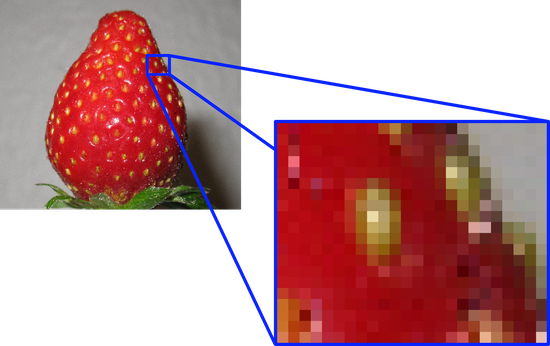
\includegraphics[trim=10 0 0 20,width=0.5\textwidth]{Images/codage_information/Zoom_sur_une_image}
	\caption{Une image préparée pour être affichée sur un écran est "découpée" en un tableau de pixels ayant chacun une couleur donnée.}
\end{figure}
Le codage d'image est un entreprise autrement plus complexe que le codage de texte. Commençons par une image en noir et blanc, dans ce cas chaque pixel est soit blanc, soit noir. Par conséquent le codage le plus simple est de représenter chaque pixel avec un 1 ou un 0. 

\begin{figure}[h!]
	\centering
	\subfloat{%
		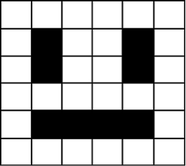
\includegraphics[trim=0 0 0 0,width=0.3\textwidth]{Images/codage_information/img_bin1}
	}
	\hspace{1cm}
	\subfloat{%
		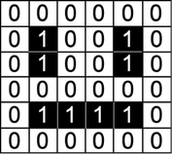
\includegraphics[trim=0 0 0 0,width=0.3\textwidth]{Images/codage_information/img_bin2}
	}
	\hspace{1cm}
	\subfloat{%
	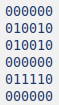
\includegraphics[trim=0 0 0 0,width=0.15\textwidth]{Images/codage_information/img_bin3}
	}
	\caption{Représentation d'une image binaire}
	\label{img_bin}
\end{figure}
Si on reprend l'exemple de la figure \ref{img_bin}, notre image pourrait être représentée par la suite de bits:\\
\hspace{1cm} 000000010010010010000000011110000000.\\
Cependant dans ce cas là, il faut aussi spécifier les dimensions de l'image pour que le codage soit complet (6 x 6 ici). On appelle ces données, les \textbf{méta-données}.
%\begin{mydefinition}
%	Les méta-données sont les données nécessaire à la reconstruction de l'
%\end{mydefinition}
	
\subsection{image en niveau de gris}
La vie est faite de nuance et les images en noir et blanc n'échappe pas à ce constat, il existe plusieurs nuances de gris entre le blanc et le noir. En général, ces niveaux de gris sont codés avec un octet ce qui permet 255 nuances entre le noir (codé avec nombre 0) et le blanc (codé avec le nombre $255=11111111_2$).

\begin{figure}[h!]
	\centering
	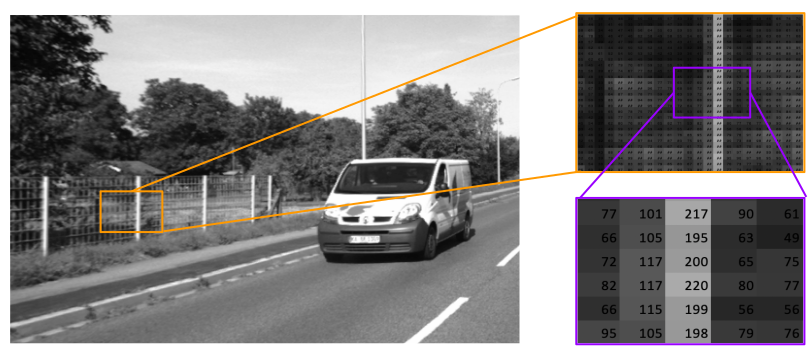
\includegraphics[trim=10 0 0 20,width=0.8\textwidth]{Images/codage_information/image_gris.png}
	\caption{Codage d'une image en niveau de gris. Chaque pixel est associé à un nombre entre 0 et 255 qui . Le nombres sur les pixels représentent l'intensité du niveau de gris, cette indication n'existe pas sur l'image d'origine (\textit{source: Informatique au gymnase}).}
\end{figure}

\subsection{Codage des couleurs*}
Les pixels de la plupart des écrans d'ordinateur sont composés de 3 "lampes" : une rouge, une verte et une bleue.

\begin{figure}[h!]
	\centering
	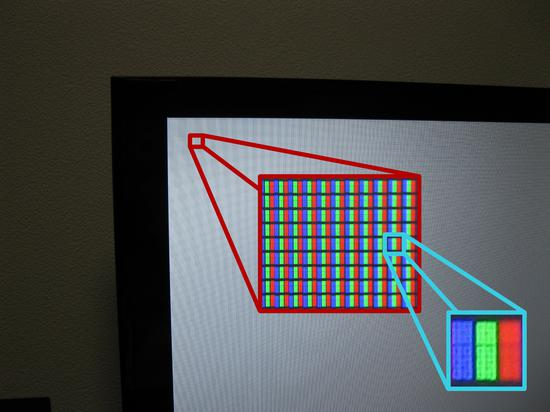
\includegraphics[trim=0 0 60 0,width=0.5\textwidth]{Images/codage_information/Zoom_sur_un_pixel.jpg}
	\caption{Zoom sur un pixel. On peut voir les pixels d'un écran en se rapprochant très près de celui-ci, ou avec une loupe (source: \textit{science-questions.org}).}
\end{figure}

\begin{wrapfigure}[]{r}{0.3\textwidth}
	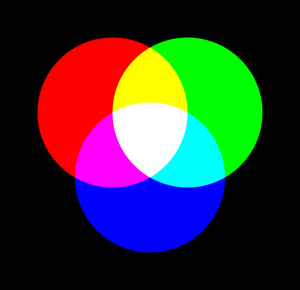
\includegraphics[trim=0 0 0 20,width=0.28\textwidth]{Images/codage_information/Addition_des_couleurs.png}
\end{wrapfigure}

\textit{Les pixels utilisent ainsi des propriétés d'additivité des couleurs qui permettent, à partir de trois couleurs, de générer un arc-en-ciel de couleurs du rouge au violet. Pour déterminer quelle couleur est obtenue en fonction des lumières allumées, on peut s'aider du schéma ci-dessous qui représente la superposition de trois projecteurs, rouge, vert et bleu (source: science-questions.org):}

%\begin{figure}[h!]
%	\centering
%	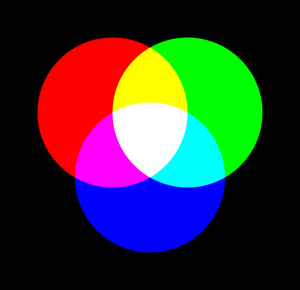
\includegraphics[trim=10 0 0 0,width=0.3\textwidth]{Images/codage_information/Addition_des_couleurs.png}
%	\caption{Addition des couleurs}
%\end{figure}
Pour le codage des images couleurs, on codera chaque pixel en utilisant 3 octets, ce qui donne
\begin{itemize}
	\item R: 255 nuance de rouge,
	\item G: 255 nuance de vert,
	\item B: 255 nuance de bleu.
\end{itemize}

\begin{figure}[h!]
	\centering
	\subfloat[Image originale]{%
		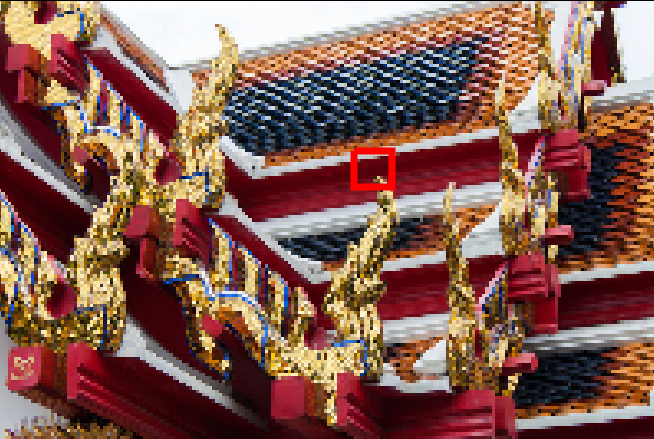
\includegraphics[trim=0 0 0 0,width=0.5\textwidth]{Images/codage_information/image_couleur}
	}
	\hspace{1cm}
	\subfloat[Zoom sur des pixels avec leurs valeurs RGB]{%
		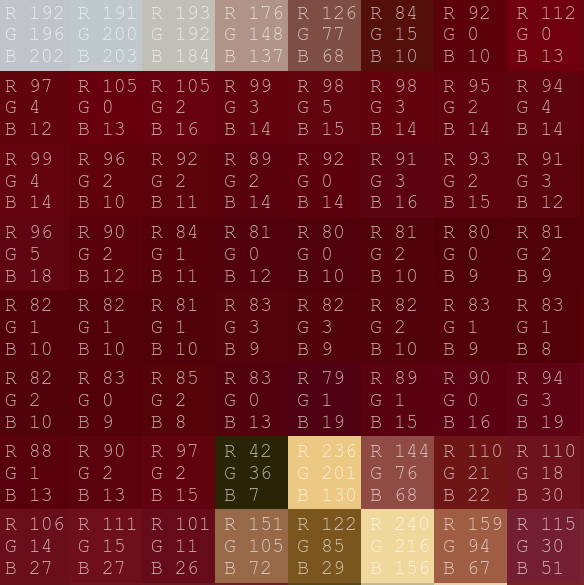
\includegraphics[trim=0 0 0 0,width=0.33\textwidth]{Images/codage_information/image_couleur_zoom}
	}
	\caption{chaque pixel d'une image est représenté avec 3 intensités de rouge(R), vert(G) et bleu(B) allant de 0 à 255 (codé chacune avec 1 octet).}
	\label{img_coul}
\end{figure}


\section{*Sons}
Sans empiéter dur le cours de physique, les sons peuvent être modélisés comme des signaux variant au cours du temps. Ces signaux sont converties sous forme des nombres à travers un processus comme appelle échantillonnage qui va déterminer les temps auquel on mesure le signaux et les différents niveaux d'intensité que sont possibles (ces niveaux sont codés en binaire).

\begin{figure}[h!]
	\centering
	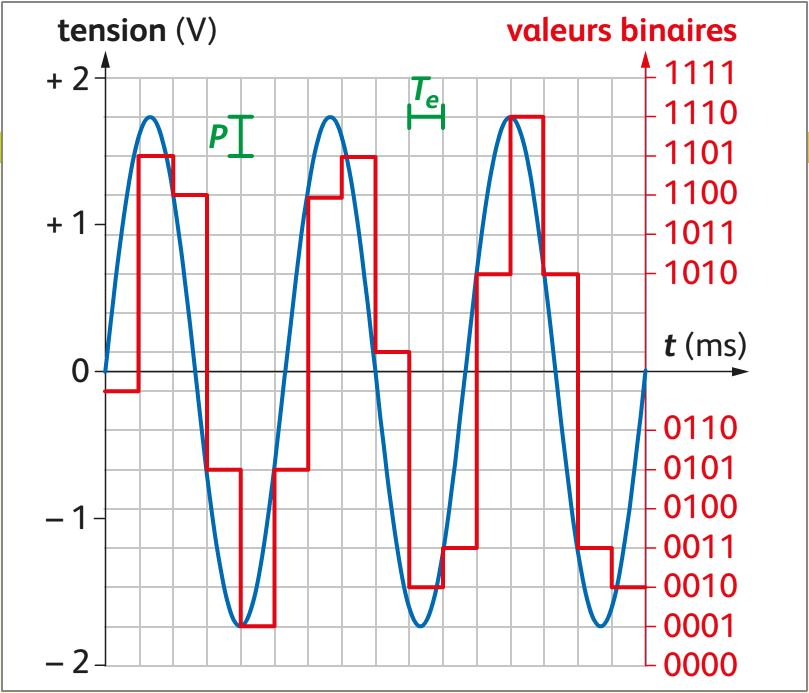
\includegraphics[trim=10 0 60 0,width=0.5\textwidth]{Images/codage_information/illustration_echantillonage.jpg}
	\caption{Exemple de numérisation d'un signal.}
\end{figure}
\vspace{-0.5cm}
\section{*Vidéos}
Les vidéos peuvent être représentées comme une succession d'image (par exemple, autour de 24  images par secondes afin que l’œil ne puisse pas distinguer les images qui défilent) associé avec du son. 
\mainsection{\the\numexpr \thechapter + 1 \relax}{L'ordinateur}{20/09/2021}

%Théorie :
%Identifier le rôle des composants principaux d’un ordinateur.
%
%Pratique :
%Comprendre un catalogue de vente. Être capable de comparer deux machines. 
%(à distiller sur l’année lorsque le moment est favorable ou que cela s’intègre naturellement de nos séquences) 
\section{Les fondamentaux de l'ordinateur}
Un ordinateur peut être décrit comme une machine qui permet d'automatiser le traitement "d'informations" en suivant  des programmes constitués de suites d’opérations arithmétiques et logiques. En particulier, un ordinateur est capable d’acquérir de l’information, de la stocker, de la transformer et de la restituer sous une autre forme. On retrouvera toujours les ingrédients suivants
\begin{itemize}
	\item entrées/sorties, qui permettent à l'ordinateur de communiquer avec l'extérieur ;
	\item une mémoire qui mémorise les données à manipuler ;
	\item un processeur, qui manipule l'information et donne un résultat.
\end{itemize}

\begin{figure}[h!]
	\centering
	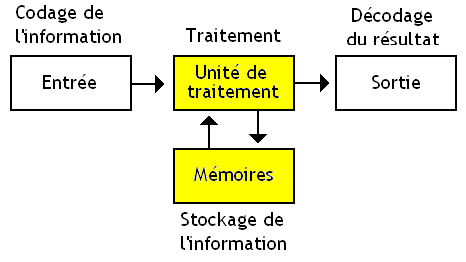
\includegraphics[trim=10 0 20 0,width=0.5\textwidth]{Images/ordinateur/Architecture_Von_Neumann_basic.png}
	\caption{Architecture d'un système à mémoire (\textit{source: https://fr.wikibooks.org/}).}
\end{figure}

\subsection{L'architecture de Von Neumann}
Jusque dans les années 40, les premiers ordinateurs étaient construits dans le but d'accomplir une tâche bien spécifique en suivant un unique programme. En 1940, le mathématicien John von Neumann imagina un type d'architecture novatrice qui permettait une programmation de la machine bien plus souple. Il eu l'idée génial d'imaginer que la mémoire pourrait servir à stocker, en plus des donnés, les instructions du programme lui même. Une telle architecture, dite de Von Neumann, décompose l’ordinateur en trois parties distinctes:
\begin{itemize}
	\item Le \textbf{processeur} qui est composé 
	\begin{itemize}
		\item d’une \textbf{unité arithmétique} et logique (UAL ou ALU en anglais) ou unité de traitement. Son rôle est d’effectuer les opérations de base (addition, multiplication, comparaison,...);
		\item  d’une \textbf{unité de contrôle} qui est chargée du séquençage des opérations du programme ;
	\end{itemize}
	\item La mémoire qui contient à la fois les données et le programme exécuté par l’unité de contrôle. La mémoire se divise entre
	 \begin{itemize}
	 	\item \textbf{mémoire vive ou RAM} (Random Access Memory) qui contient programmes et données en cours de traitement, 
	 	\item \textbf{mémoire permanente ou morte} qui stocke les programmes et données de base de la machine ;
	\end{itemize} 	
	\item Les dispositifs d’entrée-sortie, qui permettent de communiquer avec le monde extérieur.
\end{itemize}
\begin{figure}[h!]
	\centering
	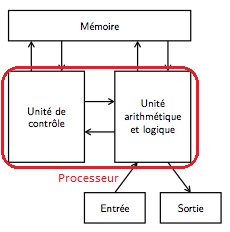
\includegraphics[trim=0 0 0 0,width=0.45\textwidth]{Images/ordinateur/arse1_archi_von_neumann_sans_accu.png}
	\caption{Architecture de Von Neumann (\textit{source: https://fr.wikibooks.org/}).}
\end{figure}

La circulation de l’information entre ces différents éléments (représentée par des flèches sur le schéma ci-dessus) est assurée par des connexions appelées \textbf{bus} (bus de données, bus d’adresse, bus de signal lecture/écriture...). Il s’agit tout simplement de fils électriques utilisés pour transmettre de données binaires.
\begin{mydefinition}
	Un \textbf{bus} informatique désigne l'ensemble des lignes de communication connectant les différents composants d'un ordinateur.
\end{mydefinition}


\subsection{Le processeur}
Le processeur, (ou CPU, Central Processing Unit, "Unité centrale de traitement" en français) est le composant essentiel d’un ordinateur qui interprète les instructions et traite les données d’un programme.
Le processeur est un circuit électronique complexe (circuit intégré) qui exécute chaque instruction très rapidement, en quelques cycles d’horloges. Toute l’activité de l’ordinateur est cadencée par une horloge unique, de façon à ce que tous les circuits électroniques travaillent tous ensemble de façon synchronisée. La fréquence de
cette horloge s’exprime en MHz (millions de cyles par seconde) ou GHz (milliards de cycles par secondes). 
\begin{important}
	Le processeur dispose d'une \textbf{horloge} (clock en anglais)  qui cadence l'exécution des instructions. L'unité est appelée \textbf{cycle}. La vitesse de cette horloge ce mesure en Hz, c'est-à-dire en nombre d'instructions exécutées en une seconde. La vitesse de l'horloge est une des caractéristiques principales pour mesurer la performance d'un processeur.
\end{important}

\begin{myexamples}
	\item le processeur de l'Iphone 13, le “Apple A13 Bionic" possède une horloge cadencée à 2,65 GHz, c'est-à-dire 2,65 milliards d'opérations par seconde.
	\item le processeur qui équipe la dernière génération de HP G4 (les PCs de la salle de cours) sont des Intel Xeon W-2225, des processeurs avec une horloge cadencée à 4,10 GHz, c'est-à-dire 4'100'000'000 opérations par seconde. 
\end{myexamples}
	
\begin{eclairage}
	Jusqu'en 2004 environ, la fréquences des ordinateurs a augmenté de manière exponentielle. Depuis elle stagne. En effet, au-delà d'une certaine fréquence il devient très difficile de dissiper la chaleur produite par le processeur ce qui perturbe la lecture des signaux électriques lus aux bornes du processeur voire détériorer le circuit électrique eu même.
	\begin{center}
		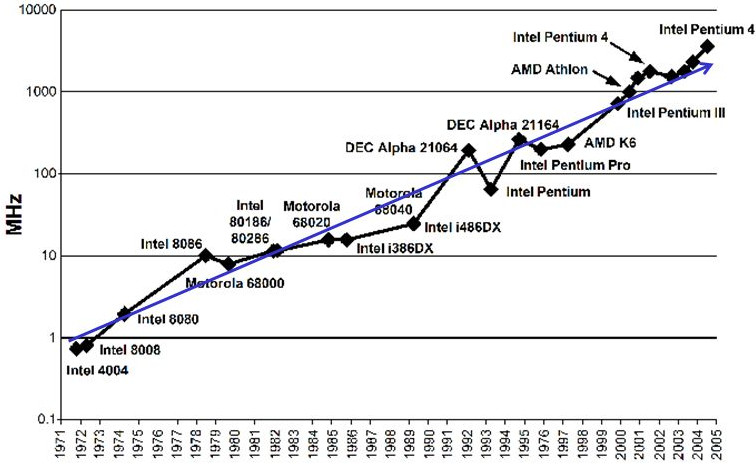
\includegraphics[trim=0 0 0 0,width=0.6\textwidth]{Images/ordinateur/evolution_frequence_ordinateur.jpg}
	\end{center}
\end{eclairage}
Pour chaque instruction,  le processeur effectue schématiquement (de manière simplifié) les opérations suivantes :
\begin{enumerate}
	\item lire dans la mémoire principale l’instruction à exécuter ;
	\item effectuer le traitement correspondant à cette instruction ;
	\item passer à l’instruction suivante.
\end{enumerate}
\begin{eclairage}
	L'architecture de Von Neumann décrit le fonctionnement de base d'un ordinateur mais c'est une simplification.  comparé celle des ordinateurs d'aujourd'hui. Par exemple,
	\begin{itemize}
		\item les entrées et sorties, initialement commandées par l’unité de contrôle du processeur, sont le plus souvent sous le contrôle (du moins partiellement) de processeurs autonomes. C’est le cas par exemple des cartes graphiques chargées de produire une image sur un écran ou des cartes sons;
		\item les ordinateurs comportent maintenant des processeurs multiples, qu’il s’agisse d’unité séparées ou de
		« cœurs » multiples à l’intérieur d’une même puce. Cette organisation permet d’atteindre une puissance
		globale de calcul élevée sans augmenter la vitesse des processeurs, limitée par les capacités d’évacuation
		de la chaleur.
	\end{itemize}	
\end{eclairage}

\newpage
\subsection{Mémoire}
\begin{wrapfigure}[]{r}{0.4\textwidth}
	\centering
	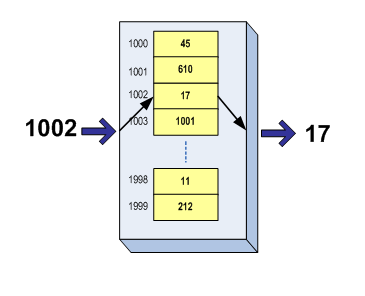
\includegraphics[trim=0 0 0 0,width=0.45\textwidth]{Images/ordinateur/adressage_memoire.png}
	\caption{Accès à la donnée "17" qui se trouve à l'adresse "1002" de la mémoire. (\textit{source: https://fr.wikibooks.org/}).}
\end{wrapfigure}
La mémoire\footnote{Ici on parle de mémoires adressables. La plupart des processeurs possèdent aussi des mémoire internet très rapide qu'on appelle \textbf{mémoire cache}.} peut être vue comme un tableau dans lequel chaque cellule est numérotée par une adresse et qui permet de stocker aussi bien les données que les programmes eux-mêmes.
%\begin{figure}[h!]
%	\centering
%	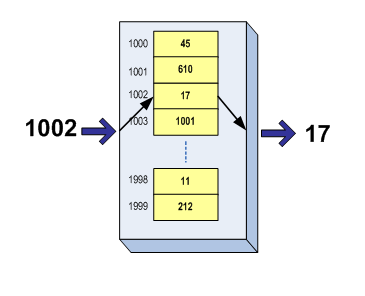
\includegraphics[trim=0 0 0 0,width=0.45\textwidth]{Images/ordinateur/adressage_memoire.png}
%	\caption{Accès à la donnée "17" qui se trouve à l'adresse "1002" de la mémoire. (\textit{source: https://fr.wikibooks.org/}).}
%\end{figure}

On distingue les mémoires en fonction de leur performance (rapidité, fiabilité, durabilité, ... ) mais surtout en fonction de leur usage:
\begin{enumerate}
	\item \textbf{La mémoire vive ou volatile} sert au stockage \textbf{temporaire} des données. Elle doit être \textbf{rapidement accessible} autant pour lire que pour stocker une donnée. En général, la technologie employée s'appuie sur des composants électroniques qui conservent les données seulement si elles sont alimentées en électricité, par conséquent, lorsque l'\textbf{ordinateur est s'éteint les données sont perdues}. \\
	\textbf{Remarque} : L'acronyme anglais RAM (Random Access Memory) est souvent utilisé pour parler de mémoire vive.
	\item \textbf{La mémoire morte} sert au stockage \textbf{persistant} des données. Lorsque l'\textbf{ordinateur est éteint les données sont conservées}.
\end{enumerate}


\begin{eclairage}
 Le processeur accède à la mémoire via des bus. Un bus est constitué d'un ensemble de fils électriques qui permettent de transmettre de l'information binaire entres plusieurs éléments de l'ordinateur. Trois bus permettent au processeur d'échanger avec la mémoire:
 \begin{enumerate}
 	\item Le \textbf{bus d'adressage} qui permet d'indiquer à la mémoire la position de la case de la mémoire qu'on souhaite accéder. Cette position est codée au moyen d'une adresse qui n'est autre qu'un nombre codé en binaire.
 	\item Le bus de données qui permet de communiquer une donnée du processeur à la mémoire (mode écriture) ou de la mémoire vers le processeur (mode lecture)
 	\item Le \textbf{bus de contrôle} qui permet, par exemple, de spécifier le mode de fonctionnement:
 		\begin{enumerate}
 			\item \textbf{mode écriture}: la donnée sur le bus est utilisé pour modifier une espace mémoire à une adresse donnée
 			\item \textbf{mode lecture}: la mémoire transmet au processeur via le bus la donnée à l'adresse demandée.
 		\end{enumerate}
 \end{enumerate}
\begin{center}
	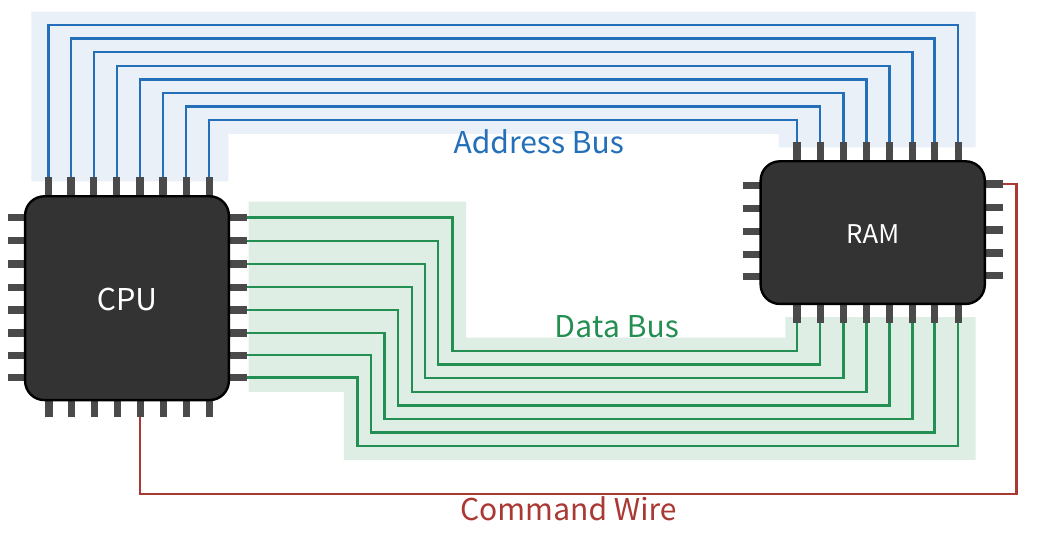
\includegraphics[trim=0 0 0 0,width=0.6\textwidth]{Images/ordinateur/cablage_memoire.png}
\end{center}
\end{eclairage}


\begin{important}
	La mémoire est principalement caractérisée par sa capacité de stockage et sa rapidité d'accès en lecture et en écriture. La capacité de stockage se mesure au nombre d'octets\footnote{Rappel: Un octet correspond à 8 bits} que la mémoire peut stocker. La vitesse se mesure en nombre d'octets par seconde qu'il est possible d'écrire ou de lire sur la mémoire.
\end{important}
\begin{myexample}
	Une clé USB de 4Go peut stocker 4 milliards d'octets, c'est à dite 32 milliards de bits.
\end{myexample}
 
\subsection{Les entrées / sorties}
Les communication avec le monde extérieur se font pas l'intermédiaire de périphérique d'entrées /sorties. Les mots entrée et sortie doivent êtres interprétés du point de vue de l'ordinateur: les entrée c'est qu'il reçoit, les sorties c'est ce qu'il renvoie.

\subsubsection{Les entrées}
L’acquisition de l’information se fait par l’intermédiaire de périphériques d’\textbf{entrées} que sont le clavier, la souris, le micro, la caméra, le scanner, l’écran tactile,... Le point commun entre tous les périphériques d'entrée est qu'ils convertissent l'information qu'ils récupèrent de l'extérieur en données compréhensibles par l'ordinateur (voir les chapitres \ref{codageNombre} et 2).

\subsubsection{Les sorties}
La restitution de l’information se fait par l’intermédiaire de périphériques de \textbf{sorite} que sont l'écran, les écouteurs, l'imprimante,... Ils décodent l'information fournie par l'ordinateur afin de la rendre compréhensible par l'utilisateur (le plus souvent sous forme de textes, images ou sons).

\section{Les ordinateurs d'aujourd'hui}
\begin{wrapfigure}[]{r}{0.45\textwidth}
	\centering
	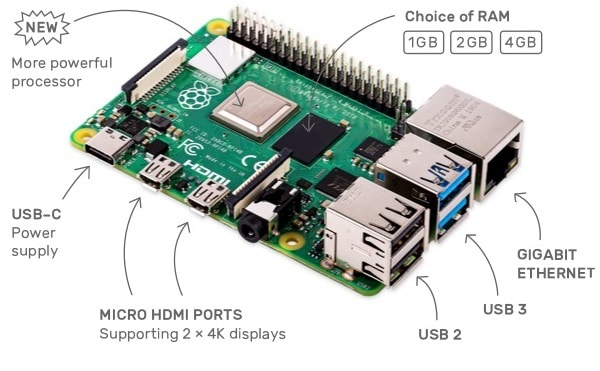
\includegraphics[trim=0 0 0 120,width=0.5\textwidth]{Images/ordinateur/raspberry-pi-4-caracteristiques.jpg}
	\caption{\small Un RaspberryPi 4 .}
\end{wrapfigure}
Nous sommes entouré d'ordinateurs. Par exemple, aujourd'hui vous avez sûrement consulté les écrans d'affichage du collège qui fonctionnent avec un \textbf{Raspberry Pi} (qui est nano-ordinateur monocarte) en se connectant sur un serveur internet. Vous avez aussi probablement consulté votre smartphone (l'ordinateur le plus populaire du monde \footnote{ \url{https://www.numerama.com/tech/722898-le-smartphone-est-lordinateur-le-plus-populaire-au-monde.html}})
et finalement vous allez utiliser un PC (Personnal Computer), ou ordinateur personnel, pendant le cours d'informatique.
\newpage

\section{Le PC}
Le terme \textbf{PC} (Personnal Computer) ou ordinateur personnel désigne un ordinateur qui répond aux besoins des utilisateurs humains et qui est de dimension raisonnable, c'est-à-dire qu'il peut tenir sur un bureau. On parle aussi de micro-ordinateur ou ordinateur individuel. 



\subsection{Les composants  d'un PC}
La carte mère (1) qui est le circuit imprimé \footnote{Le circuit imprimé est un support, en général une plaque, permettant de maintenir et de relier électriquement un ensemble de composants électroniques entre eux.} qui supporte et relie tous les composants propres et les périphériques propres de l'ordinateur. Elle permet de prendre en charge la mémoire vive (4), la lecture du disque dur (7) et l'utilisation du processeur. Cette carte mère est fixée à l'unité centrale également nommée : la tour, le boîtier, desktop, etc.

\begin{center}
	\begin{figure}[h]
		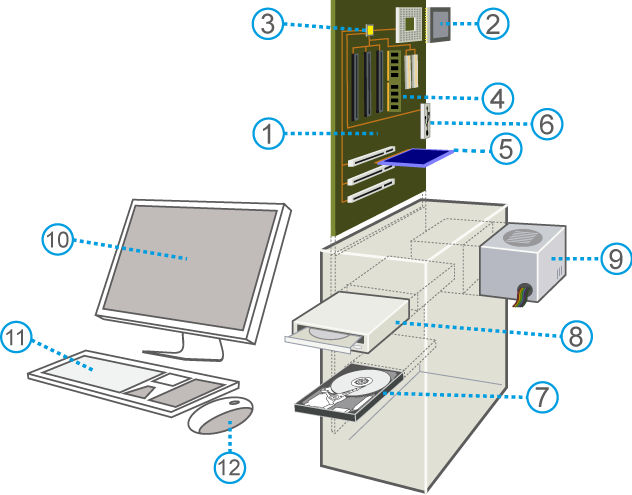
\includegraphics[scale=.6]{Images/ordinateur/composants}
		\caption{L'ordinateur, l'unité centrale et sa composition}
		\label{composants}
	\end{figure}
\end{center}

Les principaux composants constituant un ordinateur sont :
\begin{itemize}%[label=\textbullet]
	\item Le {\bf processeur} (CPU, Central Processing Unit) (2): qui est l'élément central de la carte mère.
	
	\item  La {\bf mémoire vive} (RAM) (4) : qui est sous la forme de une ou plusieurs barrettes qui se fixent à la carte mère.

	\item La {\bf mémoire permanente}: qui était le plus souvent sous la forme de disque dur optique (hard drive, 7) mais qui tend à être remplacé par des disques électronique1 de type SSD (de l'anglais \textit{solid-state drive}).
	
	\item  Le {\bf lecteur/graveur CD/DVD/Blu-ray } (8) : qui il lit l'ensemble des CD, DVD et Blu-ray, que ce soit de la musique, des logiciels, des jeux, des films, etc. Son utilisation par défaut tend à disparaître.
	
	\item L'{\bf alimentation} (9) : branchée sur le réseau électrique 220 [V], elle alimente tous les composants électroniques.
	
	\item La {\bf carte graphique} (graphic card) (5) : elle transmet les images qu'elle possède en mémoire sur les écrans. Elle permet donc d'afficher à l'écran des images, du texte, des vidéos, etc. en allumant des points lumineux (pixels). À noter que certains processeurs comportent une unité graphique rendant obsolète l'ajout d'une carte graphique sur un ordinateur, typiquement pour un usage de type bureautique.
\end{itemize}


\subsection{Caractéristiques détaillés des composants}


\subsubsection{La carte mère}
\begin{wrapfigure}[]{r}{0.4\textwidth}
\centering
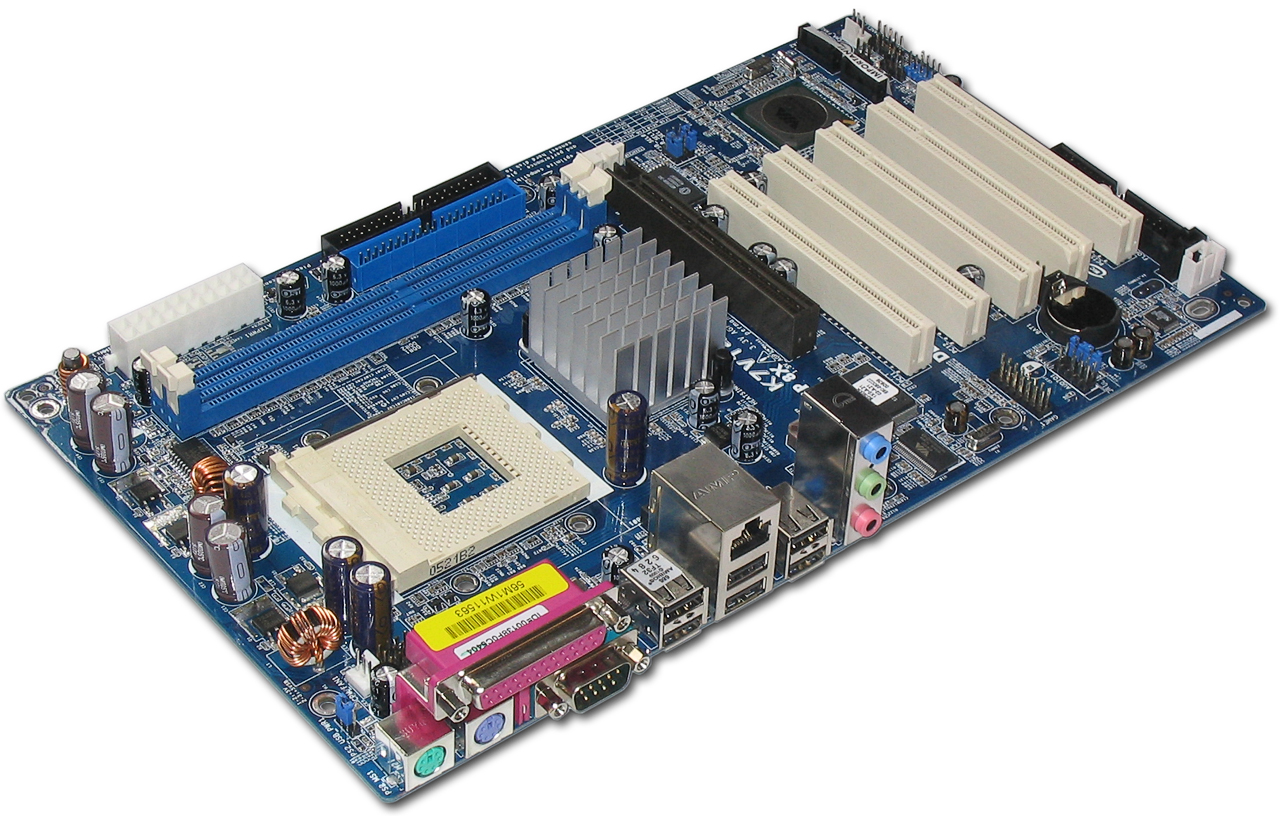
\includegraphics[trim=0 0 0 000 ,scale=.4]{Images/ordinateur/cartemere}
\caption{Carte mère d'un PC}
\end{wrapfigure}
Une {\bf carte mère} se distingue principalement par la génération de processeur qu'elle peut accueillir, par le type de mémoire vive pouvant être connecté, le nombre et les différents types de connecteurs (6) (IDE, sata, PCI, etc.) qu'elle comporte  et par son jeu de composants électroniques (chipset) lui permettant de gérer l'échange de données entre les disques, la mémoire, la carte graphique et les différents périphériques externes d'entrée/sortie. La carte mère comporte également un ensemble de fonctions nommé BIOS ({\it Basic Input Output System}) ou plus récemment UEFI ({\it Unified Extensible Firmware Interface}) lui permettant, lors de sa mise sous tension, d'identifier le matériel connecté sur la carte mère.



\subsubsection{Processeur}
\begin{wrapfigure}[]{r}{0.4\textwidth}
	\centering
	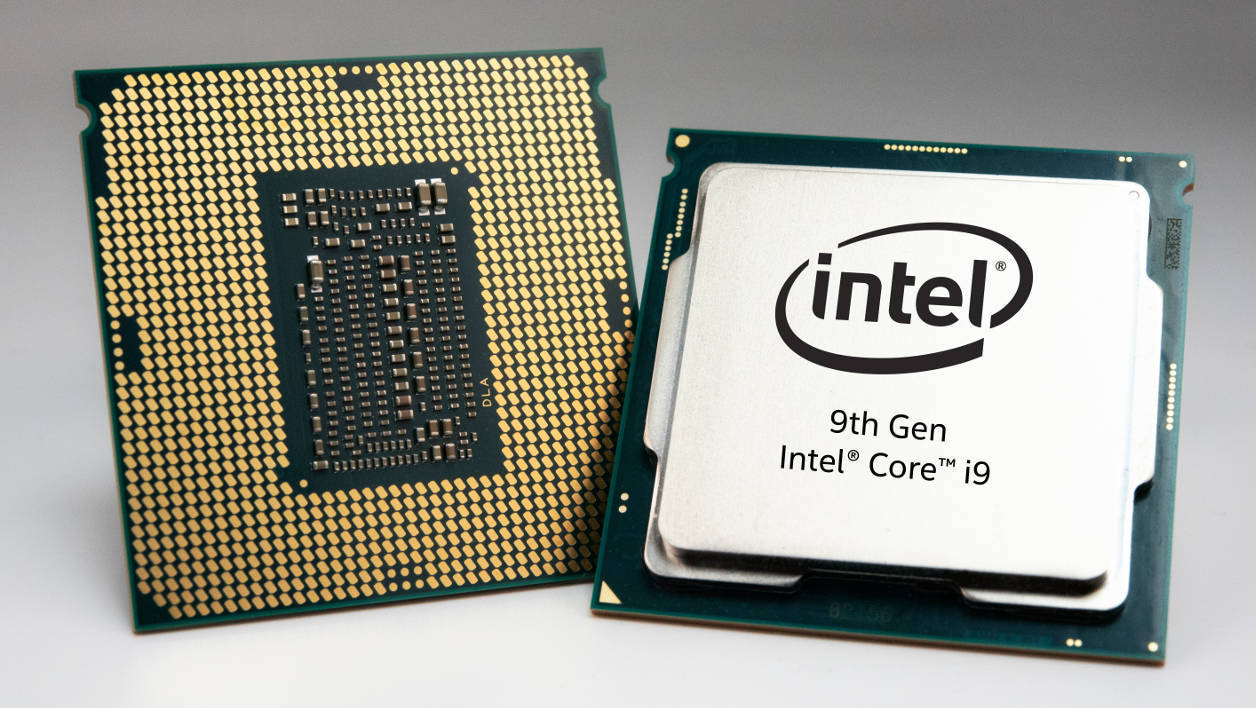
\includegraphics[trim=0 0 0 400 ,width=0.4\textwidth]{Images/ordinateur/processeur}	\caption{Un processeur Intel i9}
\end{wrapfigure}
Un processeur se distingue principalement par sa fréquence de fonctionnement et son architecture (nombre de cœurs, mémoire cache, ...). À l’heure actuelle, la fréquence des PCs varie de 2GHz à 4GHz. Les deux plus important fabricants de processeur de PCs sont Intel et AMD.


\subsubsection{Mémoire}
Qu'il s'agisse de {\bf mémoire vive (RAM)} ou {\bf mémoire permanente}, la mémoire est principalement caractérisée par sa capacité de stockage et sa rapidité d'accès en lecture et en écriture. Actuellement, sa capacité est traduite en gigaoctets [Go] ou téraoctets [To]. La vitesse de lecture et d'écriture est donnée en Mo/s (megaoctets par seconde).
%\begin{figure}[h!]
%	\centering
%	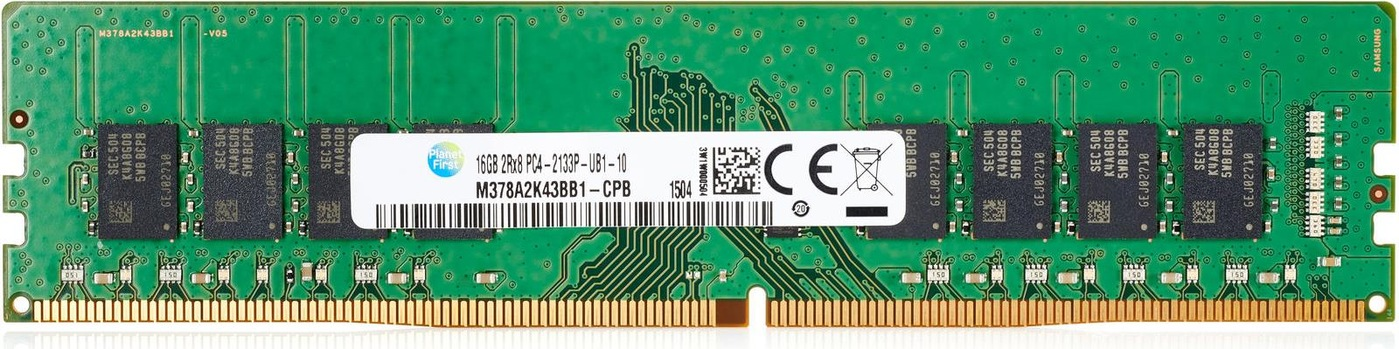
\includegraphics[scale=.2,trim=0 0 0 0]{Images/ordinateur/sdram.jpg}
%	\caption{barrette de RAM}
%\end{figure}
\begin{figure}[h!]
	\centering
	\subfloat[barrette de RAM]{%
		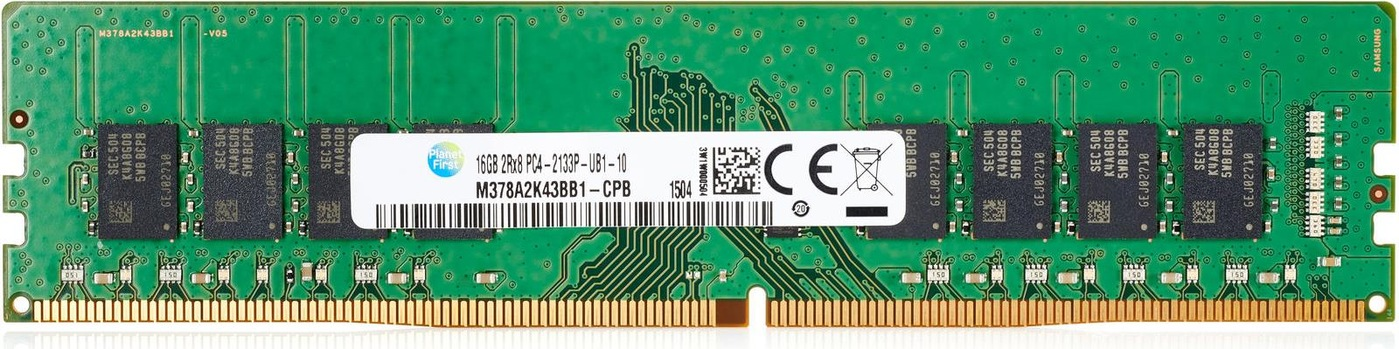
\includegraphics[width=0.5\textwidth,trim=0 0 0 60]{Images/ordinateur/sdram.jpg}
	}
	\hspace{1cm}
	\subfloat[Disque dur]{%
		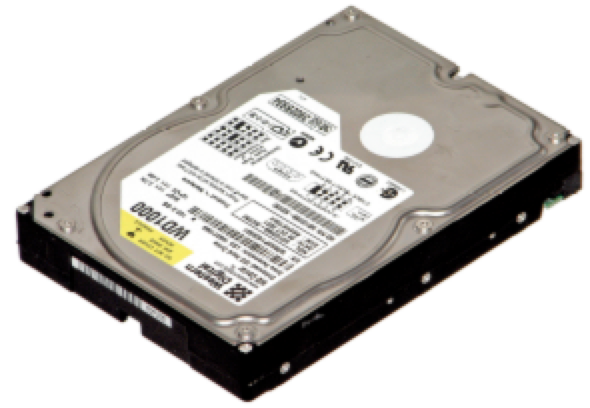
\includegraphics[width=0.3\textwidth,trim=0 0 0 60]{Images/ordinateur/disquedur}
	}
	\caption{Mémoire vive et morte.}
	\label{img_coul}
\end{figure}

\subsubsection{La carte graphique}
\begin{wrapfigure}[]{r}{0.4\textwidth}
	\centering
	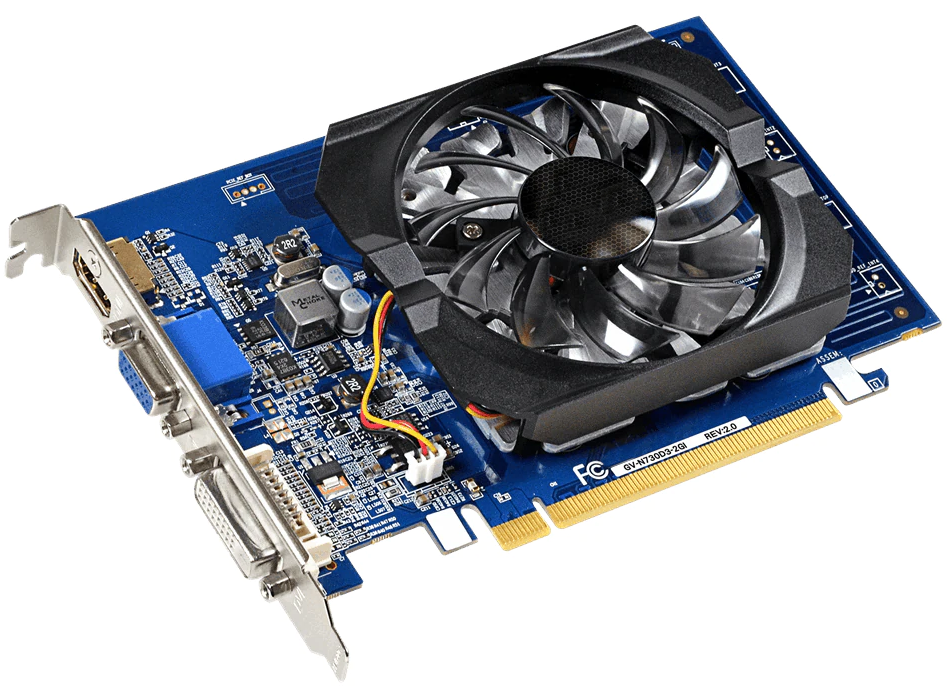
\includegraphics[scale=.2,trim=0 0 0 200]{Images/ordinateur/carte_graphique}
\end{wrapfigure}
La {\bf carte graphique} se caractérise principalement par l'architecture de son processeur graphique (GPU) et sa mémoire vive. À ce jour, Nvidia et AMD sont leaders dans la conception des processeurs graphiques. On distingue très facilement les cartes graphiques les plus puissantes par le système de refroidissement qu’elle possède.





\section{Périphériques externes}

\subsection{Exemples de périphériques}

Pour interagir avec l’ordinateur, des périphériques d’entrée/sortie sont nécessaires. Il en existe de toutes sortes et ces derniers sont connectés à l’ordinateur par différent type de câbles (réseau, USB, DVI, série, etc.) ou à l’aide d’une connexion sans fils (infrarouge, wifi, Bluetooth, lasers, etc).

\begin{figure}[h]
	\centering
	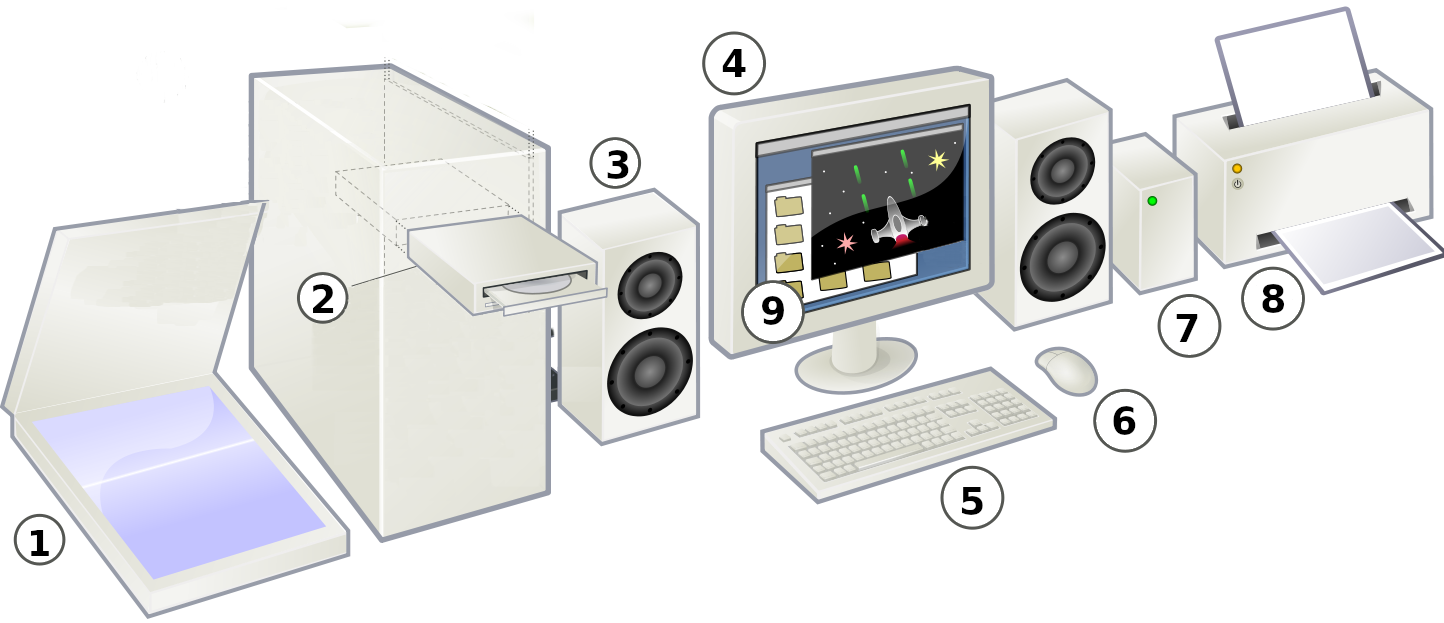
\includegraphics[scale=.3]{Images/ordinateur/peripherique}
	\caption{Périphériques d'un ordinateur}
\end{figure}


Les différents types de périphériques externes sont :
\begin{enumerate}
	\item Le {\bf scanner} permet la numérisation de document dans une certaine résolution.
	\item Le {\bf lecteur} CD ou DVD ou Blu-ray sont des lecteurs permettant de lire un support amovible à l’aide d’un faisceau laser.
	\item Le {\bf haut-parleur} permet de diffuser du son.
	\item L’{\bf écran} permet d’afficher les informations, mais lorsqu’il est tactile, il offre la possibilité de se passer de la souris et du clavier. Il est caractérisé par sa taille et sa définition1 d’écran qui est le nombre de points ou pixels que peut afficher un écran. Actuellement, les définitions (nombre de points H x V) les plus courantes sur un écran pour ordinateur sont :
	\begin{itemize}
		\item XGA : 1024 x 768
		\item  HD : 1280 x 768
		\item  Full HD : 1920 x 1080
		\item WUXGA : 1920 x 1200
		\item  WQHD : 2560 x 1440
		\item 8K Full Format : 8192 x 4320
	\end{itemize}
	\item le {\bf clavier} utilisé pour écrire, mais également se déplacer rapidement dans un texte ou dans des menus voir même effectuer une copie d’écran (screenshot).
	\item La {\bf souris} sert à déplacer le curseur sur l’écran, de choisir des applications et aussi de cliquer sur des icônes pour démarrer des logiciels. Elle permet de naviguer sur votre ordinateur, mais également de dessiner, sélectionner des textes, etc. Elle est mobile avec ou sans fil.
	\item Le {\bf disque externe} est un disque dur qui n’est pas intégré dans l’ordinateur. En fonction de sa taille, il peut être facilement déplacé. En fonction du modèle, les disques externes sont soit alimentés par un branchement USB, soit avec une alimentation sur secteur 220[V].
	\item L’{\bf imprimante} 2D permet l’impression de texte, image, graphique. Il existe plusieurs technologies d’impressions telles que laser, jet d’encre, sublimation, etc. Depuis les années 2010, l’impression 3D prend de l’ampleur avec l’arrivée de nouvelles technologies innovantes basées sur de nouveaux matériaux comme le plastique, la cire, le métal, la céramique, le verre. Il est même possible d’imprimer en 3D une forme en chocolat !
	\item L’{\bf interface graphique} ou l’{\bf environnement graphique} est un dispositif logiciel permettant le dialogue entre l’utilisateur·trice et l’ordinateur.
	En fonction de son utilisation, un périphérique est considéré soit en entrée, soit en sortie, soit comme étant bidirectionnel. Le tableau suivant résume le type de périphérique.
\end{enumerate}

En fonction de son utilisation, un périphérique est considéré soit en entrée, soit en sortie, soit comme étant bidirectionnel. Le tableau suivant résume le type de périphérique.
\begin{center}
	\begin{tabular}{|l|c|c|}
		\hline
		\textbf{Périphériques externes}                                                                                                                   & \multicolumn{1}{l|}{\textbf{\begin{tabular}[c]{@{}l@{}}Périphérique\\ d’entrée\end{tabular}}} & \multicolumn{1}{l|}{\begin{tabular}[c]{@{}l@{}}Périphérique \\ de sortie\end{tabular}} \\ \hline
		\begin{tabular}[c]{@{}l@{}}Souris, clavier, caméra internet  (webcam),  scanner \\ 2D et 3D, lecteur (CD, DVD, Blu-ray), microphone.\end{tabular} & x                                                                                             &                                                                                        \\ \hline
		Écran, haut-parleur, imprimante 2D et 3D                                                                                                          &                                                                                               & x                                                                                      \\ \hline
		\begin{tabular}[c]{@{}l@{}}Écran tactile (touch screen), disque dur externe,\\ graveur (CD, DVD, Blu-ray).\end{tabular}                           & x                                                                                             & x                                                                                      \\ \hline
	\end{tabular}
\end{center}

\newpage

\section{Le smartphone}
Les smartphone sont aussi des ordinateur qui possède des périphériques d'entrée :
\begin{itemize}
	\item Un microphone (4),
	\item Une antenne (6) pour emmètre des données sur le réseau,
	\item Une caméra pour prendre des photos/vidéos,
	\item accéléromètre 6 axes,
	\item un puce GPS pour déterminer les coordonnées de l'appareil sur la terre,
\end{itemize}
des périphériques de sortie :
\begin{itemize}
	\item Un haut-parleur (7),
\end{itemize}
ainsi que des périférique mixtes, qui sont d'entrée et de sortie: 
\begin{itemize}
	\item Une antenne GMS (6) pour recevoir et envoyer des données sur le réseau téléphonique,
	\item Un écran tactile (2) qui permet d'afficher des informations et à l'utilisateur d'interagir avec le téléphone,
	\item  un module bluetooth et wifi qui permettent de transférer des données en utilisant des deux types de réseaux.
\end{itemize}

\begin{figure}[h!]
	\centering
	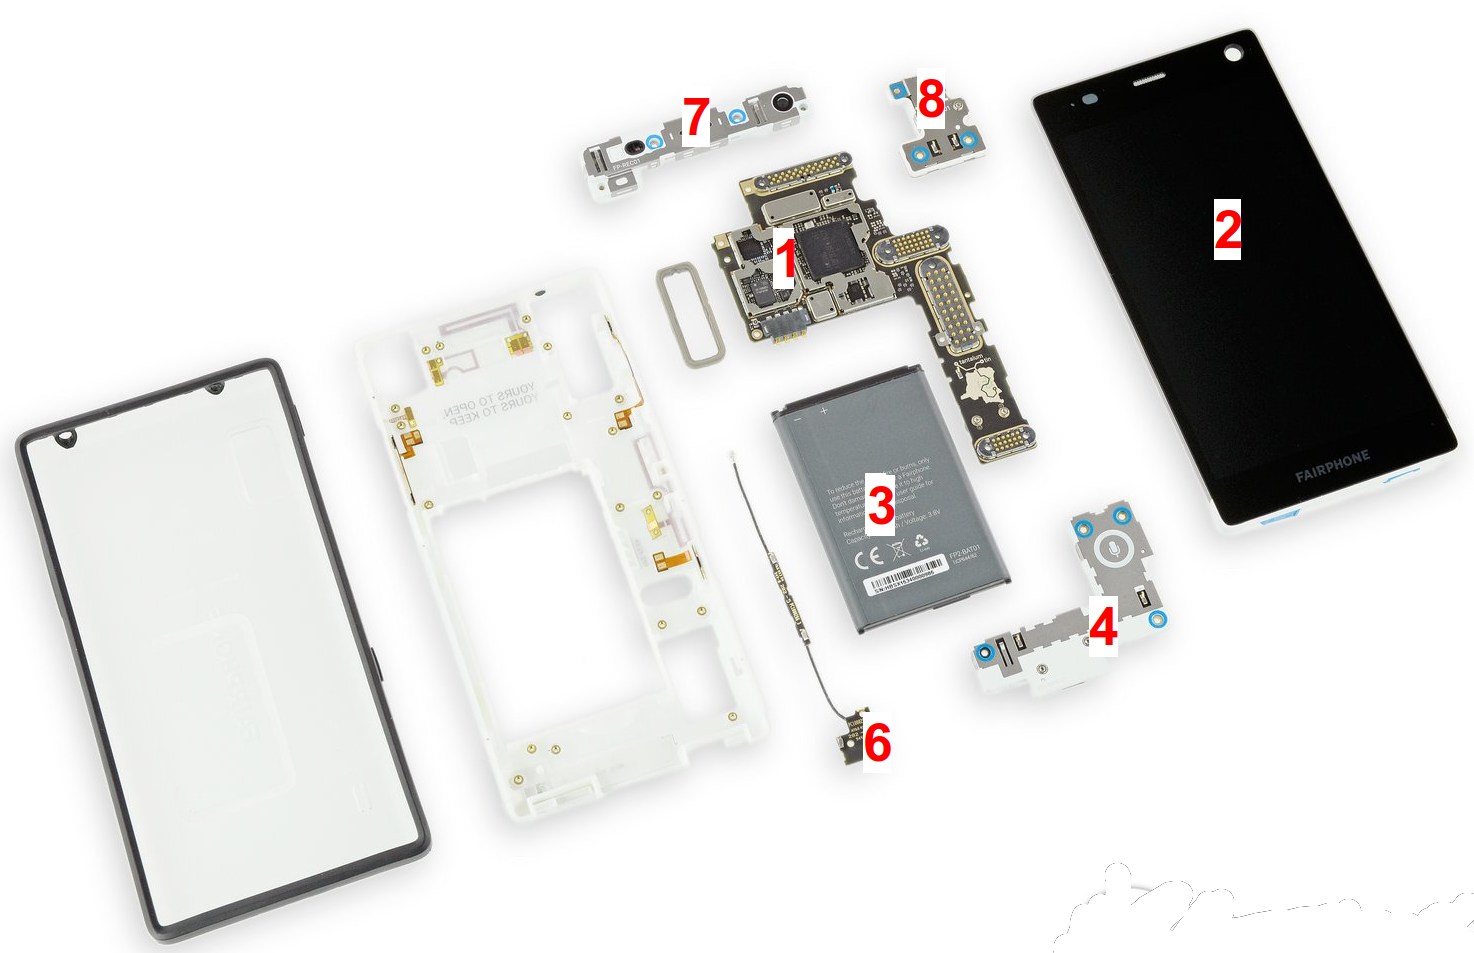
\includegraphics[width=0.9\textwidth]{Images/ordinateur/fairphone}
	\caption{Exemple d'un Fairphone 2. Le téléphone est facilement réparable, chaque composant peut être démonté.}
\end{figure}

Le téléphone est alimenté par une batterie (3). Sur la carte mère (1) on retrouve le processeur (8) qui est superposé à la mémoire (RAM), ainsi qu'une mémoire flash (9) qui fait office de mémoire persistante. 
\begin{figure}[h!]
	\centering
	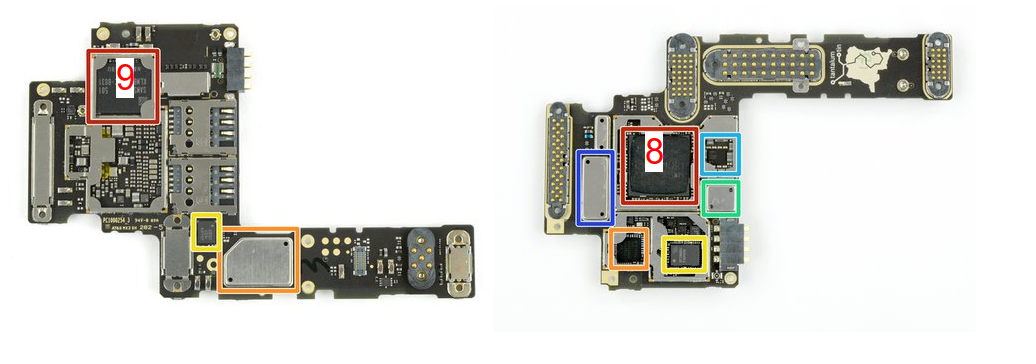
\includegraphics[width=0.9\textwidth]{Images/ordinateur/fairphoneCarteMere.png}
	\caption{Les deux face de la carte mère d'un Fairphone 2.}
\end{figure}

\begin{eclairage}
	Afin de diminuer la dimension des smartphone, c'est souvent le {\bf SoC, (system on a chip)} qui rassemble quasiment tous ces composants: CPU, GPU (processeur de la carte graphique), modem (connexion réseau), mémoire RAM... Dans une petite puce (M1 ou A11 par exemple chez apple ou Exynos chez Samsung) se retrouve concentré la puissance d'un ordinateur d'il y a quelques années.
\end{eclairage}
	

\section{Les serveurs}
Il existe des ordinateurs plus puissants qui sont spécialement conçus pour fournir des informations et des logiciels à d'autres ordinateurs reliés via un réseau. On les appelle des {\bf serveurs}. Ces derniers sont capables de traiter des charges de travail plus importantes et d'exécuter davantage d'applications.

\begin{figure}[h]
	\centering
	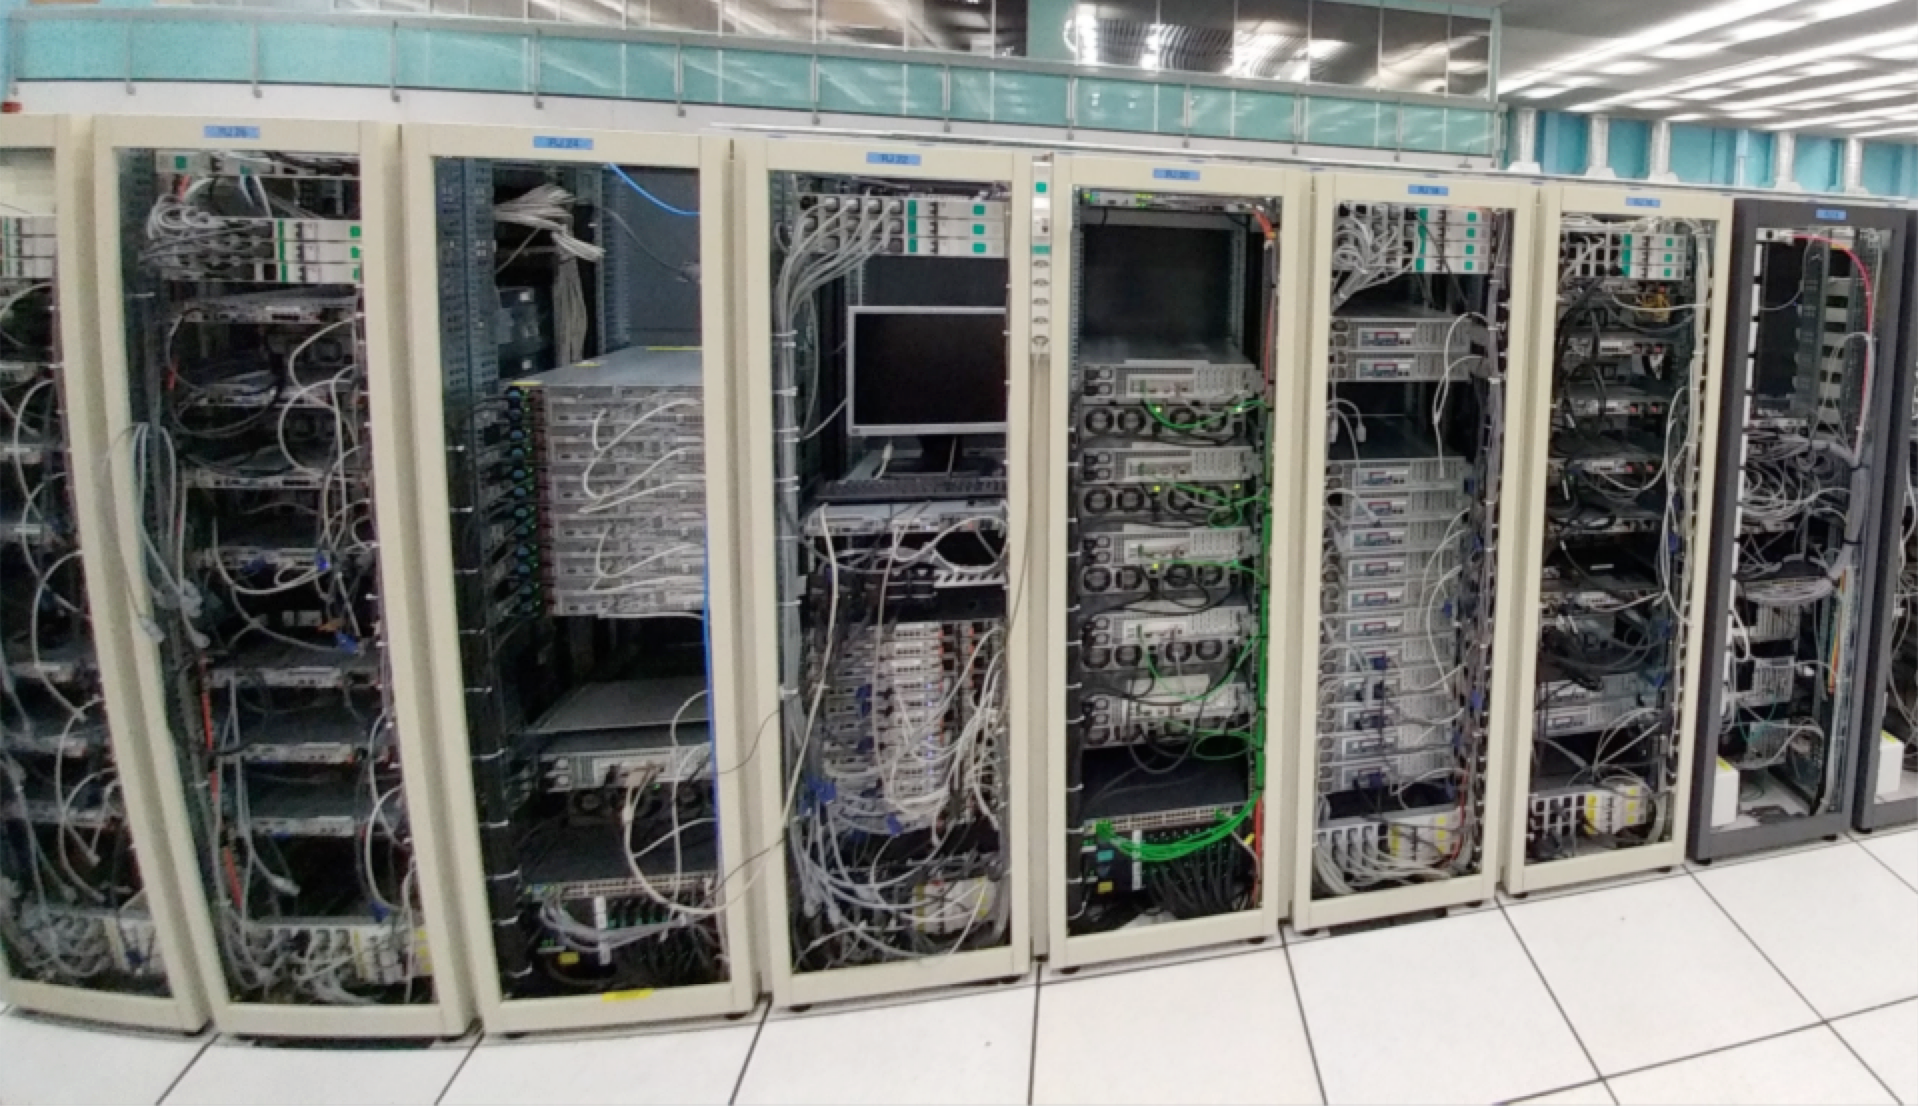
\includegraphics[scale=.4]{Images/ordinateur/serveur}
	\caption{Salle de serveurs du CERN}
	\label{serveur}
\end{figure}


Les ordinateurs les plus puissants au monde sont appelés supercalculateur. Ils contiennent des centaines, voire des milliers de processeurs. Ils sont souvent utilisés dans la recherche médicale, les applications scientifiques (cf Figure \ref{serveur}), le domaine de la finance, la météorologie et à des fins militaires.


\mainsection{\the\numexpr \thechapter + 1 \relax}{Fonctionnement d'un ordinateur}{27/09/1982}

%Théorie :
% Distinguer les types de mesure et leurs principaux ordres de grandeur.
%Comprendre les liens entre utilisateurs, périphériques, applications et systèmes d’exploitation.
%
%Pratique :
%Connaître le nom de plusieurs systèmes d’exploitation et les appareils sur lesquels ils sont installés.

\section{Système d'exploitation}
\begin{wrapfigure}[]{r}{0.3\textwidth}
	\centering
	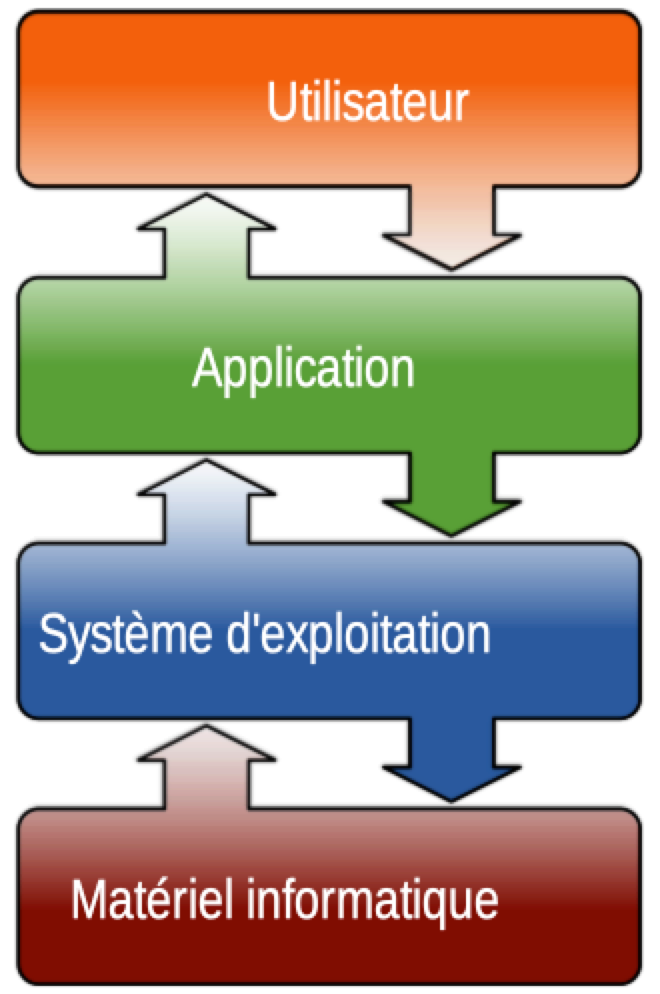
\includegraphics[trim=0 0 0 0,width=0.25\textwidth]{Images/ordinateur/systemeexploitation}
	\caption{Les couches d'abstraction d'un ordinateur.}
\end{wrapfigure}
Vous souhaitez développer un nouveau programme pour smartphone qui va par exemple utiliser la caméra de votre appareil pour prendre des photos. Le problème c'est qu'il existe des centaines de modèles de caméras différent, donc il va vous falloir écrire des centaines de version différentes de votre programme qui chacune sera capable de gérer le bon modèle de caméra (communiquer, s'adapter à la résolution de l'image, etc.). Maintenant vous réalisez qu'il existe aussi des centaines de modèles d'écrans différent, rebelote, il faut de nouveau une centaine de version de votre programme qui devra gérer tous ces écrans et toutes les combinaisons possibles de modèles d'écrans et de caméras!\\

Pour faciliter les choses, on a inventé des programmes bien spécifique qui on pour but de créer un type d'interface (on parle aussi de couche d'abstraction) entre votre application et le matériel de votre ordinateur. Ce programme s'appelle un {\bf système d’exploitation}. Il va permettre à votre application de communiquer avec la caméra de manière générique, peu importe le modèle à partir du moment que la caméra fait des "trucs" de caméra (comme prendre des photos). C'est le système d'exploitation installé sur votre téléphone qui saura comment gérer un modèle spécifique de caméra. Dans ce contexte, il suffit de développer une seule application pour un système d'exploitation précis et l'application fonctionnera sur tous les téléphones qui ont ce système d'exploitation!
\begin{mydefinition}
	Le {\bf système d’exploitation} (noté SE ou OS, abréviation du terme anglais Operating System est un programme qui organise la liaison entre les ressources matérielles (mémoire, accès aux périphériques d'entrées/sorties), l'utilisateur et les applications (traitement de texte, jeu vidéo..). 
\end{mydefinition}	
On pourrait reprendre le même raisonnement que ci-dessus et déduire que pour chaque version d'un système d'exploitation il doit y avoir des centaines de versions différentes car, in fine, un système d'exploitation n'est rien d'autre qu'un programme. En fait, beaucoup de composant sont standardisés, c'est-à-dire qu'ils fonctionnent plus ou moins de la même manière ou avec un nombre restreints de variations. C'est le cas notamment des disques durs, mémoires RAM, souris et clavier. Pour le reste chaque fabriquant fournit un programme appelé \textbf{pilote} (driver en anglais) qui se charge d'expliquer au système d'exploitation comment gérer le composant. 

\begin{mydefinition}
	Un {\bf pilote} (ou {\bf driver} est un programme particulier qui permet la bonne liaison entre le système d'exploitation et le composant (carte graphique, scanner, imprimante...).
	
\end{mydefinition}
\begin{eclairage}
	Le système d'exploitation peut être source d'instabilité (ajouter des bugs) et faire diminuer les performance (programme plus lent, plus de mémoire nécessaire, consommation d'électricité plus importante, ...). De plus, il arrive que notre programme soit destiné à du matériel bien particulier, "l'ordinateur" sera toujours le même. Pour ces raisons, il est parfois souhaitable de se passer de système d'exploitation. C'est notamment le cas, de certains système embarqué, comme le programme qui commande une machine à laver ou un distributeur de billet de banque.
\end{eclairage}
Actuellement, les systèmes d’exploitation les plus connus appartiennent à l’une des deux familles suivantes : la famille unix (Mac OS X et "les Linux"\footnote{On pale ici "des linux" afin de désigner les systèmes d'exploitation basé sur le noyau linux comme Ubuntu, Fedora, Linux Mint,...} pour les ordinateurs, iOS et Android pour les tablettes et smartphones), et la famille Windows. Dans la suite, nous ne décrirons que certains aspects de la première de ces deux familles, étant entendu que les principes généraux que nous allons évoquer sont partagés par tous les
systèmes d’exploitation actuel.

\begin{figure}[h]
	\centering
	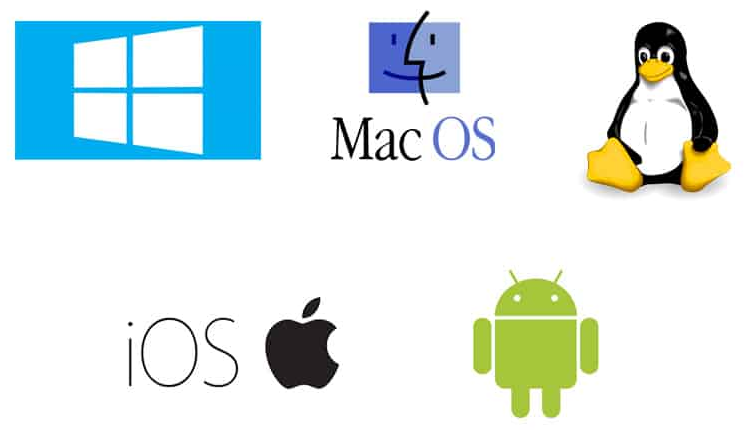
\includegraphics[trim=0 0 0 0,scale=.5]{Images/OS/OS}
	\caption{Différents systèmes d'exploitation}
\end{figure}
Il faut noter que seul le système Linux est \textbf{logiciel libre}.
\begin{eclairage}
	\textbf{Logiciel libre ou logiciel propriétaire ?}\\	
	
	D'après la Free Software Foundation, un logiciel libre (free software) désigne un logiciel qui respecte La liberté des utilisateurs. Ceux-ci ont la Liberté d'exécuter, de copier, de distribuer, d'étudier, de modifier et enfin d'améliorer ce Logiciel. Ainsi, « logiciel libre » fait référence à La « Liberté d'expression ».
\end{eclairage}

\section{L'interface homme-machine}
Le système d’exploitation permet ainsi de « dissocier » les programmes et le matériel, afin notamment de simplifier la gestion des ressources. En outre, il offre  à l’utilisateur une \textbf{interface} homme - machine simplifiée afin de lui permettre de s’affranchir de la complexité de la machine physique. \\


\subsection{*L'interface en ligne de commandes}
Le modèle d'interface le plus basique est le terminal dans lequel l'utilisateur entrer ses commandes par l’intermédiaire de son clavier. L'interface par ligne de commande permet de réaliser des tâches complexes par assemblage d’actions élémentaires. Cet assemblage peut être programmé par un langage de commande (le \textbf{shell} pour les systèmes Unix).\\

Il est aussi possible de développer des programme qui interagirons avec l'utilisateur seulement avec une interface textuelle et qui pourront être exécutés directement dans un terminal. Sous linux, on peut citer
\begin{itemize}
	\item \textbf{top} ou \textbf{htop}: qui permet d'analyser quelles sont les programmes qui sont entrain d'être exécutés sur le système et quelles ressources il utilise (mémoire, CPU, ...).  Ce programme est très utile pour fermer (kill) des programmes qui ne répondent plus ("plantées").
	\item \textbf{nano} : un éditeur de texte basique.
	\item \textbf{convert} : un programme qui permet de convertir des images dans différents formats.
\end{itemize}
\begin{figure}[h!]
	\centering
	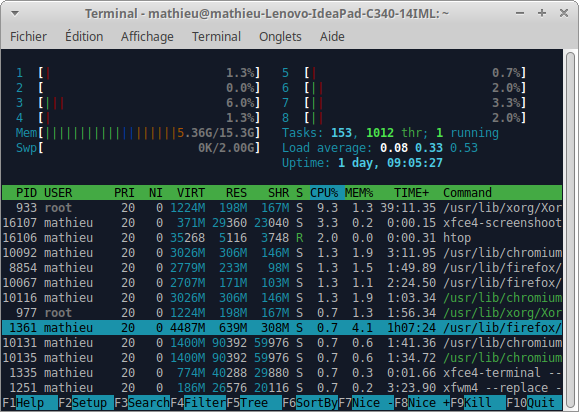
\includegraphics[trim=0 0 0 0,width=0.6\textwidth]{Images/OS/Exemple_terminal.png}
	\caption{Le programme, \textit{htop} lancé dans un terminale Linux}
\end{figure}
\begin{eclairage}
	Sous linux, l’interaction avec le shell se fait généralement par le biais de commandes avec lesquelles les programmes en ligne de commande du même nom peuvent être appelés. Pour chaque action que vous voulez exécuter via le terminal, utilisez un appel de programme selon le schéma de base suivant :
	\begin{lstlisting}[numbers=none]
COMMANDE [OPTIONS] [ARGUMENTS]
	\end{lstlisting}
	Un appel de programme via le terminal est effectué grâce au nom du programme. La plupart du temps, il est possible d’utiliser certaines fonctions supplémentaires grâce à des options. Si un programme attend des arguments (par exemple sous forme de fichiers ou de chemins d’accès à un répertoire), ceux-ci sont généralement spécifiés après les options choisies.\newline \newline
	
	\textbf{Exemple}: J'ai une image, prise avec la caméra de mon téléphone portable, de dimension 3264x2448, stockée dans le fichier "ecole\_sismondi.jpg". Je souhaite redimensionner l'image pour obtenir une image de dimensions 1024 x 768. Ceci peut être obtenu avec le programme \lstinline{convert} avec la commande
	\begin{lstlisting}[numbers=none]
convert  -resize 1024x768 ecole_sismondi.jpg ecole_sismondi_petit.jpg
	\end{lstlisting}	
	Ici les options sont \lstinline{-resize 1024x768}, qui donne la nouvelle résolution, et les arguments \lstinline{ecole_sismondi.jpg}, l'image à convertir, et \lstinline{ecole_sismondi_petit.jpg} le nom de la nouvelle image de dimensions 1024 x 768.
\end{eclairage}	


\subsection{L'interface graphique}
Le développement de l’informatique grand public a conduit à l’apparition d’interfaces graphiques se manipulant à l’aide d’un pointeur dirigé par une souris ou par un doigt (écran ou pavé tactile). Leur avantage est de permettre une utilisation plus intuitive du logiciel d’exploitation.\\

Une interface par ligne de commande reste plus efficace pour un utilisateur aguerri. C’est pourquoi les systèmes d’exploitation modernes continuent de proposer des interprètes de commandes textuelles : c’est le Terminal sous OS X ou Linux et PowerShell sous Windows.

\section{La session utilisateur}
Les systèmes d’exploitation actuels des PCs et des serveurs (et en particulier Unix) sont multi-tâches (plusieurs programmes peuvent être exécutés simultanément) et multi-utilisateurs : ils sont capables de partager des ressources selon une hiérarchie de droits d’accès. Chaque utilisateur se voit attribuer un compte comportant :
\begin{itemize}
	\item un identifiant associé à un mot de passe ;
	\item un répertoire d’accueil personnel destiné à héberger tous les sous-répertoires et fichiers qui lui appartiennent.
\end{itemize}


\section{La mémoire morte vue par l'OS: les fichiers et le système de fichiers}
Le système d'exploitation organise la mémoire morte sous forme de \textbf{fichiers}. Chaque fichier contient des données qui « vont ensemble ». Par exemple, les données d'une image (valeurs des pixels et méta-données) seront stockées dans un même fichier.
\begin{mydefinition}
	Un \textbf{fichier} informatique est un ensemble de données numériques que l'on souhaite faire persister en le stockant sur un support permanent. Un fichier peut être :une image, un film, du texte, un programme source, un programme exécutable, un fichier compressé, etc.
\end{mydefinition}
Comme étudié dans le chapitre sur l'information, les caractères standards (ceux contenus dans la table ASCII) sont toujours codés de la même manière. En revanche, lorsque l'on veut représenter d'autre type de contenus (images, vidéos sons), il existe une multitude de manières possibles. Pour cette raison, on divise les fichiers en trois grandes familles
\begin{itemize}
	\item \textbf{Les fichiers textes}: Chaque octet représente un caractère codé dans la table ascii voir dans une table plus large (pour les caractères spéciaux comme les accents en français). Il fait toujours sens d'ouvrir ce type de fichier avec un éditeur de texte même si les caractère spéciaux peuvent ne pas apparaître correctement;
	\item \textbf{Les fichiers de données binaire}: la représentation de l'information varie en fonction du type d'information ainsi que du codage. il faut un programme spécialisé pour décoder l'information.
	\item \textbf{Les fichiers exécutables}: ce sont les programmes.
\end{itemize}
\subsection{Le nom d'un fichier}
Un fichier comporte un \lstinline{nom_de_fichier}  qui permet de l’identifier et d’y accéder. Ce nom est généralement constitué de deux parties séparées par un point. Par exemple, le fichier nommé  \lstinline{ Recette_tarte_aux_pommes.odt} se décompose :

\begin{center}
	\begin{tikzpicture}
		\filldraw[fill=lightgray] (-1,0.8) rectangle (10,1.6);
		\draw (-1,0) rectangle (10,0.8)
		(-1,0) rectangle (10,1.6)
		(-1,0) rectangle (5,1.6)
		(-1,0) rectangle (7.5,1.6);
		\draw (2.5,1.2) node {\bf Nom du fichier};
		\draw (6.25, 1.2) node {\bf .};
		\draw (8.75,1.2) node {\bf Extension};
		
		\draw (2.,0.4) node {\small  \lstinline{Recette_tarte_aux_pommes}};
		\draw (6.25, 0.4) node {\bf .};
		\draw (8.75,0.4) node {\it odt};
		
	\end{tikzpicture}
\end{center}
Comme le nom du fichier identifie son contenu, il est important de choisir un nom explicite. En effet, si vous nommez votre rédaction de français avec le nom suivant :

$\rightarrow$ \lstinline{ Rédaction_le_petit_prince.odt} : Ce fichier désignera probablement une rédaction avec comme sujet le petit prince.

Par contre, si vous choisissez le nom :

$\rightarrow$ \lstinline{mon_fichier.odt} : Ce nom ne donne aucune information sur son contenu. On n’aura strictement aucune idée de quoi il s’agit sauf qu’il s’agit d’un fichier !

\textbf{Remarques} 
\begin{enumerate}
	\item Pour l’utilisateur, il est donc utile et important de bien choisir un nom qui identifie le contenu de son fichier.
	\item Vous remarquez également que des caractères soulignés ( \_ ) ont été utilisés dans la nomenclature. En effet, pendant longtemps, les espaces n’étaient pas autorisés pour nommer des fichiers, car les espaces étaient utilisés comme séparateurs de nom de fichier ! Actuellement, l’espace est accepté sur la plupart des systèmes, mais il existe toujours de vieux programmes qui refusent un espace dans le nom du fichier ou génère une erreur.
	\item Les caractères accentués (é ê è ü à ä î ô û) étaient également interdits. C’est pour cette raison que l’on trouve souvent des fichiers qui n’ont pas d’accent (merci l’orthographe me direz-vous). À noter qu’il subsiste également d’autres caractères qui sont interdits ou déconseillés:
	\begin{itemize}
		\item Microsoft Windows (interdits) $< \; >  \,  :  \;   " \;   \backslash \;  / \; \vert \; . \; ? \; *$ 
		\item Gnu/Linux et Mac OS (déconseillés): $/$ * 
	\end{itemize}
	\item Les noms ont aussi une limite en longueur, jusqu’à 256 caractères (voir plus pour les tout nouveaux systèmes), mais dans les années 80, le système d’exploitation MS-Dos n’autorisait que 8 caractères plus le point et l’extension de 3 caractères !
	\item Certains systèmes de fichier sont sensibles à la casse, mais pas Microsoft Windows. Exemple avec ces trois noms :
	\begin{enumerate}
		\item {\it recette\_tarte\_aux\_pommes.odt}
		\item {\it Recette\_tarte\_aux\_pommes.odt}
		\item {\it RECETTE\_TARTE\_AUX\_POMMES.odt}
	\end{enumerate}
	Ces trois fichiers indiqueront le même document pour Microsoft Windows, mais bien trois fichiers distincts pour GNU/Linux ou macOS.
\end{enumerate}

\subsection{Format de fichier et extensions}
Lorsque l'on désire lire un fichier qui contient des données, il nous faut connaître
\begin{itemize}
	\item le type d'information qu'il contient (images, sons, vidéos, ...);
	\item la manière dont l'information est codée.
\end{itemize}
Dans ce cas, on parle de \textbf{format de fichier}. Le format du ficher permet de connaître l'encodage utilisé pour stoker l'information. On utilise l'extension du nom du fichier afin d'indiquer quel est le format de fichier utilisé. Les extensions les plus souvent rencontrées sont les suivantes:
\begin{center}
	\begin{tikzpicture}
		\filldraw[fill=lightgray] (-1,8.8) rectangle (12,8);
		\draw (12,-.8) rectangle
		(-1,0) rectangle (12,0.8) rectangle (-1,1.6) 
		rectangle (12,2.4) rectangle (-1,3.2) 
		rectangle (12,4) rectangle (-1,4.8)
		rectangle (12,5.6) rectangle (-1,6.4)
		rectangle (12,7.2) rectangle (-1,8);
		\draw (8,-0.8) -- (8,8.8);
		
		\draw (3.5,8.4) node {\bf Nature du contenu};
		\draw (10,8.4) node {\bf Extensions};
		
		\draw (3.5,7.6) node {\small Document texte libre office writer};
		\draw (10,7.6) node { odt};
		
		\draw (3.5,6.8) node {\small Document tableur libre office calc};
		\draw (10,6.8) node {ods};
		
		\draw (3.5,6) node {\small Document texte Microsoft Word};
		\draw (10,6) node {docx};
		
		\draw (3.5,5.2) node {\small Document tableur Microsoft Excel};
		\draw (10,5.2) node {xlsx};
		
		\draw (3.5,4.4) node {\small Document texte};
		\draw (10,4.4) node {txt};
		
		\draw (3.5,3.6) node {\small Exemples de formats de fichiers compressés};
		\draw (10,3.6) node {zip, rar, tar, gz};
		
		\draw (3.5,2.8) node {\small Exemples de formats de fichiers audio};
		\draw (10,2.8) node {mp3, wav, ogg, flac};
		
		\draw (3.5,2) node {\small Images, photos};
		\draw (10,2) node {png, jpeg, gif};
		
		\draw (3.5,1.2) node {\small Video, film};
		\draw (10,1.2) node {avi, mpg, mov, flv};
		
		\draw (3.5,0.4) node {\small Page web};
		\draw (10,0.4) node {htm, html};
		
		\draw (3.5,-0.4) node {\small Exemples de formats de fichiers de code source};
		\draw (10,-0.4) node {java, c, py};
		
	\end{tikzpicture}
\end{center}

\subsection{L'arborescence}
Usuellement, les fichiers sont regroupés en \textbf{répertoires} ou \textbf{dossiers}. Un répertoire est un conteneur, c'est-à-dire q'il sert simplement à contenir des fichiers ou d'autres répertoires. Les répertoires vont s'imbriquer les uns dans les autres de manière a former une arborescence.

Pour comprendre cette idée d'arborescence, prenons l'exemple de comment un élève pourrait organiser ses documents de cours. Premièrement tous les documents sont stockés dans un armoire, c'est le dossier \textit{\textbf{racine}}. Dans ce dossier racine, il y a un classeur par matière enseigné au collège, chaque classeur correspond à un dossier. Les documents de chacun des classeurs peuvent être regroupés par thème dans des pochettes. Par exemple, dans le classeur géographique, on retrouve une pochette (un dossier) Europe qui contient tous les documents (fichiers) qui traitent de l'Europe.

\begin{figure}[!h]
	\centering
	\subfloat[Analogie]{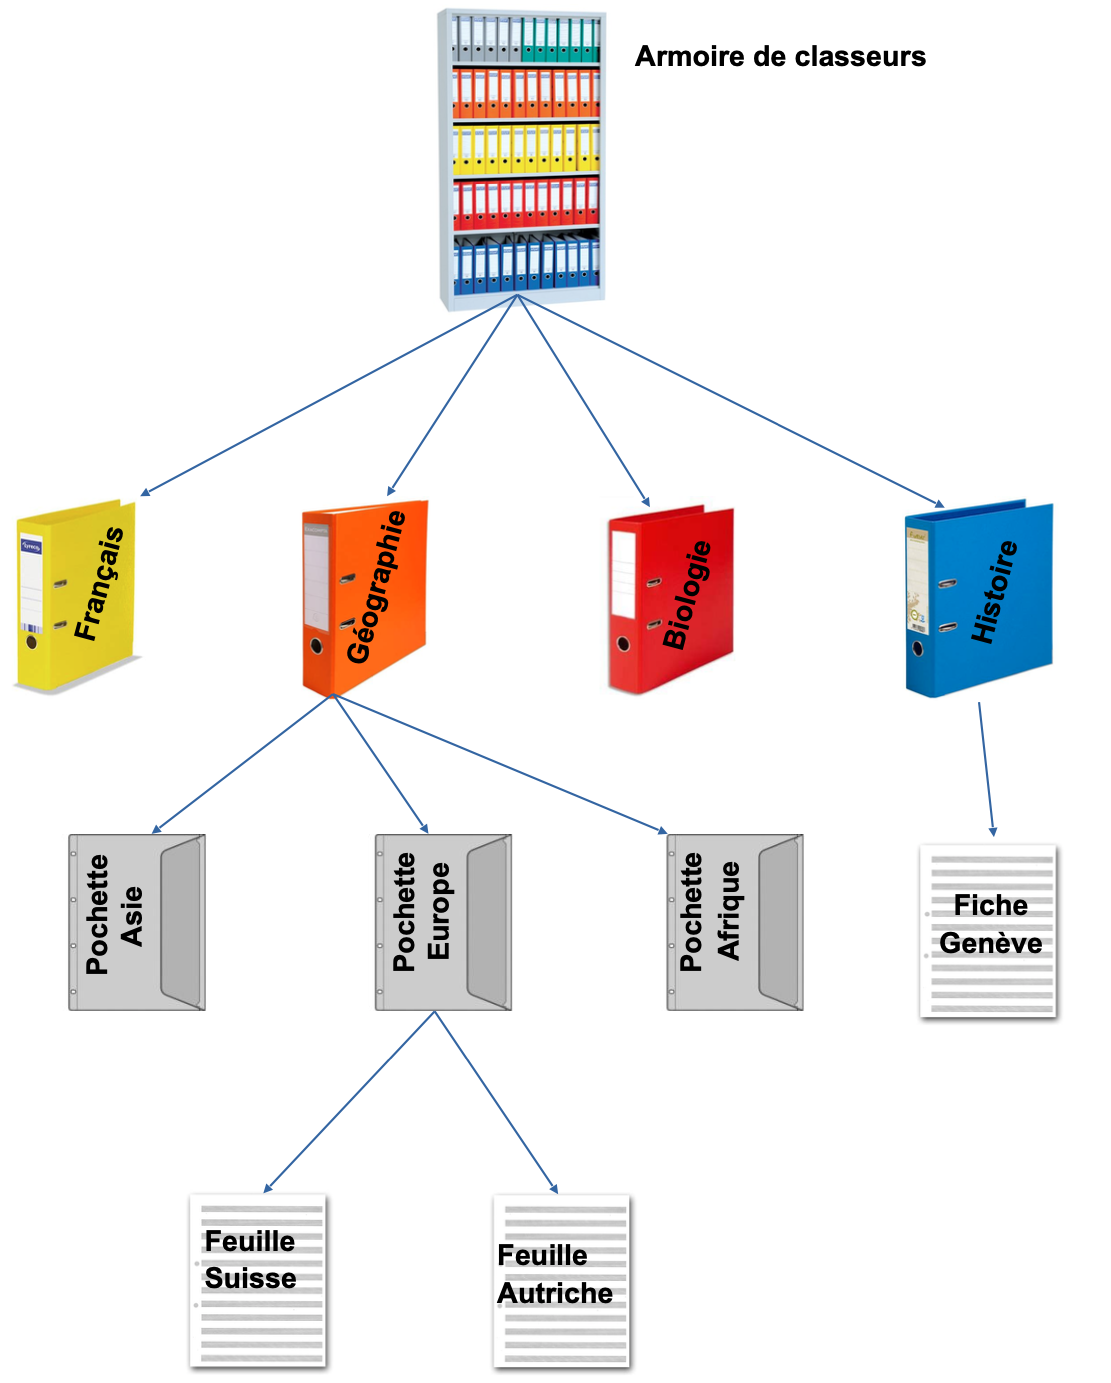
\includegraphics[width=0.4\textwidth]{Images/OS/organisationfichiers}}
	\hspace{1cm}
	\subfloat[Représentation synthétique ]{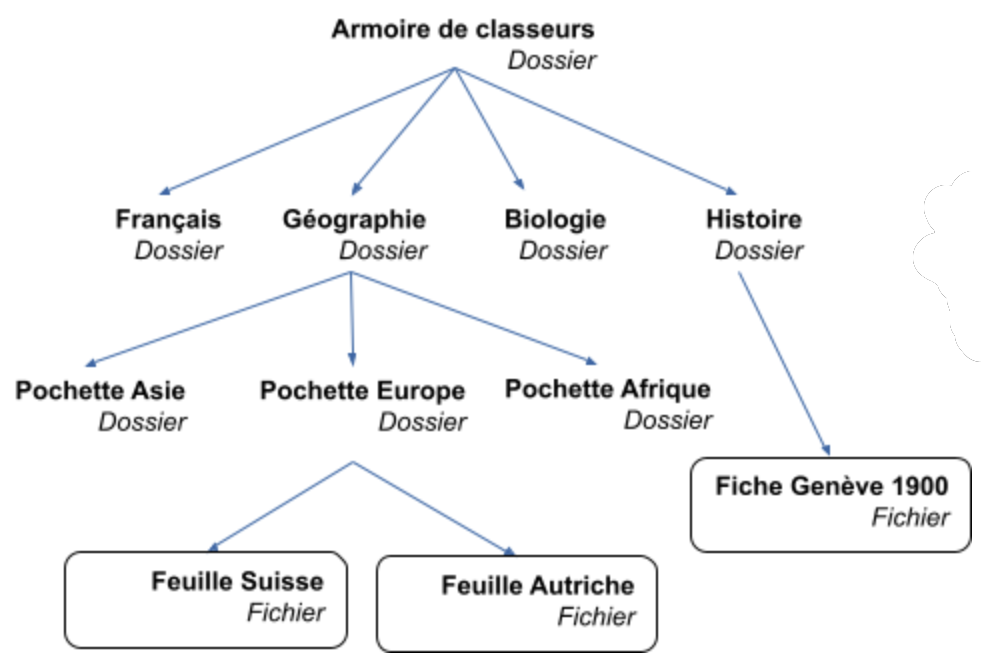
\includegraphics[trim=0 0 100 50, width=0.45\textwidth]{Images/OS/arborescence2}}
	\caption{L'arborescence de fichiers et dossiers.}
\end{figure}\label{CourbeRepr}
Pour résumer: 
\begin{enumerate}
	\item Un {\bf dossier} peut comporter d’autres dossiers et des fichiers.
	\item Un {\bf fichier} est un ensemble organisé d'informations, désigné par un nom précis, que le système d'exploitation d'un ordinateur manipule comme une simple entité, dans sa mémoire persistante.
\end{enumerate}
L’organisation arborescente des fichiers n’est pas le seul moyen de structurer l’information : elle est en concurrence avec d’autres méthodes, parmi lesquelles l’utilisation de liens hypertextes, notion qui n’a pas été inventée pour structurer l’information, mais pour simplifier le mécanisme de référence dans une page web.

\subsection{Le dossier utilisateur}
Les systèmes d'exploitation multi-utilisateurs (ce qui est les cas de Linux, Mac OS X ou Windows) mettent à disposition à chacun de leurs utilisateurs un espace de stockage personnalisé. Cet espace sert principalement à stocker les données propres à l'utilisateur (documents, photos, ...). Un utilisateur peut modifier à sa guise son espace mais ne peut pas, en général, accéder à l'espace d'un autre utilisateur. Il existe cependant la possibilité de \textbf{partager} des dossiers entres plusieurs utilisateurs.

En fonction du système d'exploitation, le chemin d'accès au dossier utilisateur varie. Par exemples, sous
\begin{itemize}
	\item \textbf{Linux}, chaque utilisateur possède un dossier personnalisé dans le répertoire \lstinline{/home};
	\item \textbf{Mac OS X}, chaque utilisateur possède un dossier personnalisé dans le répertoire \lstinline{/Users};
	\item \textbf{Windows 10}, chaque utilisateur possède un dossier personnalisé dans le répertoire \lstinline{C:\Users};
\end{itemize}
\begin{figure}[h!]
	\centering
	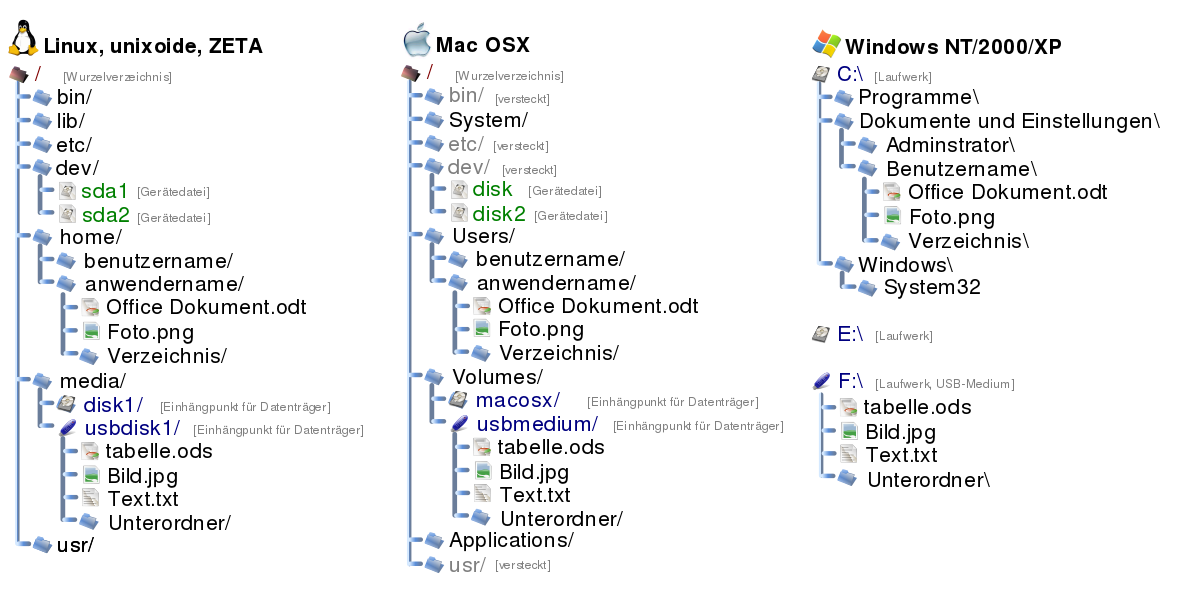
\includegraphics[trim=0 0 0 0,width=0.8\textwidth]{Images/OS/dossier_home.png}
	\caption{Localisation du dossier utilisateur sous Linux, Mac OSX et Windows NT (différent dans les dernières versions de Windows) }
\end{figure}
Dans le dossier utilisateur, on trouve, par défaut, des sous dossiers du type "Mes documents", *mes images", "Téléchargement", "Bureau",...

\subsection{L'arborescence sous Unix (Ubuntu, Android, iOS)}

\begin{mydefinition}
	Un chemin est une liste de répertoire à traverser pour atteindre un fichier ou répertoire donné.
\end{mydefinition}
Tout fichier est référencé par son chemin d’accès, c’est à dire la description du chemin qu’il faut parcourir dans l’arborescence à partir d’un certain répertoire pour atteindre le fichier en question. Le chemin est spécifié par les noms des répertoires séparés par le caractère « / » et suivi du nom du fichier. Lorsqu’on commence la description du chemin par la racine, on dit que le \textbf{chemin est absolu}.
\begin{figure}[h!]
	\centering
	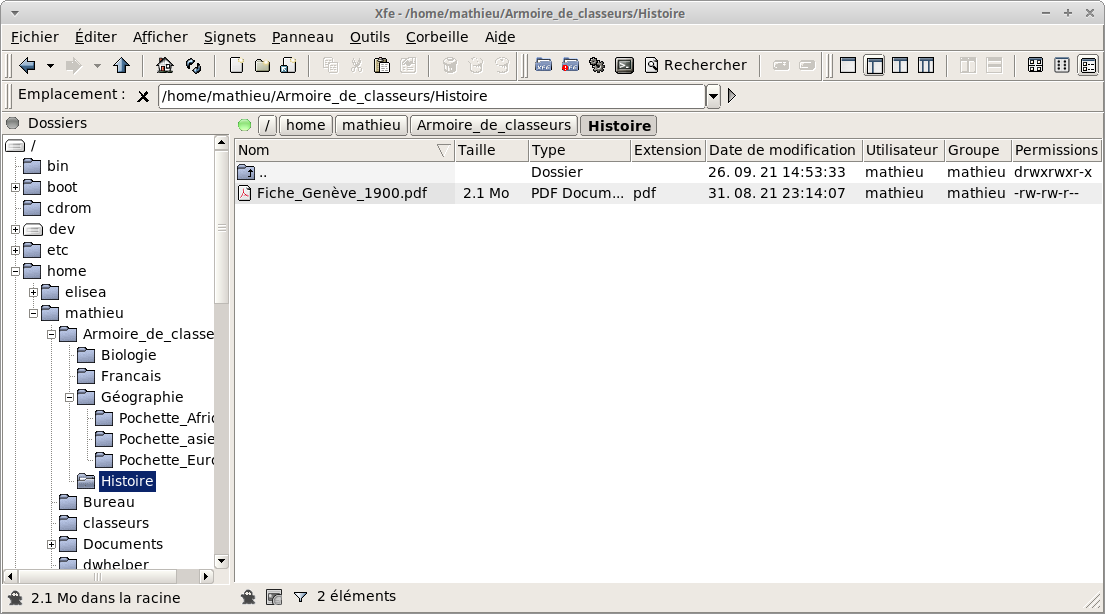
\includegraphics[trim=0 0 0 0,width=0.8\textwidth]{Images/OS/Exemple_arbo_linux}
	\caption{Un arborescence de dossier similaire à l'exemple des classeurs à été crée dans le répertoire du dossier personnel de l'utilisateur "mathieu". Ici, nous visualisons le contenu du répertoire \lstinline{Histoire} qui contient un unique fichier de format PDF et son chemin (absolu) est \lstinline{/home/mathieu/Armoire_de_classeurs/Histoire/Fiche_Genève_1900.pdf}.}
	\label{ex_chemin}
\end{figure}

\begin{important}
	Au collège Sismondi, seuls les enseignant ont un compte utilisateur personnalisé. Tous les élèves se connectent avec le compte  \lstinline{eleve-sismondi}. Dans ce cas, le dossier personnalisé est (en général ?) effacé à chaque nouvelle connexion. Par conséquent, vous devez absolument sauvegarder votre travail, soit sur un clé USB, soit sur un dossier dans le google Drive (\url{eduge.ch}).
\end{important}	
\begin{eclairage}
	 Il est aussi possible de décrire un fichier relativement à la position d’un autre répertoire ; on parle alors de \textbf{chemin relatif}. Dans ce cas, une remontée dans la hiérarchie (accès au dossier parent) est symbolisés par deux points « .. ». Dans l'exemple de la figure \ref{ex_chemin}, le chemin qui part du dossier courant \lstinline{Histoire} vers le dossier \lstinline{Pochette_Europe} est \lstinline{../Géographie/Pochette_Europe}.
\end{eclairage}

Il existe deux moyens pour naviguer dans l'arborescence de fichiers:
\begin{itemize}
	\item Des commandes \lstinline{shell} qui s'utilisent avec une interface en lignes de commandes.
	\item Un explorateur de fichier qui est un programme avec une interface graphique utilisateur.
\end{itemize}

\subsubsection{Navigation avec des lignes de commande*}
Il est possible d’explorer cette arborescente en utilisant un terminal (ou le powershell) et les quelques instructions suivantes
\begin{itemize}
	\item \lstinline{pwd} affiche le répertoire courant ;
	\item \lstinline{ls} affiche le contenu du répertoire courant ;
	\item \lstinline{cd} change le répertoire courant ;
	\item \lstinline{mv} déplace (et renomme) un fichier ou un dossier ;
	\item \lstinline{cp} copie (et renomme) un fichier ;
	\item \lstinline{rm} supprime un fichier ;
	\item \lstinline{mkdir} crée un nouveau répertoire (vide) ;
	\item \lstinline{rmdir} supprime un répertoire vide.
\end{itemize}

 Initialement, le répertoire courant est le dossier personnel de l'utilisateur. Vous pouvez vérifier cette information avec la commande \lstinline{pwd}.
\begin{figure}[h!]
	\centering
	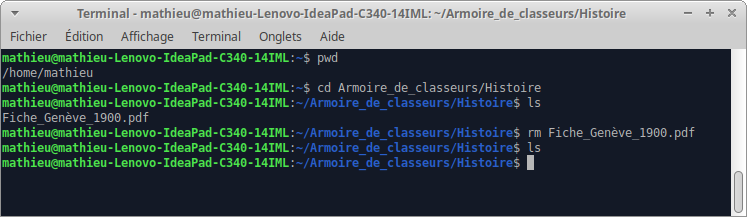
\includegraphics[trim=0 0 0 0,width=0.8\textwidth]{Images/OS/navigation_terminal}
	\caption{L'explorateur de fichiers à partir de lignes de commandes.}
\end{figure}
\begin{important}
	Lorsque l'on supprime un fichier ou un dossier avec les commandes \lstinline{rm} et \lstinline{rmdir}, il sera définitivement supprimé! Il n'ira pas dans la corbeille.
\end{important}	

\subsubsection{Explorateur de fichier}
L'explorateur de fichier permet de naviguer dans les répertoires au moyen de la souris. En général, on trouve un panneau sur la gauche avec un accès rapide au dossier les plus utilisés. Le contenu d'un dossier s'affiche lorsque l'on clique dessus. 
\begin{figure}[h!]
	\centering
	\includegraphics[trim=0 0 0 0,width=0.6\textwidth]{Images/OS/dolphin}
	\caption{Accès aux répertoires fichier depuis un terminal.}
\end{figure}

\mainsection{\the\numexpr \thechapter + 1 \relax}{Stockage de données}{04/10/2021}

%Théorie :
%Être capable de distinguer un support local d’un support distant.
%Pratique :
%Savoir organiser une arborescence. Comprendre la différence entre un fichier et un dossier. Savoir nommer correctement des fichiers et des dossiers. Distinguer différents types de fichiers. 
%Savoir protéger ses données en mettant en place différents types de sauvegarde. Savoir compresser des données. Utiliser un service de stockage distant. Savoir partager des données. Savoir synchroniser des données par le biais d’outils ou de logiciels appropriés.
%Sensibilisation:
%Sensibiliser à l’évolution et à l’obsolescence des supports et des standards. Savoir que le format de stockage dépend du support et du système d’exploitation.


\vspace{-1cm}
\section{Introduction}
\vspace{-0.5cm}
Les besoins en stockage de données numériques, à l’échelle mondiale, ont été multiplié par plus de vingt au cours de la dernière décennie et devraient dépasser les 50 zettaoctets (1 zettaoctet = $10^{21}$ octets) d’ici fin 2021. A titre de comparaison, toute l'information sous format papier sur terre pourrait être stockée en utilisant environ 0,1 zettaoctet. De même, la capacité mémoire totale des tous les cerveaux humains sur la terre serait d'environ 0,001 zettaoctet (\textit{source: Calcul, mémoire, intelligence ?, Jean-Paul Delahaye}).

Comme le montre l’infographie ci-dessous, cette quantité de données produite aujourd'hui apparaît finalement dérisoire en comparaison avec ce qui est attendu pour les quinze prochaines années. Les prévisions tablent en effet sur une multiplication par trois ou quatre du volume annuel de données créées tous les cinq ans. Avec ce rythme exponentiel de croissance, le seuil astronomique des 2’000 zettaoctets devrait être franchi à l’horizon 2035.
\begin{figure}[h!]
	\centering
	\includegraphics[trim=0 0 0 0,width=0.7\textwidth]{Images/stockage/statista.jpeg}
	\caption{Volume annuel de données numériques créées à l’échelle mondiale depuis 2010, en zettaoctets* (\textit{source: Statista Digital Economy Compass 2019}).}
\end{figure}
Il faudrait se procurer 500 millions de disques durs actuels (100 To) pour être capable de sauvegarder 50 [Zo] ! Cette quantité de données pose autant de problèmes de préservation et d’intégrité des données que de sauvegarde. Sans annoncer les problèmes de places, de consommation électrique, de pollutions dues à la fabrication et au recyclage du matériel vieillissant, de coût et de sauvegarde.


\section{Octet (ou byte) : unités de mesure de la quantité de données}
\begin{myrappel}
	L'{\bf octet} (en anglais {\bf byte}) est une unité d'information composée de 8 bits. Il permet, notamment de stocker un caractère comme une lettre ou un chiffre en utilisant le codage ASCII. Un octet permet de représenter $2^8$, c'est-à-dire 256, valeurs possibles.
\end{myrappel}
Jusqu'en 1998; 1024 octets valaient 1 kilooctet. Et depuis les nouvelles unités standardisées par l'organisme international IEC sont les suivantes :
\begin{center}
	\begin{tabular}{| r || c |  c | c | c | c | c | c |  c |}
		\hline
		Symbole & ko & Mo & Go & To & Po & Eo & Zo & Yo \\ \hline
		Nom & kilooctet & mégaoctet & gigaoctet & téraoctet & pétaoctet & exaoctet & zettaoctet & yottaoctet   \\ \hline
		Valeur & $10^{3}$ & $10^{6}$ & $10^{9}$ & $10^{12}$ & $10^{15}$ & $10^{18}$ & $10^{21}$ & $10^{24}$  \\ \hline
	\end{tabular}
\end{center}

\begin{myremarque}
	Il est encore parfois d'usage d'utiliser les préfixes "kilo", "mega", etc. pour désigner des ordres de grandeur qui sont des multiples de $2^{10}=1024$ en non de $10^3=1000$. Par exemple, un mégaoctet devrait en principe valoir $1000 \cdot 1000$ octets, c'est-à-dire 1'000'000 octets, mais il était d'usage de lui attribuer la valeur de  1024 x 1024 octets, c'est-à-dire 1'048'576 octets... ce qui correspond à une différence de 4.63 \% ! Même si ce mésusage tend à disparaître, cette confusion est encore courante.
\end{myremarque}

\section{Comment estimer la quantité nécessaire d'octets pour stocker de l'information}
La taille d'un fichier va dépendre de 
\begin{itemize}
	\item La quantité d'information\footnote{le mot quantité est à prendre dans son interprétation naïve. Il existe une théorie qui définie de manière rigoureuse le concept de quantité d'information, mais ceci dépasse le cadre du cours}, par exemple:
		\begin{itemize}
			\item Le nombre de caractères pour un fichier texte;
			\item Le nombre de pixels pour une image ou une vidéo;
			\item La longueur d'un enregistrement audio ou vidéo;
			\item etc.
		\end{itemize}
	\item La qualité de l'enregistrement, par exemple:	
		\begin{itemize}
			\item Le nombre de caractères différent que peut contenir notre texte;
			\item Le nombre de couleurs (niveaux de gris) possibles pour une image ou une vidéo;
			\item Le nombre d'images par seconde pour une vidéo;
			\item La fréquence d'échantillonnage ainsi que les niveaux d'encodage du signal pour un enregistrement audio
			\item etc.
		\end{itemize}
	\item Si l'information est compressible, par exemple:
		\begin{itemize}
			\item Si il y a de la redondance dans un texte, peu de caractères sont utilisés ou certains caractères apparaissent très souvent comme le "e" en français;
			\item Si il y a des grandes zones uniformes dans une image;
			\item Si on peut supprimer des fréquences d'un enregistrement audio qui ne sont de toute manière pas détectables par la plupart des oreilles humaines.
			\item etc.
		\end{itemize}	
\end{itemize}
On comprend qu'il est difficile d'estimer la taille d'un fichier en se basant sur l'information qu'il contient. On peut cependant donner un ordre de grandeur de taille de fichier en se basant sur les exemples suivants:
\begin{enumerate}
	\item[-] 3 Ko :        fichier texte (3’000 caractère de texte, environ une page A4)
	
	\item[-] 2 à 3 Mo :   image matricielle 1024x768 \textbf{non compressé} avec les couleurs codées sur 24 bits (un octet pour chacune des couleurs de base : \textit{\textbf{R}ed}, \textit{\textbf{G}reen} et \textit{\textbf{B}lue}).
	\item[-] 30 à 100 Ko :    image matricielle 1024x768 \textbf{compressé} avec le format jpeg.
	\item[-] 50 Mo :     fichier audio qualité CD d’une durée ~3 min (débit 320 kbit/s)
	\item[-] 6 Mo :     fichier audio compressé en  MP3 d’une durée ~3 min (débit 320 kbit/s)
	\item[-] 4 Go :     film ~1h30 (qualité DVD)
	\item[-] 20-25 Go :      film ~1h30 (qualité Blu-ray)
	\item[-] 100 Go et plus :     film résolution 4k
\end{enumerate}


\section{Support de données}
Dans ce chapitre, on s'intéresse seulement à la mémoire persistante. Notre distinction sera basée sur l'usage des supports de mémoire plutôt que sur la technologie utilisée.\\

Quel que soit le type de support, sa taille et son emplacement (local ou distant), ils ont tous certains points communs, comme :
\begin{enumerate}
	\item Les supports contiennent des 1 et des 0 qu’il s’agisse de votre dernier livre ou de votre musique préférée.
	\item Tous les supports ont un schéma d’organisation des données qui est dépendante du système d’exploitation.
	\item Ils ont tous besoin d’être alimentés électriquement pour fonctionner.
	\item Aucun support n’est fiable à 100 \% !
\end{enumerate}

\subsection{Mémoire local}
Les disques dur, ou plus récemment, les disques SSD sont les principaux supports de mémoire persistant des PCs. Ils sont rattachés à l'ordinateur et difficilement transportable. En général, dès que le disque est endommagé, toutes les données sont perdues. Il est toutefois possible d'utiliser des technologies amenant de la redondance, par exemple en copiant chaque donnée à double sur deux disques séparés. Cette stratégie est inefficace si la cause du dysfonctionnement d'un disque est externe, par exemple, un incendie.

\subsection{Mémoire transportable : les supports amovibles}
Il est parfois nécessaire de transporter des données. Dans ce cas, on utilise des supports de mémoire amovibles.
Avant d’avoir les clés USB ou les cartes mémoires que l’on retrouve dans les téléphones, il existait d’autres supports externes. Parmi les premiers supports de données informatiques grand public se trouvait la disquette.

\begin{figure}[ht!]
	\centering
	\includegraphics[width=8cm]{Images/stockage/floppy-disk.jpg}
\end{figure}

Inventée dans les années 1970, elle remplaçait les cartes perforées. Quelques exemples de supports amovibles :
\begin{enumerate}
	\item[] 1970 : disquette 8’’ : 1,2 Mo
	\item[] 1970 : disquette 5,25’’ 360k
	\item[] 1980 : disquette 3,5’’: 1,44 Mo, le standard pendant 20 ans !
	\item[] 1990 : CD-ROM 700Mo (d’autre déclinaison jusqu’à 800Mo)
	\item[] 1990 : ZIP : 700Mo
	\item[] 2004 : DVD-ROM : 4,7 Go
	\item[] 2004 : DVD-ROM double couche : 9,4 Go
	\item[] 2006 : Blu-ray 25Go
	\item[] 2006 : Blu-ray double couche 50Go
	\item[] 2000 : clé USB et carte mémoire
\end{enumerate}

\subsection{Supports distants, \textit{solution cloud}}
Avec la multiplication des appareils numérique (PCs, tablettes smartphones, etc.), il est devenu contraignant d'avoirs ses données au même endroit. Par exemple, vous souhaitez accéder à certaines de vos données sur votre tablette à la maison, avec votre téléphone dans le bus ou avec un PC à l'école. 

La rapidité et l'accès à internet à partir de la plupart des ordinateurs ont permis le développement de solutions de stockage accessible à distance. La connexion entre l'ordinateur et un espace de stockage distant, se fait via le réseau internet. On parle de support de mémoire distant ou en nuage (\textit{cloud} en anglais).

\begin{myremarques}
	\item Le terme « cloud » est une forme abrégée de « cloud computing » ou l’informatique en nuage. Un cloud est constitué de serveurs situés à distance et accessibles de n’importe où et à n’importe quel moment via une connexion Internet sécurisée et protégée.
	\item Le terme dématérialisation de l'information est souvent évoquée, mais il ne faut pas s'y tromper, il existe quand même quelque part un support matériel (ou plusieurs) qui stocke vos données. 
\end{myremarques}

\begin{figure}[ht!]
	\centering
	\includegraphics[width=10cm]{Images/stockage/cloud_storage.jpg}
	
\end{figure}

\subsubsection{Avantages et inconvénients d'une solution cloud pour stocker vos données}
\textbf{Exemple d'une offre}\\ L’entreprise \textit{Cloud Prenium} propose un abonnement de 5 chf par mois pour 1 To de place pour vos données. 

\textbf{Question : }Quels sont les avantages et les inconvénients d'une solution en nuage comme celle proposée par \textit{Cloud Prenium}?

\textbf{Avantages principaux du cloud :}
\begin{enumerate}
	\item[+] Vos données sont accessibles partout, à condition d’être connecté à Internet. Vos données sont donc accessibles depuis votre smartphone, votre PC, etc.
	\item[+] Possibilité de partager ses données. De plus, certains logiciels permettent la modification simultanée et gèrent l’accès concurrent.
	\item[+] Aucun investissement ni installation préalable requise, juste le prix de l’abonnement. Il vous suffit en général d’un navigateur web pour accéder à vos données.
	\item[+] Maintenance, sécurisation des données et mises à jour effectuées par le fournisseur.
	\item[+] Souplesse dans l’espace loué. Si vous avez besoin de 2 To, vous pourrez faire évoluer votre abonnement.
	\item[+] En cas de panne de votre ordinateur personnel, vous ne perdez pas les données qui sont dans le cloud.
\end{enumerate}
\textbf{Inconvénients principaux du cloud :}
\begin{enumerate}
	\item[-] Pas de contrôle total d’accès aux données par rapport à l’entreprise \textit{Cloud Prenium}. Confidentialité des données compromise si aucun outil n’est mis en place pour protéger les documents sensibles ;
	\item[-] Savez-vous où sont réellement hébergées vos données ?
	\item[-] Dépendance avec l’entreprise. Si \textit{Cloud Prenium} fait faillite ou son centre de données brule\footnote{\url{https://www.zdnet.fr/actualites/incendie-du-datacenter-de-strasbourg-polemique-autour-des-possibles-negligences-d-ovhcloud-39920937.htm}} que se passe-t-il ? 
	\item[-] Risque de cyberattaques si les données ne sont pas bien protégées.
	\item[-] Obligation d’être connecté à Internet. Le service peut être dégradé si la liaison n’est pas fiable.
	\item[-] Accès aux fichiers plus lents que sur un support local.
	\item[-] Impact écologique : par ses serveurs nécessaires au fonctionnement du cloud, ce dernier induit une consommation d’énergie croissante.
\end{enumerate}
\begin{eclairage}
	En 2016, il était estimé qu'environ 10\% de la production d'électricité du monde était destinée au secteur du numérique. Les \textit{centres de données} accaparaient environ 20\% de ces ressources (source : association negaWatt). 
\end{eclairage}

\section{Stratégie de sauvegarde}
\subsection{Introduction}
Aucun support de stockage n’a une durée de vie illimitée et aucun support de stockage n’est fiable à 100\%. Le risque zéro n’existe pas. Une perte de données numériques est donc très vite arrivée. Les causes principales sont:
\begin{itemize}
	\item des défaillances techniques matérielles comme un disque dur en panne ou une clé usb qui n’est plus accessible;
	\item des défaillances logicielles comme un fichier corrompu suite à une écriture erronée par le système d’exploitation, une erreur de synchronisation;
	\item des défaillances humaines comme un fichier effacé, un fichier écrasé ou une clé usb perdue;
	\item des catastrophes naturelles comme des incendies ou des dégâts des eaux;
	\item des programmes malveillants et des attaques de virus ou de ransomware;
	\item le vol du matériel comme votre téléphone portable, un disque d’un serveur, une clé usb, une carte mémoire;
\end{itemize}
Le monde professionnel indique une durée de vie moyenne de 5 ans pour un disque dur mécanique ou un disque type SSD. Une clé usb ou une carte mémoire de qualité pourrait tenir 10 ans. Le cloud offert par les entreprises de stockage a une durée de vie virtuellement illimitée (voir les inconvénients principaux du cloud).

\subsection{Stratégie 3-2-1 de sauvegarde de données}

La stratégie de sauvegarde 3-2-1 représente le b-a-ba et le minimum de la protection des données. Mise au point par un photographe souhaitant protéger ses clichés dans les années 1920, cette stratégie est devenue une référence, car elle permet une protection optimale des données, quel que soit leur format.

Le concept de base de la stratégie 3-2-1 repose sur trois principes :
\begin{enumerate}
	\item[->] \textbf{{\huge 3} copies de vos données:} La stratégie recommande d’avoir 2 copies plus la source. Avec trois copies dont deux sauvegardes, le risque que les trois copies aient un problème en même temps est très faible surtout si elles sont stockées sur des supports différents.
	
	\item[->] \textbf{{\huge 2} supports différents:} La notion de supports différents est essentielle quand on parle de données numériques, car quel est l’intérêt d’avoir deux sauvegardes si elles sont stockées sur le même support ? En cas d’incident, toutes les données seraient perdues. Il est donc important que la source et au moins une de ses copies soient sauvegardées sur des supports différents.
	
	\item[->] \textbf{{\huge 1} copie hors site:} Quel que soit le support (NAS, disque dur externe, lecteur de bande, etc.), aucune stratégie de sauvegarde de données numériques ne peut être considérée comme sûre si au moins une des copies n’est pas stockée « hors site ». Le récent incendie du 10 mars 2021 d’OVH en est la preuve. En effet, certains utilisateurs avaient leur site en production sur un serveur et leurs copies sur un autre serveur. Certes, les copies étaient sur des supports différents, mais elles étaient stockées dans le même datacenter. Comme une grande partie du site contenant ces serveurs a cessé de fonctionner à cause de l’incendie, aucune des copies n’était utilisable. Or, si au moins une de ces copies avait été stockée chez un autre hébergeur (hors site), ces utilisateurs auraient pu rétablir rapidement leurs services.
\end{enumerate}

Malgré tout les stratégies de sauvegarde ont leurs limites ! La quantité de données à sauvegarder peut prendre trop de temps et poser des problèmes d’intégrité des données. L’externalisation des sauvegardes selon la méthode 3-2-1 soulève aussi la question de la protection des données. 

Et si vous avez bien conservé votre donnée numérique. Serez-vous capable de la relire ?

% reference
% https://pixees.fr/informatiquelycee/prem/index.html

% Thème Algorithmique et programmation
\mainsection{\the\numexpr \thechapter + 1 \relax}{Notions d'algorithmes}{dd/mm/yyyy}

\subsection{Les algorithmes}
Tout d’abord, qu'est-ce qu'un algorithme ? On peut le résumer de la manière suivante :
un algorithme est une méthode générale pour résoudre certains types de problèmes. Il doit
donc, pour chaque instance du problème, se terminer en produisant la bonne sortie, c'est-à-dire résoudre le problème posé.
Gérard Berry résume un algorithme de la manière suivante : un algorithme, c’est tout simplement une façon de décrire dans ses moindres détails comment procéder pour faire quelque chose. 
Donald Ervin Knuth liste 5 propriétés que doit avoir un algorithme :
\begin{enumerate}
    \item \textbf{finitude} : un algorithme doit toujours se terminer après un nombre fini d’étapes;
    \item \textbf{définition précise} : chaque étape d’un algorithme doit être définie précisément les actions à effectuer doivent être spécifiées rigoureusement et sans ambiguïté pour chaque cas;
    \item \textbf{entrées} : un algorithme prend des éléments en entrées qui sont pris dans un ensemble d’objets spécifié;
    \item \textbf{sorties} : un algorithme donne en sorties des éléments ayant une relation spécifiée avec les entrées;
    \item \textbf{rendement} : toutes les opérations que l’algorithme doit accomplir doivent être suffisamment basiques pour pouvoir être en principe réalisées dans une durée finie par un homme utilisant un papier et un crayon.
\end{enumerate}

Les critères de finitude, définition précise et rendrement que Knuth donne, se réfèrent tous au fait qu'un algorithme doit pouvoir être effectivement mis en œuvre, soit par un opérateur, soit par une machine. Aucune ambiguïté d’interprétation des étapes ne doit être possible, chaque étape doit faire référence à une action élémentaire pour l’opérateur et toute exécution de l’algorithme doit se terminer.

La naissance des algorithmes remonte à bien avant le temps des ordinateurs. Les premiers algorithmes ont été découverts chez les Babyloniens en -3000 avant JC. Un algorithme très célèbre est l’algorithme d’Euclide (-300 avant JC) qui permet de déterminer le PGCD de deux nombres entiers positifs. Le premier à avoir systématisé des algorithmes est le mathématicien perse Al-Khwârizmî (entre 813 et 833 après JC). Il a étudié toutes les équations du second degré et en donne la résolution par des algorithmes généraux.

\subsection{Le pseudo-code}
\mainsection{\the\numexpr \thechapter + 1 \relax}{Stratégies algorithmiques}{dd/mm/yyyy}

\mainsection{\the\numexpr \thechapter + 1 \relax}{Introduction à la programmation}{dd/mm/yyyy}

\section{Traitement automatique des données}
Un algorithme permet de résoudre un problème donné au moyen d'un nombre fini d'opérations élémentaires. L'application manuelle d'un algorithme est une tâche fastidieuse. C'est pourquoi l'ordinateur a été inventé dans le but d'automatiser l'implémentation de l'algorithme. On parle de l'informatique comme \textit{la science de traitement automatique de l'information}.\\

Ce  que l'on attend d'un programme c'est qu'il prenne les données d'entrée du problème, qu'il les transforme au moyen de l'algorithme, et qu'il redonne le résultat attendu.
\begin{center}
	\includegraphics[trim=0 0 0 20,width=0.5\textwidth]{Images/shema_science_info}
\end{center}
Pour que le programme s'exécute sur un ordinateur, il faut indiquer à la machine comment si prendre. 
D'un côté l'ordinateur qui comprend seulement le langage binaire composé d'une suite de 0 et de 1 et de l'autre, le programmeur qui parle un langage destiné à la communication entre humains comme le français rempli d'ambiguïtés (plusieurs interprétations possibles de la même phrase). Il faut trouver un intermédiaire, c'est ce qu'on appelle un \textbf{langage de programmation}. 
\begin{mydefinition}
	Un \textbf{langage de programmation} est un langage formel utilisé pour expliquer en détail à un ordinateur comment réaliser une tâche.
\end{mydefinition}
Les langages de programmation sont caractérisés par une \textbf{syntaxe} très rigide (afin qu'aucune ambiguïté n'existe) et qui permet aux ordinateurs d'exécuter ce que les humains leur disent de faire. La syntaxe de codage sera constituée d'ensembles de mots et symboles spécifiques qui devront se combiner  dans un ordre bien particulier (\textbf{règle de syntaxe}). Chaque fois que cet ordre ne sera pas satisfait, l'ordinateur généra une erreur (\textbf{erreur de syntaxe}).
\begin{mydefinition}
	Les \textbf{règles de syntaxe} définissent l’ensemble des programmes qui sont valides et acceptables par l’interpréteur/compilateur.
	En français, les règles de syntaxe incluent l’orthographe et la grammaire, et déterminent quelles sont les phrases valides.
\end{mydefinition}

\begin{eclairage}
	\textbf{Langages naturels Vs Langages de programmation} 
	\begin{multicols}{2}
		\textbf{Langages naturels}
		\begin{itemize}
			\item Communiquer entre humains
			\item Mots corrects (orthographe)
			\item Phrases correctes (grammaire)
		\end{itemize}
		\newpage
		\textbf{Langages de programmation}
		\begin{itemize}
			\item Indiquer à une machine comment résoudre un problème
			\item Identificateurs valides
			\item Syntaxe valide
		\end{itemize}
	\end{multicols}
\end{eclairage}



\section{Langages de programmation}
Pour que le programme écrit dans un langage de programmation soit compréhensible par l'ordinateur il devra être traduit par un programme appelé interpréteur ou compilateur (en fonction du type de langage et de son application). À l'heure actuelle plusieurs centaines de langages de programmation sont utilisés en fonction du domaine, des applications et des préférences du programmeur.
\begin{center}
	\includegraphics[scale=0.45,trim=0 40 0  160,clip=true]{Images/family_tree_languages}
	\captionof{figure}{Arbre généalogique des langages de programmation les plus utilisés.}
\end{center}
Il existe plusieurs critères pour catégoriser tous ces langages de programmation. Nous allons en passer en revue quelques-uns.

\subsection{Paradigmes de programmation}
Selon Wikipedia, \textit{un \textbf{paradigme de programmation} est une façon d'approcher la programmation informatique et de traiter les solutions aux problèmes et leur formulation dans un langage de programmation approprié}. Les paradigmes les plus communs sont 
\begin{enumerate}
	\itemb{programmation impérative}  
	\itemb{programmation fonctionnelle}
	\itemb{programmation orientée objet}
\end{enumerate}
Certains langages de programmation permettent de programmer en utilisant plusieurs approches. C'est notamment le cas du langage Python que nous utiliserons dans ce cours, même si nous adopterons principalement l'approche impérative.

\subsection{Proximité avec le langage binaire-machine}	
On différencie  des langages de programmation  en fonction de leur proximité avec le langage binaire-machine qui est considérée comme le langage de plus bas niveau. On distingue deux niveaux :
\begin{enumerate}
	\itemb{bas niveau (proche machine) :}  permet de contrôler tout ce qui se passe dans la machine pendant l'exécution du code.\\
	C'est un langage machine lisible par un humain qui permet simplement de  manipuler explicitement des registres, des adresses mémoires, voire des instructions machines.  Par exemple~: assembleur, C\ldots.\\
	
	
	\itemb{haut niveau (proche utilisateur) :}  permet à l'utilisateur d'utiliser des fonctions complexes sans se soucier de l'aspect machine (enfin un petit peu quand même).  Pour son optimisation, il utilise parfois (souvent) des langages de bas niveau de façon transparente pour l'utilisateur.  Par exemple : FORTRAN, Python, PHP, SQlite\ldots
\end{enumerate}

\subsection{Langage interprété et langage compilé}		
On peut aussi trier les langages entre langages de programmation interprétés  et langages de programmation compilés:
\begin{enumerate}
	\itemb{interprété :} le langage est lu avec un programme appelé interpréteur pour exécuter le code au fur et à mesure de la lecture du code.  \\
	\begin{tikzpicture} 
		\draw [very thick,->](0,0)node[left]{Code source}--node[above]{\footnotesize interpréteur}++(2.5,0)node[right]{Résultat};
	\end{tikzpicture}
	\begin{enumerate}
		\item{avantage :} Test immédiat 
		\item{inconvénient :} plus lent, le code est interprété à chaque lancement du \textbf{programme interprété}.
	\end{enumerate}
	\itemb{compilé :} le langage est converti en langage machine (binaire) par l'intermédiaire d'un programme dédié (compilateur) qui produit un programme qui pourra dorénavant s'exécuter seul.\\
	\begin{tikzpicture} 
		\draw [very thick,->](0,0)node[left]{Code source}--node[above]{\footnotesize Compilateur}++(2.5,0)node[right](m){code machine};
		\draw [very thick,->](m)--node[above]{\footnotesize exécuteur}++(2.5,0)node[right](m){Résultat};
	\end{tikzpicture}
	\begin{enumerate}
		\item{avantage :} Rapide
		\item{inconvénient :} nécessite une première étape de compilation.
	\end{enumerate}
\end{enumerate}

\subsection{Langages visuels}		
La rigidité et l'austérité des langages de programmation classique a poussé les programmeurs à développer des langages de programmation visuels qui simplifie l'apprentissage de la programmation. Dans un langage visuel, les éléments du langage de programmation sont accessibles sous la forme d’éléments graphiques (le plus souvent des blocs).
\begin{enumerate}
	\item{avantage :} des symboles clairs et une absence  de syntaxe ->  les erreurs de saisie sont impossibles
	\item{inconvénient :} Manque de modularité, il devient très difficile de structurer le programme pour des projets importants.
\end{enumerate}
\begin{figure}[!h]
	\centering
	\subfloat[Langage visuel]{\includegraphics[scale=0.5]{Images/blockly_ex}}
	\hspace{1cm}
	\subfloat[Langage textuel]{\includegraphics[scale=0.5]{Images/micropython_ex}}
	\caption{Le même programme écrit dans deux langages différents.}
\end{figure}\label{CourbeRepr}


\section{La langage \py et l'IDE Thonny}
\subsection{\py}
Quel est le meilleur langage de programmation? Cette seule question a permis de remplir des centaines de forum de programmeurs sur internet. Chaque langage ayant ses avantages, ses particularités et spécificités liées au matériel et type d'applications à créer. Cette année, nous utiliserons le langage \py. Voici un échantillon de raisons qui ont motivé notre choix \footnote{Voir l'article sur  \url{https://linux-center.org/articles/9812/python.html}}:
\begin{itemize}
	\item \py est un langage interprété ce qui rend le code portable sur la plupart des ordinateurs/systèmes d'exploitation.
	\item La syntaxe de \py est très simple. 
	\item Code lisible et compact
	\item \py est gratuit.
	\item \py est très utilisé, en particulier pour l'apprentissage de la programmation.
	\item \py est en 2021 le langage le plus utilisé dans le monde selon la classification\footnote{Voir la classification sur \url{https://spectrum.ieee.org/top-programming-languages-2021}} IEEE\footnote{IEEE: Institute of Electrical and Electronics Engineers ou en français: l'Institut des ingénieurs électriciens et électroniciens} Spectrum 
	\item etc...
\end{itemize}

\subsection{Environnement de Développement Intégré Thonny}
\py est un langage interprété, donc pour écrire des programmes \py nous aurons besoin d':
\begin{itemize}
	\item un éditeur de texte pour écrire le code;
	\item un interpréteur \py pour tester le code ou des instructions;
	\item éventuellement, un débogueur pour pouvoir exécuter les instructions du programme les unes après les autres afin d'identifier les erreurs de programmations.
\end{itemize}
Un logiciel comme \textbf{Thonny}, intègre ces différents aspects dans un seul logiciel, on appelle ce type de logiciel un  Environnement de  Développement Intégré (IDE en anglais pour \textit{Integrated Development Environment}),
\begin{figure}[!h]
	\centering
	\includegraphics[scale=0.5]{Images/IDE_Thonny_illustre-crop.pdf}
	\caption{IDE Thonny}
\end{figure}
\subsubsection{Interpréteur \py}
L'interpréteur \py se présente sous la forme d’une fenêtre avec des \lstinline{>>>} après lesquels on peut entrer des instructions. En pressant la touche \textit{Entrée} du clavier, \py interprète les instructions et affiche le résultat.

\subsubsection{L'éditeur}
Lorsque l'on souhaite taper une suite de commandes, on préfère créer un script (programme) avec l'éditeur. Ainsi on peut sauvegarder son travail dans un fichier texte. Pour exécuter le code tapé dans l'éditeur, il suffit de cliquer sur le bouton vert avec la pointe de flèche.
\begin{important}
	On utilisera l'extension .py pour enregistrer les fichiers qui contiennent du code \py. De plus, on veillera à utiliser un nom de fichier cours mais explicatif sans utiliser d'accent et d'espace (les espaces peuvent être remplacer par le caractère \_ \textit{underscore})
\end{important}


\subsection{Première rencontre avec un programme Python}
Dans un langage impératif, un programme est constitué d'instructions qui vont de la première à la dernière lignes. Comme nous le verrons pas la suite, l'ordre d'exécution entre la première et la dernière instruction pourra varier en fonction d'instructions de contrôle de flux. Prenons le programme, écrit en \py, suivant:

\vspace{-0.7cm}
\begin{monprogramme}
	\lstinputlisting[label={premierprg}, caption=Premier programme Python ]
	{Codes/into_lang_prog/premier_prog_python.py}
\end{monprogramme}
%
\begin{question}
	Que fait ce programme?
\end{question}


\begin{eclairage}
	Le but d'un programme est de traiter de l'information en entrée afin de produire le résultat attendu en sortie. Par conséquent, on retrouvera souvent la structure suivante:
	\begin{itemize}
		\item Une partie entrée où les données du problème sont obtenus (lignes 2 à 5 dans le programme \ref{premierprg}).
		\item Le corps du programme où un algorithme est exécuté instruction après instruction en fonction des données lues (lignes 7 à 13 dans le programme \ref{premierprg});
		\item Une partie sortie qui affiche ou stocke le résultat obtenu (ligne 15 dans le programme \ref{premierprg}).
	\end{itemize}
	Nous verrons par la suite qu'un programme est essentiellement constitué d’expressions ou structures de données et d’instructions ou structures de contrôles. Il contiendra toujours les 4 ingrédients de base suivants
	\begin{itemize}
		\itemb{des structure de données} : les variables (qui représenteront l’Information).
		\itemb{3 types de structures de contrôle du flux d’instructions} (qui permettront de traiter cette Information) :
		\begin{itemize}
			\item Les séquences d’instructions.
			\item Les tests conditionnels ou alternatives.
			\item Les boucles ou répétitions.
		\end{itemize}
	\end{itemize}
\end{eclairage}

\mainsection{\the\numexpr \thechapter + 1 \relax}{Types et opérations}{dd/mm/yyyy}

Tous les langages de programmation ont été crées dans le même but \textbf{traiter de l'information}. Dans un langage impératif, on retrouve toujours les trois concepts suivant 
\begin{itemize}
	\itemb{La notion de valeur} qui représente l'information.
	\itemb{La notion d'expression} qui produit une valeur
	\itemb{La notion d'instructions ou de structure de contrôle} qui utilise des valeurs pour exécuter des commandes d'une manière bien spécifique.
\end{itemize}

\subsection{La notion de valeur}
Une valeur est une représentation de l'information. Par exemple le nombre entier \lstinline{3} représente une valeur, de même que la chaîne de caractères \lstinline{"Hello world"} ou le tableau de nombres à virgule flottante \lstinline{[7.31, 1.74, 3.14, 10.0]}  (similaire aux nombres décimaux). Une valeur est toujours associée à un type (nombre entier/virgule flottante, chaîne de caractères).\\

\subsection{La notion d'expression}
Des valeurs, des opérateurs mathématiques et des parenthèses peuvent former une expression. Une expression est évaluée et le résultat de cette évaluation donne une valeur. 
\begin{mydefinition}
	Une expression est le résultat d'un calcul effectué par le programme. Elle fournit une valeur associé à un type.
\end{mydefinition}

On peut utiliser l'interpréteur python pour évaluer des expressions
\begin{myexample}
	\begin{lstlisting}[numbers=none]
>>>(1 + 2) * (3 + 4)
21
	\end{lstlisting}
	Ici l'expression produit la valeur \lstinline{21} qui est de type entier.
\end{myexample}

\subsection{La notion d'instructions ou de structure de contrôle}
Les \textbf{structures de contrôle} permettent de gérer le flux d'exécution d'un programme, c'est-à-dire l'ordre dans lequel les \textbf{instructions} seront exécutés. Une instruction peut être interprété comme une commande ou un ordre que l'on donne à la machine. En \py, il y deux types d’instruction:
\begin{itemize}
	\item affectation : qui effectue un calcul et qui le stock en mémoire dans une variable.
	\item fonction    : qui est une "commande" prédéfinie. 
\end{itemize}
\begin{myexample}
	\vspace{-3mm}
	\begin{lstlisting}[numbers=none]
>>> x = 1 + 2       # c'est une affectation
>>> print(x)        # c'est un appel à une fonction
3
	\end{lstlisting}
	\vspace{-3mm}
\end{myexample}
%\begin{mdframed}[topline=false,rightline=false,bottomline=false]
%	\hspace*{-\parindent}%
%	\rlap{\smash{\colorbox{white}{\strut\hspace{\parindent}}}}%
%	Les \textbf{structures de contrôle} permettent de gérer le flux d'exécution d'un programme, c'est-à-dire l'ordre dans lequel les \textbf{instructions} seront exécutés. Une instruction peut être interprété comme une commande ou un ordre que l'on donne à la machine. En \py, il y deux types d’instruction:
%\end{mdframed}




\begin{eclairage}
	Tout texte qui suit le caractère dièse "\lstinline{#}" est ignoré par \py, on appelle ceci des commentaires. Leur but est d’expliquer le fonctionnement du programme. C’est une bonne habitude de commenter abondamment le code.
\end{eclairage}
Pour utiliser une instruction, par exemple la \textbf{fonction} \lstinline{print}, il faut lui fournir une valeur (l'information à afficher). Dans l'exemple
\begin{lstlisting}[numbers=none]
>>> print("I love computer science")
I love computer science
\end{lstlisting}\vspace*{-10px}
la valeur à afficher est le message \lstinline{"I love computer science"}. En revanche, la commande 
\begin{lstlisting}[numbers=none]
>>>print(3 * 5 + 2)
17
\end{lstlisting}\vspace*{-10px}
ne produit pas le même résultat que 
\begin{lstlisting}[numbers=none]
>>> print("3 * 5 + 2")
3 * 5 + 2
\end{lstlisting}\vspace*{-10px}
car dans le premier cas la valeur est un nombre qui est le résultat de l'évaluation de l'expression $3\cdot 5 +2$ (un nombre entier), et dans le second la valeur est le message \lstinline{"3 * 5 + 2"} qui est une chaîne de caractère (un message).
\begin{eclairage}
	Les fonctions sont des instructions déjà définies qui font faire quelque chose au programme. La plupart des langages de programmation, par exemple \py, possède toute une série de fonctions prédéfinies qui permettent de réaliser des tâches standard, comme la fonction \lstinline{print} qui permet d'afficher des messages dans l'interpréteur. L'appel d'une fonction s'effectue en indiquant le nom	de la fonction, suivi d'une paire de parenthèses. Ces parenthèses contiennent les éventuels arguments de la fonction, c'est à dire les valeurs nécessaires pour que la fonction puisse être exécutée, séparés par des virgules (exemple \lstinline{print("J'ai ", 16, " ans")}).
\end{eclairage}


\section{La notion de type}
Le type d'information, qu'une valeur peut encoder, varie d'un langage à l'autre. En général, plus le langage est de haut niveau plus il va offrir des types élaborés. La plupart des langages proposent un certain nombre de \textbf{types de base} \footnote{on dit aussi \textbf{types fondamentaux} ou encore \textbf{types primitifs}}. Ils correspondent aux données qui peuvent être traitées directement par le langage. En \py, les quatre types de base incontournables sont
\begin{enumerate}
	\itemb{Les entiers (\lstinline{int}) }:  \lstinline{-4}, \lstinline{0}, \lstinline{99.}\\
	$ \longrightarrow$ Ils servent a représenter des nombres de manières exactes.
	\itemb{Les nombres à virgules flottantes (\lstinline{float})} : \lstinline{20.5 },  \lstinline{10.  } ou \lstinline{ 0.001}.\\
	$ \longrightarrow$ Ils servent a représenter des nombres (éventuellement) approximativement, c’est un genre de notation scientifique en puissance de 2 avec un certains nombres de chiffres significatifs (rappel : en notation scientifique en puissance de $10$, on écrit $7000000001 \approx 7,00 \cdot 10^9$ ).\\
	\textbf{Attention} : On utilise un point pour séparer la partie entière de la partie décimale (ex : 2.68) et non une virgule !
	\itemb{Les chaînes de caractères (\lstinline{str})}: \lstinline{"Hello, World"}, \lstinline{'Oui'.}\\
	$ \longrightarrow$ elles servent a représenter du texte, par exemple lorsque l’on veut afficher une information dans l’interpréteur. Elle sont constituées d'une suite de caractères
	(lettre, chiffre, signe de ponctuation, espace, ...) placées entre guillemets ou (de manière équivalente) entre apostrophes.
	\itemb{Les booléens (\lstinline{bool})}: Seulement deux valeurs possibles \lstinline{True} (vrai) ou \lstinline{False} (faux).\\
	$ \longrightarrow$ Ils servent à représenter \textit{les valeurs de vérité}, par exemple lorsque l'on cherche à évaluer une condition. L'évaluation de l'expression \lstinline{7 < 18} donne la valeur \lstinline{True} tandis que le résultat de \lstinline{0 > 1} donne \lstinline{False}
\end{enumerate}
Les 4 types présentés ci-dessus sont ceux qu'on retrouve dans quasiment tous les langages de programmation. \py, étant un langage de haut niveau, propose une grande quantité de types de bases (voir la liste complète à \url{https://fr.wikiversity.org/wiki/Python/Les_types_de_base}).

\begin{apprendre}
	Pour connaître le type d’une donnée, il suffit de recourir à la fonction \lstinline{type}
	\begin{lstlisting}[numbers=none]
>>> type(10)
<class 'int'>
>>> type(10.0)     #  le type float est caractérisé par un point décimal
<class 'float'>
>>> type("10")     # le type string est caractérisé par les guillemets
<class 'str'>
	\end{lstlisting}
\end{apprendre}


\section{Les opérations}
L’essentiel du travail effectué par un programme consiste à manipuler des données. Peu importe la donnée et son type, ils se ramènent toujours en définitive à une suite finie de bits. Mais alors, pourquoi se compliquer la vie? Deux raisons,
\begin{enumerate}
	\item La taille d'une donnée, c'est-à-dire le nombre de bits nécessaire pour la représenter varie en fonction du type de donné.\\
	Exemple: la chaîne de caractère \lstinline{"c'est trop long"} nécessite plus de bits que le nombre  \lstinline{8}.
	\item Il existe des opérations associé à la plupart des types. Ces opérations vont permettre de transformer l'information en opérant sur les valeurs d'entrées du programme.
\end{enumerate}


\subsection{Opération sur les nombres}
Les opérations sur les nombres sont les suivantes :

\def\arraystretch{1.5}
\begin{table}[h!]
	\small
	\begin{tabular}{llllll|c|l|}
		\cline{7-8}
		&                               &                                   &                                     &                               &                         & \multicolumn{2}{c|}{\footnotesize \textbf{Seulement pour les int}}\\ \hline
		\multicolumn{1}{|l|}{\textbf{opérateur}}                 & \multicolumn{1}{c|}{+}        & \multicolumn{1}{c|}{-}            & \multicolumn{1}{c|}{*}              & \multicolumn{1}{c|}{/}        & \multicolumn{1}{c|}{**} & //                                                                               & \multicolumn{1}{c|}{\%} \\ \hline
		\multicolumn{1}{|l|}{\textbf{signification}}             & \multicolumn{1}{l|}{addition} & \multicolumn{1}{l|}{soustraction} & \multicolumn{1}{l|}{multiplication} & \multicolumn{1}{l|}{division} & exponentiation          & \multicolumn{1}{l|}{\begin{tabular}[c]{@{}l@{}}Division \\ entière\end{tabular}} & Modulo                  \\ \hline
	\end{tabular}
\end{table}
On note que la division entière \lstinline{//} et le modulo \lstinline{%} 
(le reste de la division entière) sont des opérations seulement définies sur les entiers (\lstinline{int}).

\subsubsection{Priorité des opérations}
Comme en mathématique, les opérateurs ont un ordre de priorité. Ainsi si le calcul \lstinline{4+2*3} correspond à \lstinline{4+(2*3)} parce que la multiplication a priorité sur l'addition. L’ordre de priorité est le suivant :
\begin{enumerate}
	\item Exponentiation (Puissance)
	\item Modulo
	\item Multiplication et division entières
	\item Addition et soustraction
\end{enumerate}
Sur les opérateurs de même priorité, c’est celui qui est le plus à gauche qui est évalué en premier. Les parenthèses permettent de changer ces priorités. Leurs effet sera de forcer une opération avant une autre. Par exemple, Si on veut d'abord effectuer \lstinline{4+2} et multiplier le résultat par \lstinline{3}, alors il faut l'indiquer avec des parenthèses : (4+2)*3


\subsection{Opérations sur les booléens et les chaîne de caractère}
Les opération avec les booléens et les chaîne de caractère seront traités dans des chapitres dédiés.


\mainsection{\the\numexpr \thechapter + 1 \relax}{Introduction aux variables}{dd/mm/yyyy}
%voir : http://www.monlyceenumerique.fr/snt_seconde/python/python_en_seconde.html
%voir : https://www.maths-cours.fr/cours/python-au-lycee-1/
%http://info-mounier.fr/snt/python/introduction_variables.php
\vspace{-0.8cm}
\section{Le concept de variable}
\begin{wrapfigure}[]{r}{0.3\textwidth}
	\includegraphics[trim=0 0 0 45,width=0.28\textwidth]{Images/variables/variables}
\end{wrapfigure}
Le but d'un programme est de transformer de l'information. En général, un programme va commencer par stocker en mémoire les données d’entrée qui seront utilisées lors des étapes de traitement. Pour accéder à ces espaces de stockage et savoir quelle genre d'information ils contiennent, il va falloir leur attribuer un nom (ou \textbf{identifiant}) ainsi qu'un \textbf{type}. Pour finir, ces données vont varier au fil de l'exécution du programme, c'est pourquoi on les appelle des \textbf{variables}. Chaque fois qu'on modifie la valeur d'une variable, on dit qu'on lui \textbf{affecte} une nouvelle valeur.
\begin{mydefinitions}
	\item  Une \textbf{variable} est un nom associé à un emplacement de la mémoire. C’est comme une boîte que l’on identifie par une étiquette. On dit aussi que le \textbf{nom de la variable est son identifiant}.
	\item Une \textbf{affectation} est l’attribution d’une valeur (d’un contenu) à une variable
\end{mydefinitions}
Pour résumer, une variable est décrite par
\begin{itemize}
	\item Un \textbf{identifiant} unique qui la désigne.
	\item Un \textbf{type} qui définit de quel « genre » est l’information associée.
	\item Une \textbf{valeur} qui doit respecter le type.
\end{itemize}


\vspace{1cm}
\act Indiquez le type des variables permettant de stocker (sur votre smartphone) les informations suivantes :
\begin{enumerate}[label=\alph*)]
	\item le nom d’un contact
	\item le numéro de téléphone d’un contact
	\item un SMS
	\item l’heure du réveil
	\item le code de votre de votre compte eduge.
	\item le pourcentage affiché de batterie restante
	\item la note de votre dernière évaluation de Mathématiques
\end{enumerate}

\vspace{1cm}

\newpage

\begin{wrapfigure}[]{r}{0.3\textwidth}
	\centering
	\includegraphics[width=0.28\textwidth]{Images/variables/memoire}
	\caption{\small Représentation d'une mémoire d'ordinateur  comme des boîtes. Lorsqu'une variable est crée la boite obtient une \textit{étiquette} (en rouge) et une valeur (en bleu).}
\end{wrapfigure}
Il faut imaginer la mémoire de l’ordinateur comme une grosse armoire avec plein de petites boîtes. 
Certaines de ces boîtes ont un nom (une étiquette) : ce sont des variables, et elles peuvent contenir une valeur. Chaque fois que l'on a besoin de stocker une donnée on va créer une nouvelle variable, en programmation on dira que l'on \textbf{déclare} une variable.

En \py la déclaration d’une variable (et son typage) se fait dynamiquement à l’exécution du programme dès que cette variable apparaît dans une ligne de code. En fait, il suffit d'une \textbf{affectation} en utilisant le symbole "\lstinline{=}". Le code
\begin{lstlisting}[numbers=none]
myInt = 4
myString = "hello"
myReal = 2.5
\end{lstlisting}
crée 3 variables avec comme identifiant \lstinline{myInt}, \lstinline{myString} et \lstinline{myFloat} qui sont de type \lstinline{int}, \lstinline{str} et \lstinline{float} et qui contiennent les données \lstinline{4}, \lstinline{"hello"} et \lstinline{2.5}. 
\begin{center}
	\includegraphics[trim=0 0 0 45,width=0.4\textwidth]{Images/variables/variables2}
\end{center}

\begin{important}
	En \py, les noms de variables doivent en outre obéir à quelques règles simples :\\
	\begin{itemize}
		\item Il est exclusivement composé de lettres (majuscules  et/ou minuscules) et de chiffres mais qui doit toujours	commencer par une lettre.
		\item On ne peut pas utiliser l’un des 33 mots réservés du langage Python
		\begin{multicols}{7}
			\lstinline{and}\\      \lstinline{as}\\         \lstinline{assert}\\      \lstinline{break}\\       \lstinline{class}\\       \lstinline{continue}\\       \lstinline{def}\\
			\lstinline{del}\\       \lstinline{elif}\\       \lstinline{else}\\        \lstinline{except}\\      \lstinline{False}\\       \lstinline{finally}\\        \lstinline{for}\\
			\lstinline{from}\\      \lstinline{global}\\     \lstinline{if}\\          \lstinline{import}\\      \lstinline{in}\\          \lstinline{is}\\             \lstinline{lambda}\\
			\lstinline{None}\\      \lstinline{nonlocal}\\   \lstinline{not}\\         \lstinline{or}\\          \lstinline{pass}\\        \lstinline{raise}\\          \lstinline{return}\\
			\lstinline{True}\\      \lstinline{try}\\        \lstinline{while}\\     \lstinline{with}\\ \lstinline{yield}
		\end{multicols}	
		\item Le Seul symbole autorisé est souligné "$\_$" (underscore en anglais).
		Tous les autres caractères spéciaux sont interdits, en particulier l’espace blanc " " !
		\item Il est sensible à la casse : les minuscules sont différentes des MAJUSCULES. Exemple : les identifiant \lstinline{Age} et \lstinline{age} vont désigner des variables différentes.
	\end{itemize}
\end{important}

\begin{eclairage}
	Il est très important de donner un nom clair et précis aux variables. En lisant le nom de la variable, il faudrait avoir une idée de ce qu'elle représente.
	Par exemple, si je lis \lstinline{note_eleve_JohanS}, je me dis que cette variable représente la note de l'élève Johan S. et donc c'est probablement un \lstinline{float} entre 0.0 et 6.0. Pour améliorer la lecture, on utilise le seul symbole autorisé l'\textit{underscore} "$\_$"\\
\end{eclairage}


\section{L'affectation}
Chaque variable (déclarée) possède une valeur qui est l’information qu’elle porte. Par exemple, la valeur de la variable \lstinline{nombre_eleves_GR103} pourrait être 23, celle de la variable \lstinline{note} pourrait être 4.5, celle de la variable \lstinline{prenom} pourrait être "Anouk".
En \py, pour définir ou modifier la valeur d’une variable, il suffit de lui affecter une valeur en utilisant le symbole égal "\lstinline{=}". 
\begin{mydefinition}
	L’\textbf{affectation} d’une valeur à une variable est l’instruction basique qui permet d’attribuer une valeur à une variable. Par abus de langage, on dit souvent «affectation de variable» ou «assignation de variable».
\end{mydefinition}
En Python, l'affectation s’effectue avec l’opérateur \lstinline{=}. L'instruction d'affectation est composée d'une variable, suivi du symbole égal  \lstinline{=} et d'une expression à évaluer. Après avoir exécutée une affectation la variable prendra la valeur de l'expression évaluée.
\begin{myexample}
	\vspace*{-10px}
	\begin{lstlisting}[numbers=none]
>>> x = (1 + 2) * (3 + 4)
>>> print(x)
21
	\end{lstlisting}\vspace*{-10px}
\end{myexample}

\begin{important}
	\begin{itemize}
		\item 	Il ne faut pas confonde l'opérateur \lstinline{=} (l'affectation) de  l'opérateur \lstinline{==} qui sert à tester l'égalité de deux valeurs. L'opérateur \lstinline{==} est beaucoup plus proche du concept d'égalité utilisée en mathématiques.
		\item l est important de distinguer les expressions, comme \lstinline{x + 2} , des instructions, comme \lstinline{y = x + 2}; . Une expression se calcule, une instruction s’exécute.
	\end{itemize}
	
\end{important}

\subsection{Différents types d’affectations}

\begin{myexamples}
	\itemb{Affectation d'une quantité}
	\begin{lstlisting}[numbers=none]
note = 37 * 50 + 1
	\end{lstlisting}
	\textbf{Explications :}
	\begin{minipage}[t]{0.83\linewidth}
		La valeur \lstinline{37* 50 + 1} (c'est-à-dire \lstinline{4.7}) est injectée dans la case mémoire nommée \lstinline{note}.
	\end{minipage}	
	
	\itemb{Affectation d’un texte}
	\begin{lstlisting}[numbers=none]
prenom = "Robert"
nom_prenom = "Dupont"+'Robert'
	\end{lstlisting}
	\textbf{Remarque :}
	\begin{minipage}[t]{0.85\linewidth}
		Un Chaîne de caractères peut être écrite soit entre "guillemets", soit entre 'apostrophes' droits.
	\end{minipage}
	
	
	\itemb{Affectations parallèles}
	\begin{lstlisting}[numbers=none]
n, x = 1, 7.3
	\end{lstlisting}
	\textbf{Explications :}
	\begin{minipage}[t]{0.83\linewidth}
		C'est équivalent à effectuer les affectations \lstinline{n = 1} et  \lstinline{x = 7.3} simultanément.
	\end{minipage}	
	
	
	\itemb{Auto-affectation}
	\begin{lstlisting}[numbers=none]
k = k ** 2
t = 3 * t - 2
	\end{lstlisting}
	\textbf{Explications :}
	\begin{minipage}[t]{0.83\linewidth}
		Une expression avec la valeur de la variable est calculée puis réaffectée à la variable elle-même.\\
		Par exemple, si \lstinline{t} contient la valeur $5$ alors après avoir exécute \lstinline{t=3*t-2} \lstinline{t} vaudra  \lstinline{3*5-2} (c'est-à-dire \lstinline{13}). 
	\end{minipage}
	
	
	
	\itemb{Incrémentation ou décrémentation}
	\begin{lstlisting}[numbers=none]
k = k + 1
compteur = compteur - 2
	\end{lstlisting}
	\textbf{Remarque :}
	\begin{minipage}[t]{0.85\linewidth}
		Auto-affectation additionnée ou soustraite d’un certain \textit{pas} (d’un certain nombre) entier.
	\end{minipage}
\end{myexamples}
\mainsection{\the\numexpr \thechapter + 1 \relax}{Première structure de contrôle: les tests}{dd/mm/yyyy}

\vspace{-0.8cm}
\section{Introduction}
Sauf mention explicite, les instructions d’un algorithme s’exécutent les unes après les autres, dans l’ordre où elles ont été écrites. Le « chemin » suivi à travers un algorithme est appelé le \textbf{flux d’instructions}, et les constructions qui le modifient sont appelées des \textbf{instructions de contrôle} de flux. On exécute normalement les instructions de la première à la dernière, sauf lorsqu’on rencontre une instruction de contrôle de flux : de telles instructions vont permettre de suivre différents chemins suivant les circonstances. C’est en particulier le cas de l’\textbf{instruction conditionnelle} qui n’exécute une instruction que sous certaines conditions préalables. 

\section{Un exemple}
Par Avec les concepts vus jusqu'ici, un programme exécuté 100 fois de suite donnera 100 fois les mêmes résultats, ce qui présente assez peu d'intérêt. Pour que l'exécution de notre programme dépende de différents paramètres, on utilise des structures de contrôle nommées \textit{instruction conditionnelle}.

La condition est un élément de base d'algorithmique que l'on utilise au quotidien.
\begin{myexample}
	S'il fait beau, j'irai en montagne. 
\end{myexample}
Ces structures permettent d'exécuter ou de ne pas exécuter certaines instructions en fonction de certaines conditions et de changer ainsi le déroulement du programme.


\begin{tabular}{ c  l  }
	Étapes & Instructions \\ \hline
	1 & Se lever  \\ 
	2 & Regarder la météo  \\
	3.1 & S'il fait beau, aller en montagne  \\
\end{tabular}

Un premier moyen d'exprimer des conditions en programmation est l'instruction \textsf{if}. 

\subsection{L'instruction \textsf{if}}
\begin{mydefinition}
	L'instruction \lstinline{if} doit être suivie d'une expression retournant un booléen (\lstinline{True} ou \lstinline{False}) puis d'un symbole \lstinline{:}.  Cette expression peut être une variable contenant un booléen ou une opération retournant un booléen comme les opérateurs \lstinline{<}, \lstinline{>}, \lstinline{==} ou \lstinline{!=}.
\end{mydefinition}

La structure d’une instruction conditionnelle « \lstinline{if} » est la suivante :


\begin{figure}[h!]
	\centering
	\includegraphics[width=0.7\linewidth]{Images/test/if_structure}
	\caption{Figure tirée du livre \textit{Python au Lycée} de Arnaud Bodin}
\end{figure}


\begin{myexample}
	Un premier moyen d'exprimer des conditions en programmation est l'instruction \textsf{if}. En python, elle s'utilise de la manière suivante : 
	
	\begin{lstlisting}[numbers=none]
if meteo == "beau":
   print("Aujourd'hui, je vais en montagne.")
	\end{lstlisting}
	
	Dans cet exemple, si la variable \lstinline{meteo} a été initialisée à \lstinline{"beau"}, la phrase \lstinline{Aujourd'hui, je vais en montagne.} va s'afficher. Si elle a été initialisée à une autre valeur, par exemple \lstinline{meteo = "moche"}, rien ne s'affichera.
\end{myexample}

%\begin{remarque} Le début et la fin du bloc d'instructions soumis à l'instruction |if| sont définis par l'indentation de chaque ligne (le nombre d'espace avant le début du texte). La condition va s'appliquer à tout le bloc d'instruction suivant qui sera décalé vers la droite par rapport à l'instruction |if|. \end{remarque}

\act
On considère les deux programme suivants:
\begin{multicols}{2}
	\lstset{caption={Programme A}}
	\begin{lstlisting}[numbers=none]
if meteo == "beau":
   print("Aujourd'hui, ")
   print("je vais en montagne.")
	\end{lstlisting}
	
	\lstset{caption={Programme B}}
	\begin{lstlisting}[numbers=none]
if meteo == "beau":
   print("Aujourd'hui, ")
print("je vais en montagne.")
	\end{lstlisting}
\end{multicols}

Remplir le tableau en indiquant ce qu'afficher le programme correspondant en fonction de la valeur de la variable \lstinline{meteo}.

\begin{center}
	\begin{tabular}{p{4cm}|p{6cm}|p{6cm}} 
		& \textbf{Programme A} & \textbf{Programme B}  \\ 
		\hline
		\textbf{Cas 1}\par \lstinline!meteo = "beau"! & \  \par\     \  \par\           &              \\ 
		\hline
		\textbf{Cas 2}\par \lstinline!meteo = "moche"! &    \  \par\   \  \par\            &              \\ 
	\end{tabular}
	\arrayrulecolor{black}
\end{center}
\newpage

\subsection{L'instruction \textsf{else}}
L'instruction \lstinline{if} peut être suivie d'une instruction \lstinline{else} qui est exécutée lorsque le résultat du test est \lstinline{False}. Par exemple, on pourrait préciser la situation précédente :  
\begin{myexample} 
	S'il fait beau, j'irai en montagne. Sinon, j'irai au cinéma. 
\end{myexample}
Notre algorithme deviendrait alors : 
\paragraph{}
\begin{tabular}{ c  l  }
	Étapes & Instructions \\ \hline
	1 & Se lever  \\ 
	2 & Regarder la météo  \\
	3.1 & S'il fait beau, aller en montagne  \\
	3.2 & S'il ne fait pas beau, aller au cinéma  \\
\end{tabular}

\paragraph{}
En python, cela s'écrirait de la manière suivante :

\lstset{caption={Instruction \lstinline{if} - \lstinline{else}}}
\begin{lstlisting}[numbers=none]
if meteo == "beau":
   print("Aujourd'hui, je vais en montagne.")
else:
   print("Aujourd'hui, je vais au cinéma.")
\end{lstlisting}

La structure complète d'une instruction conditionnelle avec un bloc "sinon" est la suivante:
% TODO: \usepackage{graphicx} required
\begin{figure}[h!]
	\centering
	\includegraphics[width=0.7\linewidth]{Images/test/if_else_structure}
	\caption{Figure tirée du livre \textit{Python au Lycée} de Arnaud Bodin}
	\label{fig:ifelsestructure}
\end{figure}

\newpage
\subsection{L'instruction \textsf{elif}}
Dans le cas d'une situation non binaire, on peut introduire des conditions supplémentaires qui sont examinées si les conditions précédentes ne sont pas remplies. On peut par exemple nuancer notre situation ainsi : 

\begin{myexample} 
	S'il fait beau, j'irai en montagne. S'il ne fait pas beau et qu'il pleut, j'irai au cinéma. Sinon, j'irai courir au bord du Rhône. 
\end{myexample}

\begin{myremarque} 
	Ici, le terme \textit{Sinon} signifie "S'il ne fait pas beau et qu'il ne pleut pas". C'est pareil en python, l'instruction conditionnée par \lstinline{else} est exécutée si toutes les conditions précédentes sont fausses.
\end{myremarque}


Notre algorithme devient alors : 

\begin{tabular}{ c  l  }
	Étapes & Instructions \\ \hline
	1 & Se lever  \\ 
	2 & Regarder la météo  \\
	3.1 & S'il fait beau, aller en montagne  \\
	3.2 & S'il ne fait pas beau et qu'il pleut, aller au cinéma  \\
	3.3 & S'il ne fait pas beau et qu'il pleut pas, aller courir au bord du Rhône \\
\end{tabular}


En python, on utilise l'instruction \lstinline{elif} qui est la contraction de "\lstinline{else if}" :

\lstset{caption={Instruction if - else}}
\begin{lstlisting}[numbers=none]
if meteo == "beau":
   print("Aujourd'hui, je vais en montagne.")
elif meteo == "pluie":
   print("Aujourd'hui, je vais au cinéma.")
else:
   print("Aujourd'hui, je vais courir au bord du Rhône.")
\end{lstlisting}

\mainsection{\the\numexpr \thechapter + 1 \relax}{Les booléens}{dd/mm/yyyy}

\vspace{-0.8cm}
\section{Vrai ou faux?}
Comme étudié dans le cas des test, un programme se doit de prendre des décisions. Dans notre vie de tous les jours, nos décision dépendent le plus souvent des questions qui se répondent par \textit{oui} ou par \textit{non}. Par exemple, "est-ce qu'il pleut aujourd'hui" ou "êtes-vous mineur". La plupart des langages de programmation comme Python ne possèdent pas de type oui/non mais plutôt un type vrai/faux (\lstinline{True} / \lstinline{False}) qui joue un rôle similaire. Ce type s'appelle \textbf{booléen}. Dans ce contexte, les décisions du programme dépendent plutôt de la véracité d'une \textit{affirmation}. Par exemple, au lieu de répondre à la question "êtes-vous mineur?", on s'intéressera à savoir si l'affirmation "vous êtes mineur" est vraie. Par exemple, en \py, cela ce traduirait par 
\begin{lstlisting}[numbers=none]
age = int(input("Quel est votre age"))
mineur =  age < 18
\end{lstlisting}

Comme étudié dans le chapitre sur les tests, un programme est souvent confronté à devoir prendre des décisions. 
\begin{mydefinition}
	Une \textbf{booléen} est un type de variable à deux états, généralement noté \textit{vrai} (ou 1) et \textit{faux} (ou 0). \\
	
	En langage \lstinline{python},  le type d’une telle variable est \lstinline{bool}, les deux valeurs possibles sont \lstinline{True} ou \lstinline{False}.
\end{mydefinition}

\section{Opérateur de comparaison}
Le plus souvent, un booléen est obtenu lorsque l'on évalue une expression qui compare des valeurs.  Les opérateurs de comparaison sont les suivants
		\begin{center}
	\begin{tabular}{|c|c|l|}
		\hline
		\rowcolor[HTML]{EFEFEF} 
		Opérateur & Expression  & Signification  \\ \hline
		==&      x == y&          Égal   \\ \hline
		!=&     x  != y&          Non égal   \\ \hline
		>&       x > y &         Plus grand que   \\ \hline
		<&      x < y &          Plus petit que   \\ \hline
		>=&      x >= y&         Plus grand ou égal à   \\ \hline
		<=&      x <= y&         Plus petit ou égal à  \\ \hline
		is&       x is y&        est identique  \\ \hline
	  is not&     x is not y&    n’est pas identique   \\ \hline
		
	\end{tabular}
\end{center}
\begin{important}
	Il ne faut pas confondre la simple égalité "\lstinline{=}" qui représente l'affectation de la double égalité "\lstinline{==}" qui teste si deux valeurs sont égales. Par exemple, le programme
	\begin{lstlisting}[numbers=none]
 n = 2**4
 m = 16
 print(n == m)
	\end{lstlisting}
    affiche \lstinline{True} car $2^4$ est égal à $16$.
\end{important}

\exo Dans l'interpréteur Python, taper les lignes suivantes et compléter celles en pointillés.
\begin{lstlisting}[numbers=none]
>>> x=7 
>>> y=17 
>>> x==y
......................................
>>> x!=y
....................................... 
>>> x>y 
..................................... 
>>> x>=y 
..................................... 
>>> x<y 
..................................... 
>>> x<=y 
................................... 
>>> x is y 
................................... 
>>> x is not y 
..................................
\end{lstlisting}

\exo Evaluer le résultat des expressions suivantes
\begin{lstlisting}[numbers=none]
3 == 1 + 2
1.0 == 1 
"1" == 1
3 != 1 + 2
1.0 != 1
1 < 0
"c" <= "h"
"h" > "B"
1.0 is 1 
1 + 2 is not 3
\end{lstlisting}
\begin{important}
	Si les expressions comparées ne sont pas du « même » type, une \lstinline{TypeError} est générée (sauf pour l’opérateur is).	
\end{important}


\section{Opérations  booléens}
Mon réveil sonne le matin lorsque deux conditions sont satisfaites.

\subsection{Recherche internet}
\mainsection{\the\numexpr \thechapter + 1 \relax}{Les boucles}{dd/mm/yyyy}

\vspace{-0.8cm}

\section{Introduction}
En programmation, on appelle boucle un système d’instructions qui permet de répéter un certain nombre de fois (voire indéfiniment) toute une série d’opérations. En Python, comme dans la plupart des langages de programmation il existe deux type de boucle :
\begin{itemize}
	\item La boucle « Pour » (mot-clé \lstinline{for} en Python) qui répète un bloc d’instructions un certain nombre de fois ; Nous découvririons cette boucle en détail dans un prochain cours.
	\item La boucle « tant que » (mot-clé \lstinline{while} en Python) qui exécute un bloc d’instructions tant qu’une condition est vérifée. Dès que la condition devient fausse, elle passe aux instructions qui suivent le bloc :
\end{itemize}



\section{La boucle \textsf{while}}

\begin{mydefinition} La boucle \lstinline{while} permet de répéter un bloc d'instructions tant qu'une condition n'est pas remplie. En python, elle est introduite par le mot-clé \lstinline{while} suivi d'une condition terminé par le symbole ":" 
\end{mydefinition}

\begin{figure}[h]
	\centering
	\includegraphics[scale=1]{Images/boucles/while-loop}
	\caption{Figure tirée du \textit{livre Python} au Lycée de Arnaud Bodin.}
	% Source :  https://openclassrooms.com/fr/courses/7168871-apprenez-les-bases-du-langage-python/7296286-repetez-des-taches-facilement-a-l-aide-de-boucles
	%TODO : make smtg similar in latex 
\end{figure}

\newpage

\begin{myexamples}
	\itemb{Compte à rebours des nombres entre 10 et 0:}\\
	\begin{multicols}{2}
		Le programme suivant  
		\begin{lstlisting}
			
		\end{lstlisting}
	\end{multicols}	
	\item Calculer les premières puissances de 2
\end{myexamples}




\subsection{La boucle \textsf{for}}

Si la boucle |while| est la plus modulable, il existe une boucle plus souvent utilisée car plus pratique dans certains cas : itérer un nombre précis de fois, ou parcourir un tableau, etc. C'est la boucle |for|.


\begin{mydefinition} En python, la boucle |for| permet de répéter un bloc d'instructions pour chaque élément d'un container (tableau, chaîne de caractères, etc.). Elle est introduite par le mot-clé |for| suivi d'un nom de variable, puis du mot-clé |in| et du container à parcourir, et enfin du symbole ":" 
\end{mydefinition}

\begin{figure}[h]\begin{center}
		\includegraphics[scale=.3]{Images/boucles/for-loop}
		\caption{Schéma fonctionnel d'une boucle for}
		% Source : https://openclassrooms.com/fr/courses/7168871-apprenez-les-bases-du-langage-python/7296286-repetez-des-taches-facilement-a-l-aide-de-boucles
		%TODO : make smtg similar in latex 
\end{center}\end{figure}

\begin{myexample}
	L'exemple suivant permet d'afficher la liste des collèges de Genève. Pour chaque élément de la boucle, le programme va exécuter l'instruction print en attribuant à la variable |college| la valeur suivante du tableau.
\end{myexample}
%
%\lstset{caption={Boucle for - parcours tableau}}
%\begin{lstlisting}
%	collegesGe = [ "Alice Rivaz" ,  "Calvin" ,  "Claparède",  "de Candolle", 
%	"de Saussure",  "Rousseau",  "Sismondi",  "Voltaire", 
%	"André-Chavanne", "Emilie Gourd",  "Madame de Stael"]
%	
%	print("Voici la liste des collèges de Genève :")
%	for college in collegesGe:
%	print("Collège", college)
%\end{lstlisting}

\begin{myremarque}
	Dans les cas où l'on veut exécuter un bloc d'instructions un nombre précis de fois, la fonction |range(begin,end)| permet de générer un tableau de |begin| à |end-1| qui peut ensuite être utilisé avec une boucle |for|. L'exemple~\ref{ex:counter} peut ainsi être écrit : 
	
\end{myremarque}

\lstset{caption={Boucle for - compteur trivial}}
\begin{lstlisting}[numbers=none]
	maxCompteur = 10
	for compteur in range(maxCompteur+1):
	print(compteur)
\end{lstlisting}

%
%
%%TODO introduce break, continue, else ?
%

\mainsection{\the\numexpr \thechapter + 1 \relax}{Les chaînes de caractères}{dd/mm/yyyy}

\vspace{-0.8cm}
\section{Opérations de bases}
\mainsection{\the\numexpr \thechapter + 1 \relax}{Les tableaux}{dd/mm/yyyy}

\vspace{-0.8cm}
\section{Opérations de bases}
\mainsection{\the\numexpr \thechapter + 1 \relax}{Les fonctions}{dd/mm/yyyy}

\vspace{-0.8cm}
\section{Code générique}

\begin{appendix}
%\renewcommand{\thesection}{Chap \arabic{section}:}
%\begin{fontsol}
\chapter{Bibliographie}


\begin{enumerate}[label=\textbf{\arabic*}.]
\item  Bernard Gisin, \emph{Cours O.C. d'informatique de 3ème, (2018-2019)}, Collège Claparède, Genève.\\
\item  Germain Gondor, \emph{Informatique pour tous, (2015-2016)}, Lycée Carnot, Dijon.\\
\item  Micha Hersch, \emph{Introduction à la programmation avec Python 3, (2020)}.\\
\item  Mr Jules, \emph{DEBUTER EN PROGRAMMATION PYTHON, (2020)}.\\

\item  Wladston Ferreira Filho, \emph{Computer Science Distilled, (2019)}, Code Energy.\\
\end{enumerate}



\bigskip
%\begin{center}
%\includegraphics[width= 0.8\textwidth]{regle2}
%\end{center}


\end{appendix}
\clearemptydoublepage %% A placer \`a la fin de chaque chapitre pour le verso en page blanche



coucou

\end{document}
